%%% The main file. It contains definitions of basic parameters and includes all other parts.

%% Settings for single-side (simplex) printing
% Margins: left 40mm, right 25mm, top and bottom 25mm
% (but beware, LaTeX adds 1in implicitly)
\documentclass[12pt,a4paper]{report}
\setlength\textwidth{145mm}
\setlength\textheight{247mm}
\setlength\oddsidemargin{15mm}
\setlength\evensidemargin{15mm}
\setlength\topmargin{0mm}
\setlength\headsep{0mm}
\setlength\headheight{0mm}
% \openright makes the following text appear on a right-hand page
\let\openright=\clearpage

%% Settings for two-sided (duplex) printing
% \documentclass[12pt,a4paper,twoside,openright]{report}
% \setlength\textwidth{145mm}
% \setlength\textheight{247mm}
% \setlength\oddsidemargin{14.2mm}
% \setlength\evensidemargin{0mm}
% \setlength\topmargin{0mm}
% \setlength\headsep{0mm}
% \setlength\headheight{0mm}
% \let\openright=\cleardoublepage

%% Character encoding: usually latin2, cp1250 or utf8:
\usepackage[utf8]{inputenc}

%% Further useful packages (included in most LaTeX distributions)
\usepackage{amsmath}        % extensions for typesetting of math
\usepackage{amsfonts}       % math fonts
\usepackage{amsthm}         % theorems, definitions, etc.
\usepackage{bbding}         % various symbols (squares, asterisks, scissors, ...)
\usepackage{bm}             % boldface symbols (\bm)
\usepackage{graphicx}       % embedding of pictures
\usepackage{fancyvrb}       % improved verbatim environment
\usepackage[numbers]{natbib}     
\bibliographystyle{unsrtnat} % order citations by their appearance
\usepackage[nottoc]{tocbibind} % makes sure that bibliography and the lists
			    % of figures/tables are included in the table
			    % of contents
\usepackage{dcolumn}        % improved alignment of table columns
\usepackage{booktabs}       % improved horizontal lines in tables
\usepackage{paralist}       % improved enumerate and itemize
\usepackage[usenames]{xcolor}  % typesetting in color
\usepackage[sc]{mathpazo} % different font to make it a little bit more fun
\usepackage{tabularx}
\usepackage{caption}
\usepackage{rotating}
\usepackage{array}
\usepackage{tikz}
\usepackage{fancyvrb}

%%% Todo notes 
\reversemarginpar
\setlength{\marginparwidth}{3cm}
\usepackage[colorinlistoftodos, textsize=scriptsize, textwidth=30mm]{todonotes}

\usepackage[english]{babel}
\usepackage{csquotes}

%%% Basic information on the thesis

% Thesis title in English (exactly as in the formal assignment)
\def\ThesisTitle{Data-driven Web Application Generator}

% Author of the thesis
\def\ThesisAuthor{Bc. Tobiáš Potoček}

% Year when the thesis is submitted
\def\YearSubmitted{2016}

% Name of the department or institute, where the work was officially assigned
% (according to the Organizational Structure of MFF UK in English,
% or a full name of a department outside MFF)
\def\Department{Department of Software Engineering}

% Is it a department (katedra), or an institute (ústav)?
\def\DeptType{Department}

% Thesis supervisor: name, surname and titles
\def\Supervisor{RNDr. Jiří Helmich}

% Supervisor's department (again according to Organizational structure of MFF)
\def\SupervisorsDepartment{Department of Software Engineering}

% Study programme and specialization
\def\StudyProgramme{Informatics}
\def\StudyBranch{ITI}
% * <tobiaspotocek@gmail.com> 2016-06-07T14:17:16.541Z:
%
% > ITI
%
% Is this correct?
%
% ^.

% An optional dedication: you can thank whomever you wish (your supervisor,
% consultant, a person who lent the software, etc.)
\def\Dedication{%
Dedication.
}

% Abstract (recommended length around 80-200 words; this is not a copy of your thesis assignment!)
\def\Abstract{This thesis is addressing the issue that we are not able to fully utilize the potential of all the data that the contemporary world around us is constantly producing. The goal of this thesis is to implement a Linked Data driven web application generator that allows lay users to generate web applications from multiple  RDF data sources. The application generator automatically analyzes the data sources to help the user with the generation process. Each generated application can be configured and published. The generator contains a list of different types of applications that can be generated depending on the type of input data. This list can be extended and the generator works as a framework which simplifies the process of adding support for new types of applications and new types of data. The generator is also a platform. It allows users to create accounts to manage their published applications and it also features a catalog of published applications and a repository of publicly available data sources that any user can use to generate a new application. The generator is integrated into LinkedPipes Visualization tool. 
}

% 3 to 5 keywords (recommended), each enclosed in curly braces
\def\Keywords{%
{Linked Data}, {LinkedPipes}, {visualization}, {application}, {generator}, {RDF}
}

%% The hyperref package for clickable links in PDF and also for storing
%% metadata to PDF (including the table of contents).
\usepackage[hyphens]{url}
\usepackage[pdftex,unicode]{hyperref}   % Must follow all other packages
\hypersetup{breaklinks=true}
\hypersetup{pdftitle={\ThesisTitle}}
\hypersetup{pdfauthor={\ThesisAuthor}}
\hypersetup{pdfkeywords=\Keywords}
\hypersetup{urlcolor=blue}

% Definitions of macros (see description inside)
%%% This file contains definitions of various useful macros and environments %%%
%%% Please add more macros here instead of cluttering other files with them. %%%

%%% Minor tweaks of style

% These macros employ a little dirty trick to convince LaTeX to typeset
% chapter headings sanely, without lots of empty space above them.
% Feel free to ignore.
\makeatletter
\def\@makechapterhead#1{
  {\parindent \z@ \raggedright \normalfont
   \Huge\bfseries \thechapter. #1
   \par\nobreak
   \vskip 20\p@
}}
\def\@makeschapterhead#1{
  {\parindent \z@ \raggedright \normalfont
   \Huge\bfseries #1
   \par\nobreak
   \vskip 20\p@
}}
\makeatother

% This macro defines a chapter, which is not numbered, but is included
% in the table of contents.
\def\chapwithtoc#1{
\chapter*{#1}
\addcontentsline{toc}{chapter}{#1}
}

% Draw black "slugs" whenever a line overflows, so that we can spot it easily.
\overfullrule=1mm

%%% Macros for definitions, theorems, claims, examples, ... (requires amsthm package)

\theoremstyle{plain}
\newtheorem{thm}{Theorem}
\newtheorem{lemma}[thm]{Lemma}
\newtheorem{claim}[thm]{Claim}

\theoremstyle{plain}
\newtheorem{defn}{Definition}

\theoremstyle{remark}
\newtheorem*{cor}{Corollary}
\newtheorem*{rem}{Remark}
\newtheorem*{example}{Example}

%%% An environment for proofs

%%% FIXME %%% \newenvironment{proof}{
%%% FIXME %%%   \par\medskip\noindent
%%% FIXME %%%   \textit{Proof}.
%%% FIXME %%% }{
%%% FIXME %%% \newline
%%% FIXME %%% \rightline{$\square$}  % or \SquareCastShadowBottomRight from bbding package
%%% FIXME %%% }

%%% An environment for typesetting of program code and input/output
%%% of programs. (Requires the fancyvrb package -- fancy verbatim.)

%%% By tobice: we override the original verbatim environment as 
%%% the verbatim environment is highlighted with a different color
%%% in Overleaf (doesn't work for code)
\DefineVerbatimEnvironment{verbatim}{Verbatim}{fontsize=\scriptsize, frame=single}

%%% The field of all real and natural numbers
\newcommand{\R}{\mathbb{R}}
\newcommand{\N}{\mathbb{N}}

%%% Useful operators for statistics and probability
\DeclareMathOperator{\pr}{\textsf{P}}
\DeclareMathOperator{\E}{\textsf{E}\,}
\DeclareMathOperator{\var}{\textrm{var}}
\DeclareMathOperator{\sd}{\textrm{sd}}

%%% Transposition of a vector/matrix
\newcommand{\T}[1]{#1^\top}

%%% Various math goodies
\newcommand{\goto}{\rightarrow}
\newcommand{\gotop}{\stackrel{P}{\longrightarrow}}
\newcommand{\maon}[1]{o(n^{#1})}
\newcommand{\abs}[1]{\left|{#1}\right|}
\newcommand{\dint}{\int_0^\tau\!\!\int_0^\tau}
\newcommand{\isqr}[1]{\frac{1}{\sqrt{#1}}}

%%% Various table goodies
\newcommand{\pulrad}[1]{\raisebox{1.5ex}[0pt]{#1}}
\newcommand{\mc}[1]{\multicolumn{1}{c}{#1}}


% Title page and various mandatory informational pages
\begin{document}
%%% Title page of the thesis and other mandatory pages

%%% Title page of the thesis

\pagestyle{empty}
\hypersetup{pageanchor=false}
\begin{center}

\centerline{\mbox{
\includegraphics[width=166mm]{img/logo-en.pdf}}}

\vspace{-8mm}
\vfill

{\bf\Large MASTER THESIS}

\vfill

{\LARGE\ThesisAuthor}

\vspace{15mm}

{\LARGE\bfseries\ThesisTitle}

\vfill

\Department

\vfill

\begin{tabular}{rl}

Supervisor of the master thesis: & \Supervisor \\
\noalign{\vspace{2mm}}
Study programme: & \StudyProgramme \\
\noalign{\vspace{2mm}}
Study branch: & \StudyBranch \\
\end{tabular}

\vfill

% Zde doplňte rok
Prague \YearSubmitted

\end{center}

\newpage

%%% Here should be a bound sheet included -- a signed copy of the "master
%%% thesis assignment". This assignment is NOT a part of the electronic
%%% version of the thesis. DO NOT SCAN.

%%% A page with a solemn declaration to the master thesis

\openright
\hypersetup{pageanchor=true}
\pagestyle{plain}
\pagenumbering{roman}
\vglue 0pt plus 1fill

\noindent
I declare that I carried out this master thesis independently, and only with the cited
sources, literature and other professional sources.

\medskip\noindent
I understand that my work relates to the rights and obligations under the Act No.~121/2000 Sb.,
the Copyright Act, as amended, in particular the fact that the Charles
University in Prague has the right to conclude a license agreement on the use of this
work as a school work pursuant to Section 60 subsection 1 of the Copyright Act.

\vspace{10mm}

\hbox{\hbox to 0.5\hsize{%
In ........ date ............	% FIXME!
\hss}\hbox to 0.5\hsize{%
signature of the author
\hss}}

\vspace{20mm}
\newpage

%%% Mandatory information page of the thesis

\openright

\vbox to 0.5\vsize{
\setlength\parindent{0mm}
\setlength\parskip{5mm}

Title:
\ThesisTitle

Author:
\ThesisAuthor

\DeptType:
\Department

Supervisor:
\Supervisor, \SupervisorsDepartment

Abstract:
\Abstract

Keywords:
\Keywords

\vss}

\newpage

%%% Dedication

\openright

\noindent
\Dedication

\newpage

\openright
\pagestyle{plain}
\pagenumbering{arabic}
\setcounter{page}{1}


%%% A page with automatically generated table of contents of the master thesis

\tableofcontents

%%% Each chapter is kept in a separate file
\chapter*{Introduction}
\addcontentsline{toc}{chapter}{Introduction}

The Internet of today is full of data and the amount is constantly increasing. By data we mean literary anything that can be found online, may it be a huge source of organized information like Wikipedia or a small table created with Microsoft Excel by a local government office. Unfortunately, our ability to use the whole potential of all currently available data is very limited. We want to to explore the data, we want to connect and combine different data sets, we want to look for patterns in the data, we want to make the data available to end users. All of that is possible, yet usually time and resources demanding. 

Let us consider for example the aforementioned "Excel table".  XLSX is a proprietary format that can be officially opened only by a paid proprietary software. This software offers a large yet still limited set of tools. It may very well happen that it will not allow us to do what we want. Given the topic of this thesis, let us say that we want to create from the table a new specialized interactive visualization (or an \textit{application}) and publish it online. To get this done,  we would most likely need a computer specialist or  even a developer. Those people are relatively rare and expensive.

Tools that attempt to solve this particular problem are called application generators. They allow non-developers to do developers' work which in this case means to generate from the data an interactive (possibly online) application. Such generators already exist, for example for the aforementioned XLSX format (or in general for tabular data) but they are usually very limited. One reason for this limitation is that the tabular data carry very little semantic information with them. One row represents an entity and each column contains one entity attribute. The first row might (or might not) contain labels for the attributes. That is all that the tabular data based generator can work with.

One of the positive recent trends is that more and more information is published using the Resource Description Framework \cite{rdf} while utilizing the Linked Data model \cite{ld}. Besides being open and offering a natural way of linking and combining different data sets, this framework is able to express any kind of information by extending the raw data with machine-readable semantic meta-data. In other words, data represented in RDF are, unlike the tabular data, not limited in what semantic information they can carry with them. A Linked Data driven application generator could benefit significantly from this feature. As such a generator could literary \textit{understand} the data, it would allow the user to generate way more versatile applications, tailored for all different kinds of data. 
% * <tobiaspotocek@gmail.com> 2016-06-09T10:02:42.253Z:
%
% >  A Linked Data driven application generator could benefit significantly from this feature
%
% Perhaps incorporate somewhere that there already exist lots of existing Linked Data applications but the goal is to make the creation process of new ones simpler.
%
% ^ <tobiaspotocek@gmail.com> 2016-06-09T10:10:59.089Z:
%
% Eg. There is an application called Justinian. It's hard to imagine that a non-developer user could create such a complex application. But the framework could be of great help.
%
% ^.
š
The main goal of this thesis will be to create such a Linked Data driven application generator. That means, as already suggested, that we will be focusing on allowing the non-developers do developers' work. Obviously, that is possible only to a certain extent. The data represented in RDF can be understood with software, but first someone (the developer) has to teach the software how to understand it. For example, for data containing geospatial information (RDF offers a way how to describe such information), the developer would have to extend the generator with a plugin showing such data on a~map.

\section*{Motivation and contribution}
% * <tobiaspotocek@gmail.com> 2016-06-08T21:14:06.686Z:
%
% > Motivation and contribution}
%
% This part should probably go to the Analysis chapter and the Introduction should be kept more general.
%
% ^.
Let us describe more in depth how our application generator will work and how it will help its users. To make it more organized, we will separate the descriptions by different type of users that should benefit from our generator. For each type of user, we will describe his role, his motivation (or perhaps a use case typical for this user) and eventually the contribution of this generator, i. e., how this generator is going to help him.

\begin{itemize}
\item \textbf{Developer}

\textit{Description:} A software engineer with deep technical knowledge.

\textit{Motivation/Use case:} A developer is given a task at his job to create an interactive online map application that visualizes provided company geospatial data. The developer is smart and wants to avoid doing the same thing again the next time. Therefore, he would prefer to create a universal solution that would allow other non-developer employees to create the applications on their own and do it with any data containing geospatial information. Also, it is very likely that he will be given similar task in the near future, but with a different data type and the developer would like to re-use as much work as possible from the first time.

\textit{Contribution:} Thanks to our application generator, the developer will have to focus only on developing the actual visualizer plugin. The generator will work both as a \textit{framework} and a \textit{platform}, solving many problems up front. As as a \textit{platform}, the generator will handle user agenda, registration of new plugins, application management (creating, updating, deleting, publishing), common application configuration and so on. As a \textit{framework}, the generator will define a standard  interface which will allow seamless integration of new plugins. Plus it will provide many drop-in solutions for typical challenges that the developer might encounter across multiple plugins (e.g. caching, multi-language support, support for fixing missing or incorrect data labels, re-usable user interface components etc.).

\item \textbf{Data Analyst}

\textit{Description:} A data analyst is not necessarily a developer, but he has enough knowledge to work with data on a lower level, typically convert data to RDF format or to augment existing RDF data sets with different meta-data. 

\textit{Motivation/Use case:} Let us say that a data analyst works at the same company as our developer. He has a couple of interesting data sets that he would like to make available for other employees so that they could use them to generate applications with the plugin developed by the developer.

\textit{Contribution:} By implementing the interface defined by the framework, each visualizer plugin describes what the input data should look like. Therefore the data analyst has clear instructions on how to prepare a data set to make it compatible with the visualizer plugin. After preparing such data set, the data analyst will be able to upload it to the generator and make it available for all other users that can use the data set for generating new applications.

\item \textbf{User}

\textit{Description: }This is the non-developer with no technical knowledge. He does possess at least some basic understanding of the data though.

\textit{Motivation/Use case: }A user wants to create a new interactive application from a data set and make it available online. For example, he might want to create a map application from the data set with geospatial information, but would be interested only in certain type of data from a certain area.

\textit{Contribution: }The application generator will let this user leverage the work that has been already done by the developer and the data analyst. He will be able to select a prepared data set (or choose his own), the generator will analyze the content of the data set and based on the results, the generator will offer the user a list of visualization plugins that are compatible with the data set. By choosing one plugin, the user will proceed to a configuration phase where he will be allowed to create the application according to his needs. The configuration possibilities will differ depending on the selected visualizer plugin, but typically the user will be allowed filter the data (select a subset) and to tune the level of interactivity for the audience. For example, he could either create a completely static visualization with pre-filtered data, or he could let the audience decide what they want to see. This will greatly increase the re-usability of data sets and visualizer plugins. A single data source with a single visualization plugin will work as a potential source for many applications, each serving a different purpose. None of these applications will involve any more work from the developer or from the data analyst.

Before publishing the application, the user will be allowed to fill missing information (e.g. missing labels in target language) and provide basic application meta data (name and description). After publishing, the application will be available online from a unique URL.

\item \textbf{Audience}

\textit{Description:} The end-user with no knowledge at all, just some basic computer skills.

\textit{Motivation/Use case:} Audience wants to use the application and wants to understand it.

\textit{Contribution:} The application generator will greatly simplify the process of creating new applications which will just by itself result in an increased number of generated applications. Therefore the audience will benefit just from the bare existence of the generator because without the generator, there would be way less applications and the data potential would be wasted. Plus thanks to the configuration phase, the applications will not be just raw visualizations and they will offer better comfort and user experience for the audience.
\end{itemize}

\section*{Goal of this thesis}

The goal of this thesis will be to create a Linked Data based application generator with all the features listed in the previous section. The application generator will work as a \textit{framework}, easily extendable with new visualization plugins that will allow generating applications from different types of data. It will define a clear interface that the new plugins will have to implement. Also many documented drop-in solutions for typical problems and situations will be available for the developer.

The application generator will also be a \textit{platform}, providing space for developers to register new plugins, space for data analyst to publish new data sets and space for common users to generate, manage and publish their applications.

Besides the generator itself, we will also implement two visualizer plugins to demonstrate the abilities of the \textit{framework} and the \textit{platform}.

\section*{Structure of the text}

In Chapter 1, we briefly describe RDF and Linked Data and provide related information necessary for understanding the rest of the thesis. In Chapter 2, we focus on similar existing tools and compare them to our proposed generator. In Chapter 3, we examine in depth the tool LinkedPipes as we will base our generator on top of it.  In Chapter 4, we look more in detail into the required features and we present steps and decisions necessary for achieving our goals. In this chapter, we also analyze and defend our decision to use LinkedPipes as a base for our generator, plus we describe how it has to be modified to fit our intentions. In Chapter 5, we dive into implementation details. Especially we focus on the framework aspect. We show how a new visualizer plugin can be integrated into the generator and what tools are available for the developer. In Chapter 6, we describe in detail the two visualizer plugins, D3.js Chord Visualizer and Google Maps Visualizer, that we implemented to demonstrate our generator's abilities. Related to the D3.js Chord Visualizer, there is a short theoretical part in this chapter that deals with representing and sampling graph structures (actual graphs as understood in graph theory) using RDF and SPARQL queries. In the final Chapter 7, we describe possible future work.
\chapter{Preliminaries}


\chapter{Related Work}
\label{chap:related-work}

In this chapter, we will present several tools with similar focus as our proposed \emph{application generator}. That will help us to identify the key features that we will need to implement in order to achieve our goals. We aim to create a \emph{Linked Data-driven web application generator}. So we have to begin with defining what kind of tools would fall into the same category. Before we start: Let us not limit ourselves only to Linked Data based tools. Firstly, there is not that many similar Linked Data based tools available so there would not be much to analyze. Secondly, we can get interesting findings even from the other tools, as the inner data format is only one aspect of a generator (and for a non-developer, i. e., our potential user, it is definitely not the most important one). We will now move on to the individual features that a tool should have in order to be classified by us as a \emph{data-driven application generator}.

\section{Application generator definition}
\label{sec:rw:definition}

Firstly, such a tool should be a \emph{generator}. That means that whatever the generator produces, it should not disappear after the generator is closed and it should persist as an independent \emph{instance}. This requirement is rather vague as for example any text processor (e.g. Microsoft Word) would count as a generator in this sense. But it does rule out all kinds of \emph{data viewers}. Secondly, such a tool should generate \emph{applications}. An application, to be called an \emph{application}, should offer (at least potentially) some level of interactivity. For example text documents, images or static visualizations (like non-interactive graphs) are definitely not applications. Lastly, such a tool should be \emph{data-driven}. That means that in a typical scenario, one should start the process with a data set and use this data set to create a new application with the generator.  To give you an example of what we do not consider \emph{data-driven}, we could mention for example the WordPress.com \cite{wordpress} platform. This platform definitely is an \emph{application generator} according to our first two requirements (specifically, it is a \emph{website generator}, or perhaps a \emph{blog generator}). The key difference is that when you create a new application (a \emph{website} or a \emph{blog}), it is empty and then you start adding the data. The process is completely reversed.

We admit that all these definitions are rather vague and it can still be hard to determine whether a certain tool falls into the category of \emph{data-driven application generators} or not. We believe, however, that all these definitions together give the reader a decent idea of what we consider a \emph{data-driven application generator}.

\section{Examined features}
\label{sec:rw:features}

To make the comparison more organized, we define a limited set of features that we will specifically focus on while examining the tools. An overview table showing the support of these features among all selected tools will be presented to the reader. Let us now give a short description of each chosen feature.

\begin{itemize}
\item \emph{Linked Data support}. Our \emph{application generator} is going to be Linked Data based and we consider this aspect one of its biggest assets. Therefore we are naturally interested in the \emph{Linked Data support} of other tools as well.
\item \emph{Extendability}. We want to know whether a particular tool can be programmatically extended to support new types of data and new corresponding types of applications. By a type of data we do not mean a different format (the data might or might not be represented in RDF, that is irrelevant at this moment) but a different \emph{semantic} meaning of the data. For example, if we decide that our generator should be able to recognize geospatial data and visualize them using an application in the form of a map, can we extend the generator in such a way? Also just because a particular tool is released under an Open-Source software license and therefore can be modified, we do not consider it \emph{extendable}. Such a tool has to be intentionally \emph{designed} as \emph{extendable} with clearly defined and documented plugin interface.
\item \emph{Data analysis}. We are interested in whether the generator analyses the input data in any way. Typically, such a generator can enable (or disable)  features of generated applications depending on the characteristics of the input data. Or it can give recommendations to the user about how the data can be visualized. We can say that such a generator \emph{understands} the data to a certain extent. By contrast, a generator that performs no analysis at all, leaves the whole generation process up to the user. Then there is the question whether the application is still \emph{generated} or rather just \emph{built} by the user.
\item \emph{Online sharing}. We want to know whether a generated application can be published online.
\item \emph{Non-developers friendly}. Here we are interested in whether the \emph{application generator} can be operated by a person with no technical knowledge. We are focused specifically on the actual application creation process. An expert might be needed to set up the generator, but this requirement would not break this condition.
\item \emph{Platform}. This feature specifies whether the generator exists in the form of an online \emph{platform} where each user has an account through which he can create, publish and manage his applications.
\item \emph{Configuration}. Here we want to know whether the generator will simply take the input data and generate and publish the application, or whether it will offer the user an extra \emph{configuration} step in between, in which the user will be able to affect the final shape of the application before publishing it. This configuration step should allow more than just changing the application name.
\end{itemize}

\def\checkmark{\tikz\fill[scale=0.4](0,.35) -- (.25,0) -- (1,.7) -- (.25,.15) -- cycle;}
\newcolumntype{C}{>{\centering}X} % Create new column type that centers the cell content
\begin{table}[ht]
  \caption{Features of related tools}
  \vspace{0.5cm}
  \label{tab:related-features}
\begin{tabularx}
  {\textwidth}{ |r|C|C|C|C|C|C|C| }
  \hline
      \begin{sideways}Tool\end{sideways} & 
      \begin{sideways}Linked Data support\end{sideways} &
      \begin{sideways}Extendability\end{sideways} &
      \begin{sideways}Data analysis\end{sideways} &
      \begin{sideways}Online sharing\end{sideways} &
      \begin{sideways}Non-developers friendly\end{sideways} &
      \begin{sideways}Platform\end{sideways} &
      \begin{sideways}Configuration\end{sideways} \tabularnewline \hline
  \hline
% 							&LD			&Extend		&Data analysis	&Sharing	&Non-devel	&Platform	&Config	
  Miga Data Viewer			&			& 			&\checkmark	 	&\checkmark &			&			&\checkmark ~ \tabularnewline \hline
  Citadel on the Move		& 			&\checkmark	&				&\checkmark	&\checkmark	&\checkmark	&\checkmark	~ \tabularnewline \hline
  Tableau       			& 			&			&				&\checkmark	&\checkmark	&\checkmark	&\checkmark	~ \tabularnewline \hline
  Avelca                	& 			&			&				&\checkmark	&\checkmark	&\checkmark	&\checkmark	~ \tabularnewline \hline
  Exhibit             		&\checkmark	&\checkmark	&				&\checkmark	&			&			&\checkmark	~ \tabularnewline \hline
  Payola              		&\checkmark	&\checkmark	&				&\checkmark	&\checkmark	&\checkmark &\checkmark	~ \tabularnewline \hline
  LinkedPipes Visualization &\checkmark	&\checkmark	&\checkmark		&\checkmark	&\checkmark	&			&			~ \tabularnewline \hline

\end{tabularx}
\end{table}

\section{Miga Data Viewer}
\label{sec:related-work:miga-data-viewer}

Miga Data Viewer is a tabular data based \emph{application generator}. It accepts only data in the CSV format but as this format is widely supported and there is lots of conversion tools available, any source of tabular data (Microsoft Excel file, RDBMS) can be used as an input. Despite the word \emph{viewer} in the name, this tool does meet our requirements to be called an \emph{application generator}. What it generates is an interactive interface that supports browsing, searching and filtering over the input data set. Once it is generated, it can be published online.

\begin{figure}
	\centering
	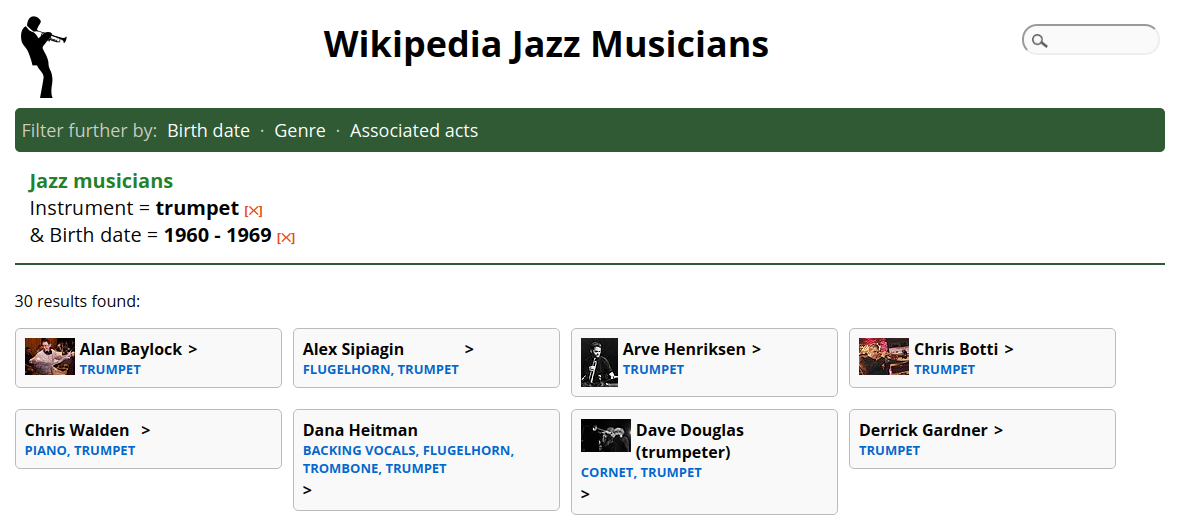
\includegraphics[width=140mm]{img/02_miga_data_viewer.png}
	\caption{Miga Data Viewer: A sample application generated from a set of Jazz Musicians.}
	\label{fig:miga-data-viewer}
\end{figure}

As we already mentioned in the introduction chapter, the big disadvantage of tabular data is that they carry very little semantic information. As without the semantic information, it would be almost impossible to generate anything else but a simple paginated table, the user is required to provide a \emph{schema definition} for each data table (for each single CSV file). That is done through configuration *.ini files using a custom \emph{Miga Data Schema} format. Here is an example of such a configuration:

\scriptsize
\begin{verbatim}
[Books]
Title = Name
Author = List (,) of Entity (Authors/Name)
Number of pages = Number
Genre = List (,) of Text
Wikipedia URL = URL

[Authors]
Name = Name
Birth date = Date
\end{verbatim}
\normalsize

Each section defines a schema for a CSV file with a name matching the section's name. Each column in the data file is assigned one of the data types provided by the \emph{Miga Data Schema}. Besides the very basic ones (\emph{Text} or \emph{Number} that correspond to data types known from programming languages) and slightly more complex ones (\emph{List} for collections, \emph{Entity} working as a \emph{foreign key} pointing to a different CSV file), there are a few special ones with added \emph{semantic meaning}. Let us name for example \emph{URL}, \emph{Image URL} or \emph{Coordinates} (GPS coordinates). Using these types the Miga Data Viewer is able to dynamically create richer interfaces (e.g. it can display entities with coordinates on a map).

It is clear that this format is the authors' attempt to solve what RDF would be perfect for. But unlike RDF, which is a universal, open and widely supported framework, this format will work with Miga Data Viewer only. We will see similar approaches in other generators as well.

Although creating an application does not require the user to know any programming language, the process does involve fairly low-level work with the *.ini schema files. Because of this we do not consider this tool \emph{non-developers friendly}.

When we ask whether this tool \emph{analyses} the data or \emph{understands} it in any way, it brings up an interesting point. In this case, it depends on whether we consider the schema to be part of the data set (as the schema is also a file, it can be distributed together with the data itself). If we do that, then we can say that the generator really \emph{understands} the data (to an extent). If it comes across GPS coordinates, thanks to the schema it will know that it is GPS coordinates, and as already explained, it will automatically add a map view to the generated application. On the other hand, if we consider the schema to be the application configuration, strictly separated from the data, then we cannot talk about any kind of \emph{understanding}. In this sense, the generator is told by the user to use a map view.

Because it is possible to put the schema and the data together, creating one package that can work as the generator input, we consider this tool to offer automatic (yet very simple) \emph{data analysis}.

\section{Citadel on the Move}

Citadel on the Move \cite{citadel_home} is a project \cite{citadel_paper} funded by European Commission. The presented goal is to simplify the process of generating Open Data 
\todo[color=green!40]{How to reference Open Data?}
based applications for both developers and non-developers, that provide useful city services. The idea behind this project was that an application providing a certain service (e.g. available park places) for one European city should be able to work just as well in another European city, only with a different data set. The applications generated by this tool are very simple map applications that work as interactive data viewers (similarly to Miga Data Viewer).

\begin{figure}
	\centering
	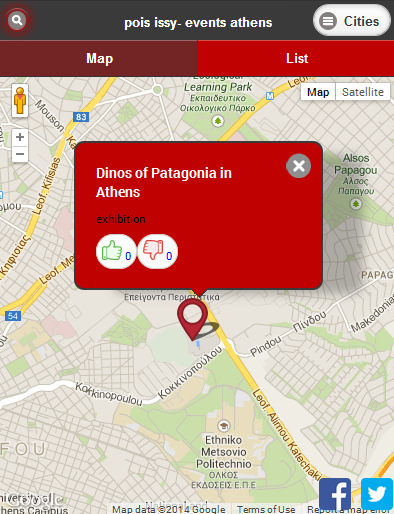
\includegraphics[width=80mm]{img/02_citadel_on_the_move_app.jpg}
	\caption{Citadel on the Move: A sample generated application. Source of picture \cite{citadel_agt_doc}}
	\label{fig:citadel-on-the-move}
\end{figure}

Citadel on the Move is not a monolithic application but a fairly large project consisting of several components.

\begin{itemize}
\item The project defines its own data set format called \emph{Citadel JSON}. As the name suggests, the data are serialized into JSON following a custom schema. Each data set contains a single list of entities where each entity has couple of mandatory fields (like a unique identificator, name or GPS coordinates necessary for the map visualization) plus an arbitrary number of optional attributes (which may vary depending on a data set and are not in any way defined by the schema). 
\item The project offers a \emph{Citadel table to JSON Converter tool} which allows the user to convert any tabular data (typically CSV or Microsoft Excel spreadsheet) into the internal \emph{Citadel JSON} format. Clearly, the original data set has to contain all required information. The tool just enables the user to create mappings between table columns of the original data set and the schema fields.
\item The core component is the \emph{Application Generator Tool} which allows non-developers to create their own applications in just couple of simple steps. They start by selecting a city (or cities) that they are interested in, they continue by selecting a data set (or data sets) available for the chosen city (or cities) and finally they just fill in basic app configuration (name, description, color scheme) to create the application. The generated application is an interactive interface that allows the user to browse, filter and see the data on a map (as said, similarly to Miga Data Viewer).
\item A part of the project is also a \emph{platform} in a form of an online portal available on the cited URL \cite{citadel_home}. It is wrapped around the  \emph{Application Generator Tool} and provides additional functionality like published applications catalog, user management, support etc.
\item The last component are customizable application \emph{templates}. If the application generated by the \emph{Application Generator Tool} is not sufficient, the user can instead manually instantiate a \emph{template} and configure it to use the given data set. This approach is completely separated from the \emph{Application Generator Tool}. It is not possible to select a template while generating an application. This has to be done manually and it requires certain programming skills. A distinct advantage is that using a template gives the user significantly bigger freedom of customization. E.g. it is possible to edit the application layout or upload a custom application logo. An example of such a special template is the \emph{Citadel Events Template} that extends the default application (which is used in the \emph{Application Generator Tool}) by a calendar which allows filtering over events contained in the data set (those are standard entities with couple extra attributes that are specified in the template documentation).
\end{itemize}

To sum it up: Citadel on the Move offers two different approaches. The first one utilizes the \emph{Application Generator Tool} which allows non-developers to generate simple applications in a very \emph{friendly} way. The other one utilizes the \emph{templates} which allow developers to create more customizable applications. There is no data \emph{analysis} involved. The user has to select a different template manually and he has to make sure that the given data set contains all necessary information that the template needs in order to work properly. The project offers several different documented templates and encourages the developers to create new ones which makes the project \emph{extendable}. As the \emph{templates} are just standalone web applications (not plugins), there is no interface that they would need to implement. However, they need to support the common \emph{Citadel JSON} format. Just like Miga Data Viewer, Citadel on the Move needs to address the problem that standalone tabular data contain almost no semantic information. To deal with that, it provides the \emph{JSON Converter tool} which allows the user to map the data set table columns onto the Citadel JSON scheme.

\section{Tableau Software}

Tableau Software \cite{tableau} is a company behind a family of professional commercial products focused on rich interactive data visualizations. The core product is Tableau Desktop. It can be used together with Tableau Server, which adds sharing, collaboration and other features useful for organizations, or with Tableau Online which is Tableau Server hosted directly by Tableau Software (i.e. cloud solution). There is also Tableau Public which offers a light-weight free version of Tableau Desktop and focuses on creating rich online public visualizations.

\begin{figure}
	\centering
	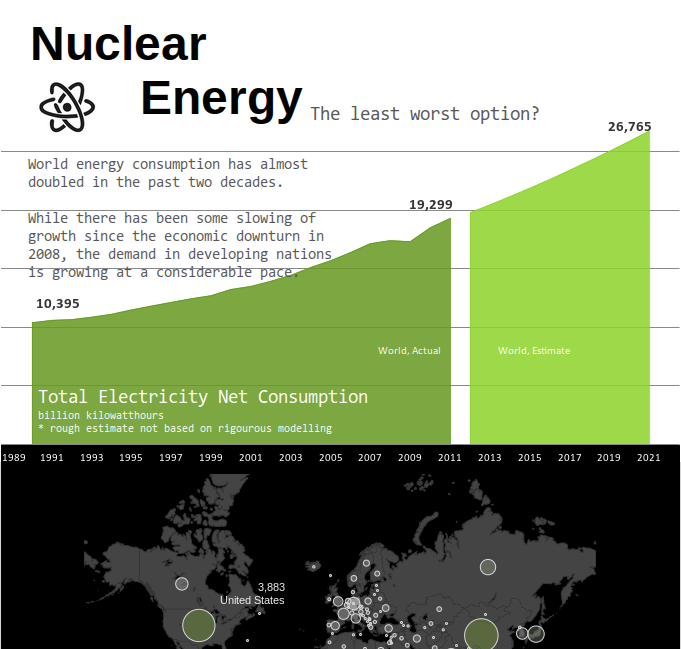
\includegraphics[width=110mm]{img/02_tableau_sample.png}
	\caption{Global Nuclear Energy Use \cite{citadel_agt_doc}. Sample rich interactive visualization created with Tableau Public}
	\label{fig:tableau-global-nuclear-enery-use}
\end{figure}

At first glance, Tableau Desktop has more in common with Microsoft Excel than with the \emph{application generators} we are describing in this chapter. A task typical for Tableau Desktop is to create a graph from a given data table. But this tool goes way beyond that. Firstly, it does not have to be just graphs. The user can choose from a very long list of rich and attractive visualizations. Secondly, the visualizations can very often be interactive, allowing easy data exploration. And lastly, multiple visualizations can exist within a single document. They can be arbitrarily combined and put into a layout chosen by the user.

A typical output of Tableau Desktop is an interactive \emph{dashboard} containing multiple visualizations. The \emph{dashboard} can be extended with filtering tools that control the underlying data set. As the end user changes the filters, the visualizations on the \emph{dashboard} change on-the-fly. The Tableau Desktop is not promoted as \emph{application generator} but given the nature of produced \emph{dashboards} it can be very well considered as one. With little effort (and with no developer knowledge) it can achieve very similar results as the previously described generators, Miga Data Viewer and Citadel on the Move.

It works only with tabular data but unlike the previous tools, it supports by default many various source types. Besides the classical ones like Microsoft Excel spreadsheets or CSV, it allows the user to connect to live databases (the published dashboards can work as live views on the database content). Tableau Desktop contains many \emph{analytical} (and statistical) tools but not in the sense that they would dynamically help the user with creating the visualizations. The process is very \emph{user-friendly} (overall drag and drop approach) but it is completely controlled by the user. The application is not really \emph{generated}, the user \emph{builds} it.

We can assume that the inner software architecture does support extending, but as it is a commercial closed source product, there is no natural way in which a user could extend the generator with features he would desire. He can only rely on the authors.

\section{Avelca}

Avelca \cite{avelca} is another commercial tool for building custom business applications. Among the tools that we are describing in this chapter, this one is probably the furthers from our original definition of a \emph{data driven application generator}. It is focused on companies and organizations allowing them to build interactive applications around their agendas. An example of an application created with this tool could be a movie rental database, keeping track of owned movies, registered customers and current rentals. Thanks to Avelca, even a user with zero developer knowledge can create such an application.

\begin{figure}
	\centering
	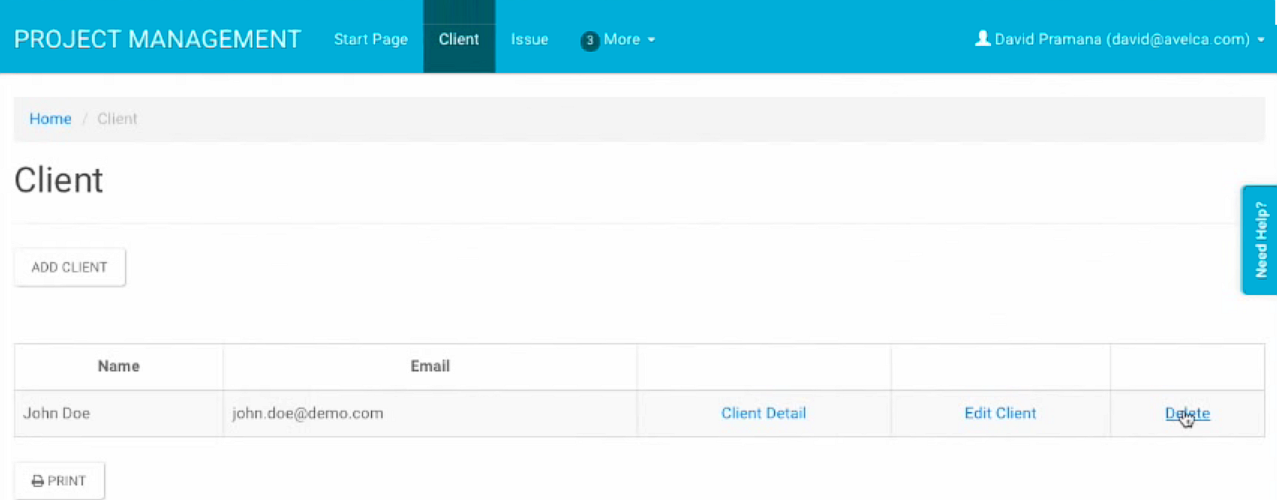
\includegraphics[width=110mm]{img/02_avelca.png}
	\caption{Sample application generated with Avelca. Source: YouTube demo video \cite{avelca_youtube}}
	\label{fig:avelca-example}
\end{figure}

In its essence, Avelca \emph{application generator} is just a \emph{user-friendly} interface over a common relational database. The user starts with creating the database schema, i.e., creating tables and defining relationships between them. Obviously, the interface is more verbose and uses vocabulary that is friendlier (it avoids the standard technical terms) in order not to scare off the non-developer user. The generator then uses the schema definition to create the actual application. Another way is to start with an existing data source (once again, only tabular data are supported, typically Microsoft Excel spreadsheet) and use it as a base for the generated application. This feature puts this tool among our \emph{application generators} but you should note that this time, starting with a data set is just an option, the user can actually begin with an empty application and use it to create the data.

Avelca is a proprietary Application Platform as a Service. That means that on one hand, \emph{online sharing} is supported by default, on the other, it is not possible to \emph{extend} the generator in the sense that we described at the beginning of this chapter. There is also no actual \emph{data analysis} going on. The application is completely built by the user. The only exception might be the situation when the tabular data are being imported and Avelca has to \emph{guess} the table schema. That process is, however, very straightforward and we can hardly speak about some kind of \emph{understanding} of the data.

In a way, Avelca is very similar to the Miga Data Viewer. Both tools work with tabular data that are augmented with a schema definition effectively turning it into some kind of relational database. The application is then generated from both the data and the schema. Clearly, Avelca is a way more advanced tool (Miga Data Viewer is just an interactive viewer) but the particular difference we are interested in at this moment, is that to achieve the same (i.e., defining the schema), they use two different approaches. Miga Data Viewer requires the user to create the schema using *.ini files, whereas Avelca offers a rich, user-friendly, drag and drop-based interface (interestingly enough, the underlying technology in Avelca uses YAML-based DSL to represent the schema).

This creates a little paradox. Miga Data Viewer \emph{feels} a bit more like an \emph{application generator} than Avelca. You start with a data set, augment it with a schema defined in a small and simple file and that is it. Miga Data Viewer generates the application from these two pieces of information. Moreover as already explained, if we consider the schema definition to be a \emph{part} of the data itself, then we can say that Miga Data Viewer actually \emph{understands} the data \emph{semantics} and uses this ability to create better and richer applications. This can be hardly claimed about Avelca. We can say that the Miga Data Viewer schema definition is part of the data only because it is an actual file that can be distributed with the data. In the case of Avelca, the schema definition is stored somewhere on the Avelca servers and the user can access it only through the user interface. It is definitely not part of the data. On top of that, the whole process of creating an application is very different and it feels more like \emph{building} than \emph{generating}. But besides all of this, the fact remains that Avelca can be used to get very similar results to what you can do with Miga Data Viewer. Avelca is like an upgraded and more advanced Miga Data Viewer with a slightly different overall approach.

We understand that his is very subjective. We are mentioning this paradox here only to show that it is hard to define and agree on what a \emph{application generator} is and that there are many different tools that might share some of the features we are interested in, but not all of them.

\section{Exhibit}

Exhibit 3.0 \cite{exhibit} is a publishing framework for large-scale data-rich interactive Web pages. It offers yet another approach compared to what we have seen so far. To see how it works, we will have a look at a sample application "Billionaires in History" \cite{exhibit_example}. The data are in Exhibit internal JSON-based format (which we will mention later) but in their nature it is just a simple 2D table containing a list of billionaires with several named properties (name, age, wealth, origin etc). The \emph{applications} produced by Exhibit are called \emph{exhibits} and they are directly embedded into HTML pages. So when creating an \emph{exhibit} like the mentioned "Billionaires in History" application, we would start with an empty HTML page. In the first step, it is necessary to link \emph{Exhibit JavaScript API} and the actual data set into the page. For this particular application, we also need to link an Exhibit plugin with the map view. Once this is done, we can start inserting Exhibit widgets and components into the HTML page using special syntax.

\begin{figure}
\centering

  \begin{verbatim}
  <div ex:role="view"
    ex:viewClass="Map"
    ex:label="Where They Are From"
    ex:latlng=".latLng"
    ex:sizeKey=".wealth"
    ex:sizeCoder="wealth-coder"
    ex:bubbleWidth="200"
    ex:bubbleHeight="200"
    ex:bubbleTip="top"
    ex:mapHeight="500"
    ex:sizeLegendLabel="Wealth in Billion USD"
    >
      <div class="map-lens" ex:role="lens" style="display: none;">
        <div>
          <b ex:content=".label"></b>
          <span ex:if-exists=".origin">
          	from <span ex:content=".origin"></span>
          </span>
        </div>
        <div><span ex:content=".wealth"></span> billions USD</div>
        <div>Company: <span ex:content=".company"></span></div>
      </div>
  </div>
  \end{verbatim}  
  \caption{Code snippet from the "Billionaires in History" application \cite{exhibit_example} showing how the map is instantiated.}
  \label{fig:exhibit-map-code-snippet}
\end{figure}

As you can see in Figure \ref{fig:exhibit-map-code-snippet}, the special syntax consists of standard HTML tags extended with custom attributes prefixed with \texttt{ex:}. We insert the map into our application by creating a new wrapping \texttt{div} tag and giving it the attributes \texttt{ex:role="view"} and \texttt{ex:viewClass="Map"}. 

The map should display a \emph{bubble} for each billionaire. The size of the \emph{bubble} corresponds to the billionaire's wealth and the position of the \emph{bubble} corresponds to the coordinates of his origin. This mapping is specified using the \texttt{ex:sizeKey} and \texttt{ex:latlng} attributes, i.e., the \texttt{ex:sizeKey} attribute says that the \emph{bubble} size should be defined by the \texttt{wealth} property, and the \texttt{ex:latlng} attribute says that the \emph{bubble} position should be defined by the \texttt{latLng} property. The child \texttt{div} with the \texttt{ex:role} attribute set to \texttt{lens} defines the looks and the contents of a \emph{bubble tooltip}  which is displayed upon a click on the \emph{bubble}. Notice how the data properties are linked to the code using the \texttt{ex:content} attribute. 

\begin{figure}
	\centering
	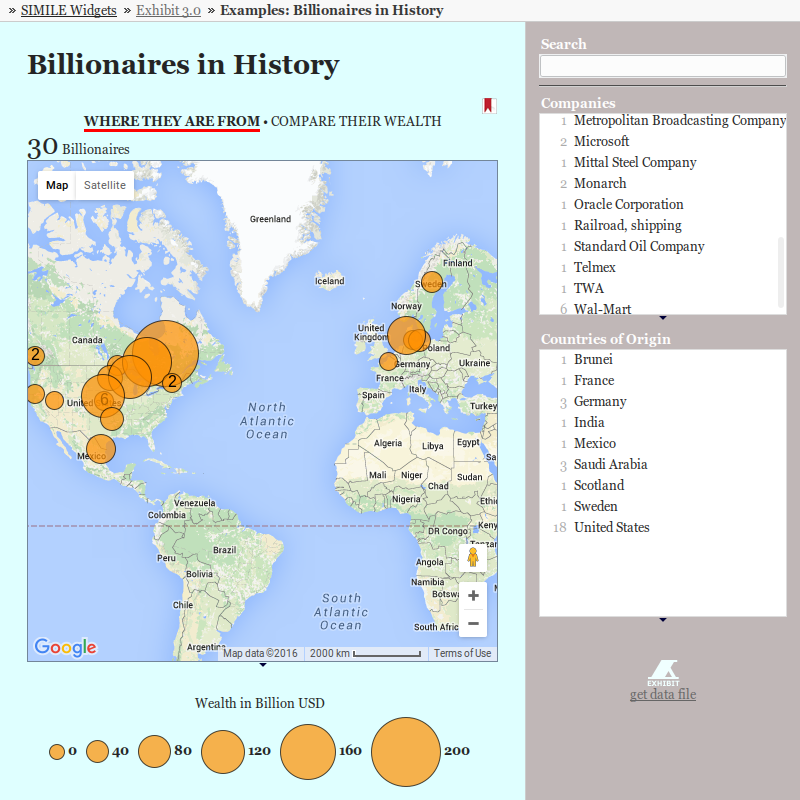
\includegraphics[width=110mm]{img/02_exhibit.png}
	\caption{"Billionaires in History" application \cite{exhibit_example} created with Exhibit.} 
	\label{fig:exhibit-map-example}
\end{figure}

Exhibit provides a large number of available components and widgets which can be used to create complex and interactive applications. As the components can be combined with standard HTML and CSS markup, the user has almost unlimited possibilities in how the final application should look like. The obvious disadvantage is that the user has to have at least some basic knowledge of HTML in order to be able to create an application with Exhibit. That means that Exhibit is not really \emph{non-developers friendly} but on the other hand, no real programming skills are needed and even with a shallow knowledge of HTML, one can achieve very good results.

In the previous cases of \emph{application generators}, we were examining how they deal with missing \emph{semantic} information. For example, Miga Data Viewer requires a schema definition which allows the user to specify the extra \emph{semantic} information. If a data property is marked as GPS coordinates, Miga Data Viewer displays the appropriate entity on a map. Exhibit has an exactly opposite approach. The user assigns the meaning to individual properties by using them \emph{properly} in component configuration. If you have a look at the map example, what happens there is that we tell the map widget that the \texttt{latLng} property contains GPS coordinates. Nevertheless, besides this approach, Exhibit does allow us to create a schema for our data as well. Typically, the schema can define how entities of different types are related to each other within a single data set.

Internally, Exhibit uses its own JSON-based data format which makes it possible for the data to live together with the schema within a single file. We have seen a similar approach with a custom format in Citadel on the Move. Just like Citadel on the Move, Exhibit also offers tools allowing arbitrary data sets to be converted into the internal format. This time, however, the internal format is way more powerful, so the original data sources are not limited to just tabular data. For example, \emph{Linked Data} are also supported by Exhibit.

As Exhibit consists of individual components and widgets, it can be naturally extended by adding new components and new widgets capable of displaying new types of data. For those who decide to extend Exhibit, there is developer documentation available \cite{exhibit_documentation}.

\section{Payola}

Payola \cite{payola} is an online all-in-one platform for reading, sharing, analyzing and visualizing LinkedData. It is a technological predecessor of another tool, LinkedPipes, on top of which our \emph{application generator} is going to be built. At first glance Payola might not look like an \emph{application generator} the way we defined it and its purpose is really slightly different, but it can be used as one.

\begin{figure}
	\centering
	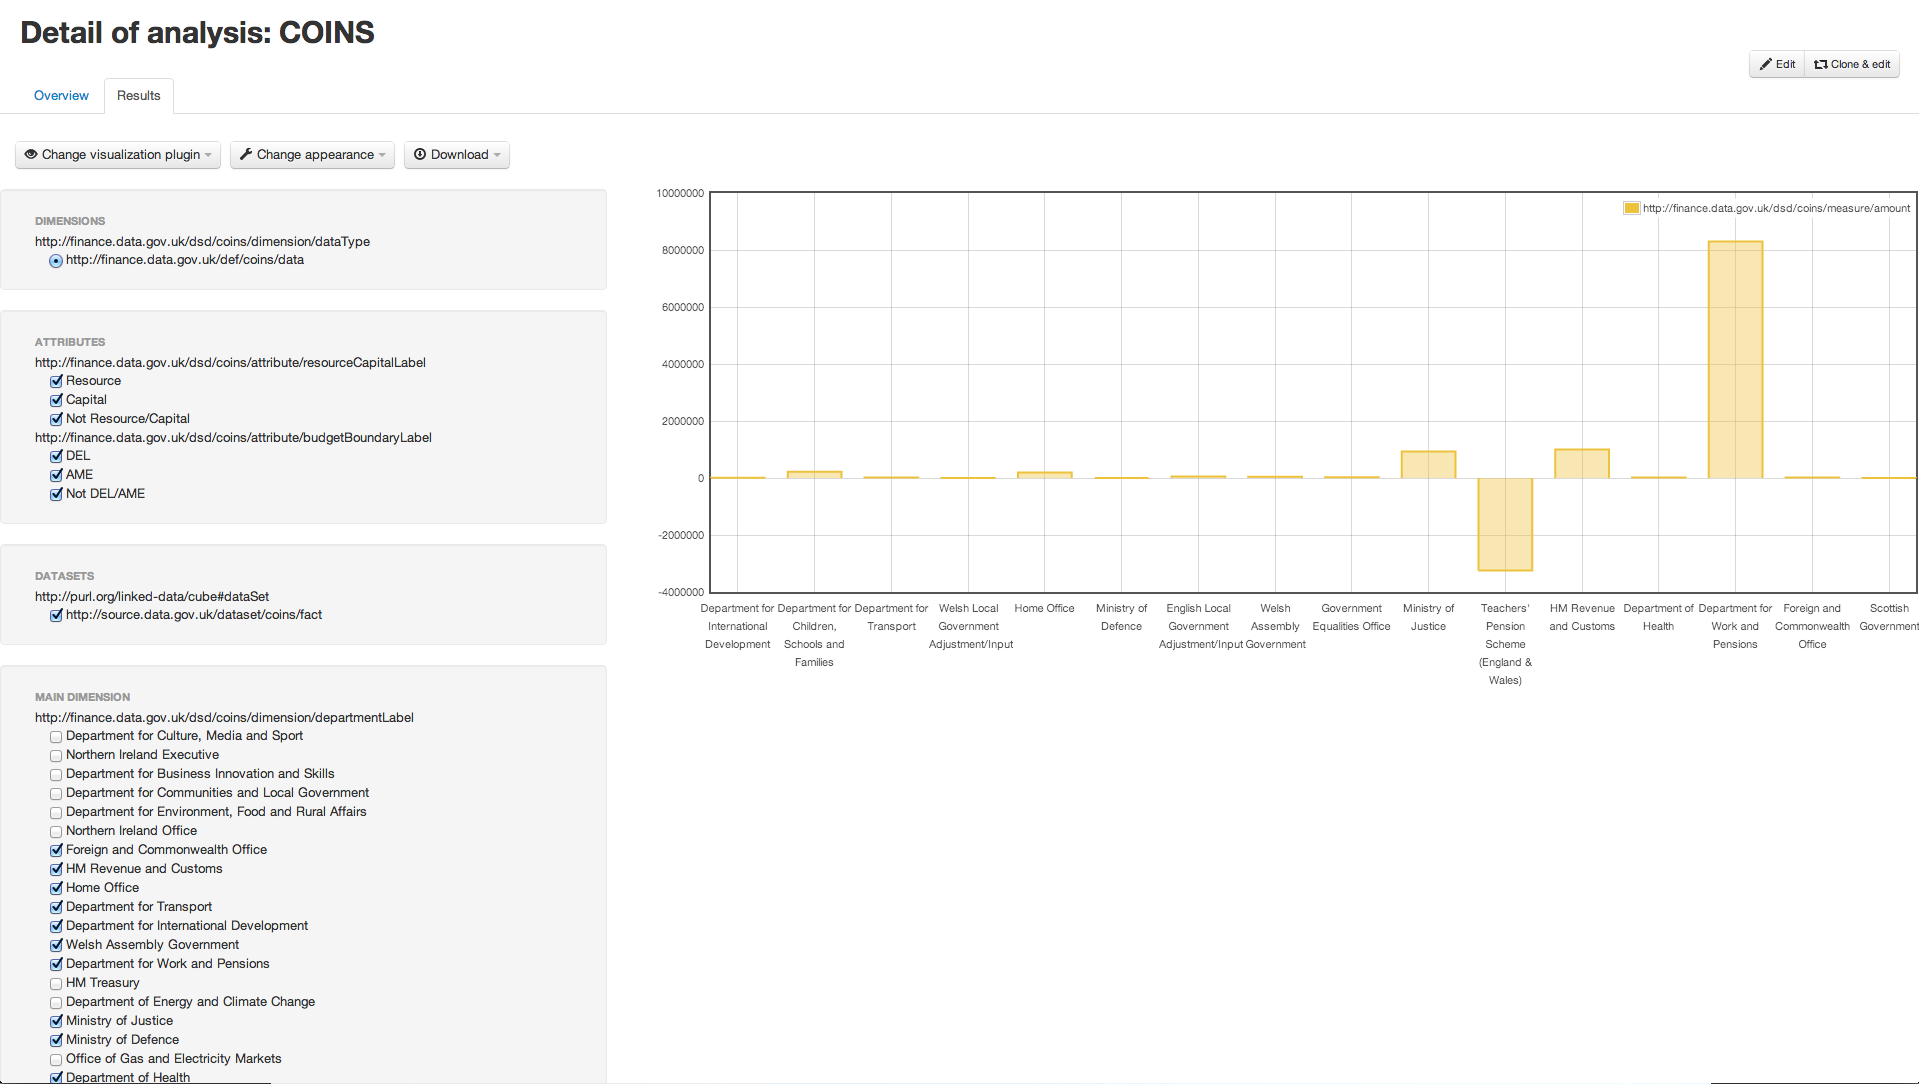
\includegraphics[width=150mm]{img/02_payola.png}
	\caption{Sample visualization created with Payola. Source: Payola User Guide \cite{payola_user_guide}} 
	\label{fig:payola-example}
\end{figure}

Using Payola, the user can build his own Linked Data \emph{analyses}. An \emph{analysis} is a hierarchical tree-like structure of plugins with a single output and multiple data inputs bound to different RDF data sources. Each plugin has an input (or multiple inputs) and it represents an operation that is applied on the input data. The idea is that the user can use the plugins to filter, search and combine the data from all the sources. By building the hierarchy of plugins, the user creates a \emph{pipeline} which can be understood as an algorithm specifying how the input data should be processed. The result of such an \emph{analysis} are also valid RDF data.

The result can be visualized using several available \emph{visualization plugins}. Some of them are interactive allowing the user to play with the \emph{analysis pipeline} output. When we talk about Payola as an \emph{application generator}, this is what we have in mind. Payola can be used to generate interactive visualizations from RDF data. The generated visualizations can be shared online using the platform features.

Unlike the previously described tools, Payola puts a lot of emphasis on the work with the data itself. All the other tools simply took the given input data source and tried to generate an application form it. Payola with its \emph{analyses}, on the other hand, leverages the distributed nature of Linked Data and offers the user a way to build his own data sources before visualizing it (that is the \emph{analysis pipeline} output). There is an interesting paradox that even though Payola allows the user to build his own \emph{analyses}, it does not perform any \emph{analysis} on its own,
\todo[color=green!40]{I hope this is a correct statement.}
i.e., it does not try to \emph{understand} the data. It is completely up to the user to explore the data, build the \emph{analysis pipeline} and apply an appropriate visualization plugin.

The final visualization is what we consider the \emph{generated application}. As such, it is not configurable in similar manner as in the previously described \emph{application generators}, i.e., it is not possible to take the \emph{analysis pipeline} output, select a visualization plugin and start building an application from it. But as the analytical process is completely controlled by the user, he can add various plugins to the \emph{analysis pipeline}, in order to alter the data output which will eventually change the visualization itself. From this perspective, the visualization can be \emph{configured} to a certain extent .

The process of creating an \emph{analysis pipeline} involves instantiating individual plugins, configuring them and binding them together. It is all done through a clickable user interface. Some basic knowledge of how Linked Data work is required, nevertheless, we would still classify the process as \emph{non-developer friendly}. On the other hand, in order to be able to perform more complex operations with the data, the user needs to be able to construct custom \texttt{SPARQL} queries.

Payola is easily extendable by new analytical and visualization plugins. The analytical plugins can be even added directly through the web interface.

\section{LinkedPipes Visualization}

LinkedPipes Visualization \cite{linked_pipes_visualization} is a successor of Payola. It is also a platform for reading, sharing, analyzing and visualizing Linked Data. As our \emph{application generator} is going to be built on top of LinkedPipes Visualization, we will dedicate one whole chapter to this tool and here we will give just a short description.

In Payola, the user has to manually build the \emph{analytical pipeline} by combining available plugins and applying them on input data sources. In LinkedPipes Visualization, the user just selects the RDF data sources and the tool will automatically discover all possible combinations of available plugins, making up \emph{pipelines} that lead to meaningful visualizations. For example, if the data set contains geospatial information, LinkedPipes Visualization will automatically offer the user a map visualization of the data. Or if the data set contains geospatial information in a format that the map visualization plugin does not understand, but there is a plugin available that can transform the data into the required format, LinkedPipes Visualization will automatically insert that plugin into the \emph{pipeline} and that \emph{pipeline} will be offered to the user.

Compared to Payola, this approach is way more \emph{non-developers} friendly and also faster as it does not involve the slow manual process of creating the \emph{analysis pipeline}. On the other hand,  the automatically generated pipeline cannot be altered or configured in any way which means that also the visualization cannot be configured. The user has to rely on the plugins that are currently available. The only way around this is to create and add a new plugin, but that is significantly more complicated and requires developer knowledge.
\chapter{LinkedPipes Visualization}
\label{chap:linkedpipes-visualization}

We already gave a brief description of LinkedPipes Visualization \cite{linked_pipes_visualization} at the end of the previous chapter. The authors state: \emph{"You point LinkedPipes Visualization to the data and it tells you what it sees in it. This way, you get to a visualization in just a few clicks."}  \cite{linked_pipes_visualization}. We will use this tool as a base for our \emph{application generator}. We will turn \emph{visualizations} into configurable interactive \emph{applications} which will push the whole concept to the next level. Before we get to how we want to achieve that and especially why we decided to use LinkedPipes Visualization in the first place, we will give the reader a deeper and more profound description of this tool. This knowledge will be required in the later parts of this text.

LinkedPipes Visualization implements Linked Data Visualization \linebreak Model~\cite{ldvm}\cite{ldvm_use_cases}. We start by describing this model as a concept, then we move on to the description of how LinkedPipes Visualization implements this model. The following section is dedicated to features of this tool in general, i.e., what it is capable of. The chapter is concluded with more technical information and implementation details of LinkedPipes Visualization.

\section{LDVM}

Linked Data Visualization Model (LDVM) \cite{ldvm} is an abstract concept that breaks down the visualization process of Linked Data into four separated stages. Those stages are \emph{Source Data}, \emph{Analytical Abstraction}, \emph{Visualization Abstraction} and \emph{View}~\cite{ldvm}. Let us walk through the individual stages.

\begin{itemize}
\item In the \emph{Source Data} stage, we begin with raw input data in an arbitrary format (it can but does not have to be in RDF). In this stage appropriate transformations need to be applied on the input data to convert them into RDF representation suitable for the next stage. For example, a CSV file could be converted into corresponding RDF representation at this stage. If the input data already are in RDF, this stage could be reduced to simple identity mapping. This transformation is done by a component which is called a \emph{data source}.
\item In the \emph{Analytical Abstraction} stage, relevant data are extracted and represented from the input produced in the \emph{Source Data} stage. Also arbitrary aggregation and computation of additional characteristics can be performed at this stage. This is typically done through a sequence of in-stage SPARQL operators. This sequence is denoted as an \emph{analyzer} component.
\item In the \emph{Visualization Abstraction} stage, the \emph{analytical abstraction} produced by the previous stage is transformed into \emph{visualization abstraction} which corresponds to the desired visualization technique. Under the hood it works very similarly to the \emph{analytical abstraction} stage as the transformation is also achieved through a sequence of in-stage SPARQL operators which is denoted as an \emph{visualization transformer} component.
\item In the final \emph{View} stage, the \emph{visualization abstraction} is transformed into an actual on-screen visualization that the user can see and potentially interact with. This visual mapping transformation is performed by a component called \emph{visualizer}.
\end{itemize}

By putting this all together, we get a \emph{pipeline} which on one end takes some arbitrary data as an input, and on the other end produces an actual on-screen visualization of the input data. If we look closely at the \emph{pipeline}, it starts with transforming the data into RDF, then follows a sequence of SPARQL operators and finally it ends with the visualization. The reason why the process is abstracted into four separate stages with four separate types of components is re-usability and composability. 

\subsection{Combining and re-using components}

Let us say we have a data set that contains a list of cities,  their populations and the countries they belong to. Clearly, all kinds of information can be extracted from such a data set. We might want to select just the cities. Or we might want to select the countries and calculate the number of cities in each country. Or we might want to select the countries and calculate the average population size of all cities in a country. For each of these tasks we would define a different \emph{analyzer}.

Now let us say we have the list of the cities and we want to visualize them on a map. Each city has GPS coordinates attached to it but unfortunately, it is using a vocabulary that our map \emph{visualizer} does not understand. In this case, we can use a \emph{visualization transformer} that converts the geospatial information into the desired format by using the supported vocabulary, i.e., it transforms the information from one vocabulary into another.

Eventually, we might actually have two different map \emph{visualizers} available, one is Google Maps based and the other one is OpenStreetMap based. Both can work with the output of the earlier mentioned \emph{visualization transformer}, i.e., they both support the same vocabulary that we converted the data set into. In other words, both \emph{visualizers} behave identically in what data they can visualize. But they differ in the actual on-screen visualization. The user can choose which one suits his need best.

The final pipeline in this example might consist of the \emph{data source}, the \emph{analyzer} that extracts the cities, the \emph{visualization transformer} that converts the geospatial information to the supported format, and eventually the \emph{visualizer} that shows the selected cities on a map.

What is important here is that every single component in this pipeline can be re-used and based on the context, it can yield different results. All kinds of other information can be extracted from this \emph{data source}. This particular \emph{analyzer} can extract cities from different \emph{data sources} and pass them on. We can easily imagine that the task of converting the geospatial data between two vocabularies, which is what our \emph{visualization transformer} does, will be pretty common. Finally, the map \emph{visualizer} can be used to visualize any geospatial data.

\subsection{Compatibility}

On top of all of this, LDVM introduces a very important concept of \emph{compatibility}. \emph{Analyzers}, \emph{visualization transformers} and \emph{visualizers} are software components that consume data through their input interfaces. What we want to know is whether an \emph{analyzer} can be applied on a \emph{data source}, whether a \emph{visualization transformer} can be applied on an \emph{analytical abstraction} and whether a \emph{visualizer} can visualize a \emph{visualization abstraction}. Strictly speaking, an \emph{analyzer} can always be applied on a \emph{data source} (and similarly in other cases), but the question here is whether it makes sense given the \emph{data source} content and the \emph{analyzer} functionality. In other words, the question is whether it will produce any results.

To achieve this, the concept of \emph{compatibility} requires that every LDVM component describes the expected format of the input data using an \emph{input signature}. The implementation details of an \emph{input signature} are not important at this moment. What matters is that thanks to \emph{input signatures} we can automatically check the \emph{compatibility} of two LDVM components, i.e., whether the output of one component can be \emph{bound} to the input of another component.

If we look back at Payola, there are many similar aspects. A Payola \emph{analysis} is also a pipeline that consists of connected \emph{plugins} that somehow process and transform the RDF data. However, there is no such thing as \emph{compatibility} in Payola. It is the user who needs to check that it is possible to combine two plugins together.

The concept of \emph{compatibility} in LDVM has two big consequences. Firstly, it is possible to automatically check that a created pipeline makes sense and can work. Secondly, it is actually possible to automatically generate a pipeline from given \emph{data source} using available LDVM components. We will describe this more in detail in the next section.

\section{LDVM implementation}
\label{sec:linkedpipes:ldvm-implementation}

The implementation of LDVM in LinkedPipes Visualization \cite{ldvm_use_cases} uses those exact four types of components defined by the model. Each component can have multiple inputs and a single output. An exception are the \emph{data source} components that have no inputs and \emph{visualizer} components that have no output. 

\subsection{Features and input descriptors}

To support compatibility, each component defines a set of its \emph{features}, where each feature corresponds to a part of expected component functionality. Using \emph{input descriptors}, a feature can define what kind of data it requires in order to be used. The implementation distinguishes between \emph{mandatory} features and \emph{optional} features. Two components are considered \emph{compatible}, if the output of the first component can be bound to one of the inputs of the second component. And that is possible only if the data on the output of the first component meet the requirements defined on that particular input by \emph{input descriptors} of all \emph{mandatory features} of the second component (note that an \emph{input descriptor} is defined by a \emph{feature} but always for a specific input).

Let us say that we have a map \emph{visualizer} with two \emph{features}. The first \emph{feature} represents the ability to display points on a map, the second one represents the ability to show labels of those points. The first one is \emph{mandatory} because without it,  we would have clearly nothing to visualize. The second one, on the other hand, can be left as \emph{optional} because without it, we still have something to show on the map. We borrowed this exact example from \cite{ldvm_use_cases}. 

Now, if we want to check the \emph{compatibility} between this \emph{visualizer} and (typically) a \emph{visualization transformer}, i.e., we want to check whether it is possible to bind the output of the \emph{visualization transformer} to the input of the map \emph{visualizer}, we can check the data produced by the \emph{visualization transformer} against the \emph{input descriptor} of the \emph{mandatory feature} to get that information. In simple words: The \emph{mandatory feature} in our example represents the ability to display points on a map. This requirement is expressed using the \emph{feature's input descriptor}, i.e., the \emph{input descriptor} says that the input data need to contain such points. So checking the \emph{compatibility} in this case actually means checking whether the output of \emph{visualization transformer} contains some points.

\subsection{Output data samples}

The last sentence in the previous paragraph suggests that in order to ensure the \emph{compatibility}, it is necessary to \emph{run} the \emph{pipeline} (i.e., apply all the SPARQL operators from all LDVM components in a pipeline on the input data) so that we get the actual data at each stage and can apply the \emph{input descriptors} on them. As the input data might be fairly large, the process of building a \emph{pipeline} could take very long.

To address this issue, the LDVM implementation in LinkedPipes Visualization requires \emph{analyzers} and \emph{visualization transformers} to provide besides the \emph{input descriptors} also an \emph{output data sample}. In order to work properly, the \emph{output data sample} should resemble the actual output of this particular component. The \emph{output data sample} should be as small as possible but at the same time as descriptive as possible (it should include all important data patterns that the component would produce).

For example, if an \emph{analyzer} produces a list of cities with their population, the \emph{data sample} should contain only one city (but with all information related to that one city). When checking the compatibility, the \emph{input descriptors} are applied on the \emph{output data sample} instead of the actual output of the previous component. That means that we do not need to run the \emph{pipeline} in order to check the compatibility. As the \emph{output data sample} is small, this checking should be fast.

Thanks to this approach, the \emph{compatibility} can be quickly checked at the design time and when we decide to \emph{run} the \emph{pipeline}, we can already be sure that all the components are at least compatible between each other.

\subsection{Component representation}
\label{sec:linkedpipes:ldvm-implementation:component-representation}

To follow the Linked Data principles, LinkedPipes Visualization implementation of LDVM represents the  components and their configuration in RDF using a custom RDF vocabulary prefixed with \texttt{ldvm}~\cite{ldvm_vocabulary_paper}\cite{ldvm_vocabulary}. That makes it possible for the LDVM components to be shared and exchanged with separate instances of LinkedPipes Visualization or possibly even with completely different LDVM based software that supports this RDF representation. This is, however, true only to an extent. Some of the components are truly transferable and independent on the actual software implementation, but many of them require to have a corresponding counterpart in the programming code (we will refer to this counterpart as to a \emph{plugin}). This applies to \emph{visualizers} (the tool actually needs to implement the visualization technique required by the \emph{visualizer} component) but also to some \emph{analyzers} or \emph{transformers} for which SPARQL operators are not sufficient.

\subsection{Discovery}

Finally, we get to the most important feature and that is automatic \emph{pipeline discovery}. LinkedPipes Visualization maintains a register of available LDVM components: \emph{data sources}, \emph{analyzers}, \emph{visualization transformers} and \emph{visualizers}. We can think of this register as of a \emph{graph}, where each component is a vertex and two components are connected by a directed edge if and only if they are \emph{compatible}. What LinkedPipes Visualization allows us to do is to select some \emph{data sources} (or add new ones). Then, it will automatically \emph{discover} (using an algorithm similar to Breadth-first search) all possible pipelines that start with selected \emph{data sources} and end with one of the available \emph{visualizers}. Note that a \emph{pipeline} is a hierarchical structure. As components can have multiple inputs, it is possible to combine the data from multiple \emph{data sources}.

\section{Features}

\subsection{Discovering visualizations}

From a \emph{non-developer} user perspective, LinkedPipes Visualization is a tool for quick and automatic visualization of arbitrary RDF data. The user simply selects a data source (or multiple data sources) and the tool returns him a list of discovered \emph{pipelines}. Each \emph{pipeline} is ended with a \emph{visualizer} which probably is the actual information that the \emph{non-developer} user is interested in. He selects one of the \emph{pipelines} and \emph{runs} it which will process all the input data according to the component definitions and finally it will produce data ready to be consumed by the \emph{visualizer}. Once this is done, the user is redirected to the actual \emph{visualization} of the produced data using the selected \emph{visualizer} component. Each such \emph{visualization} lives at a unique URL which means that it can be accessed later or shared with audience. It is also possible to embed the \emph{visualizations} into external websites.

\begin{figure}
	\centering
	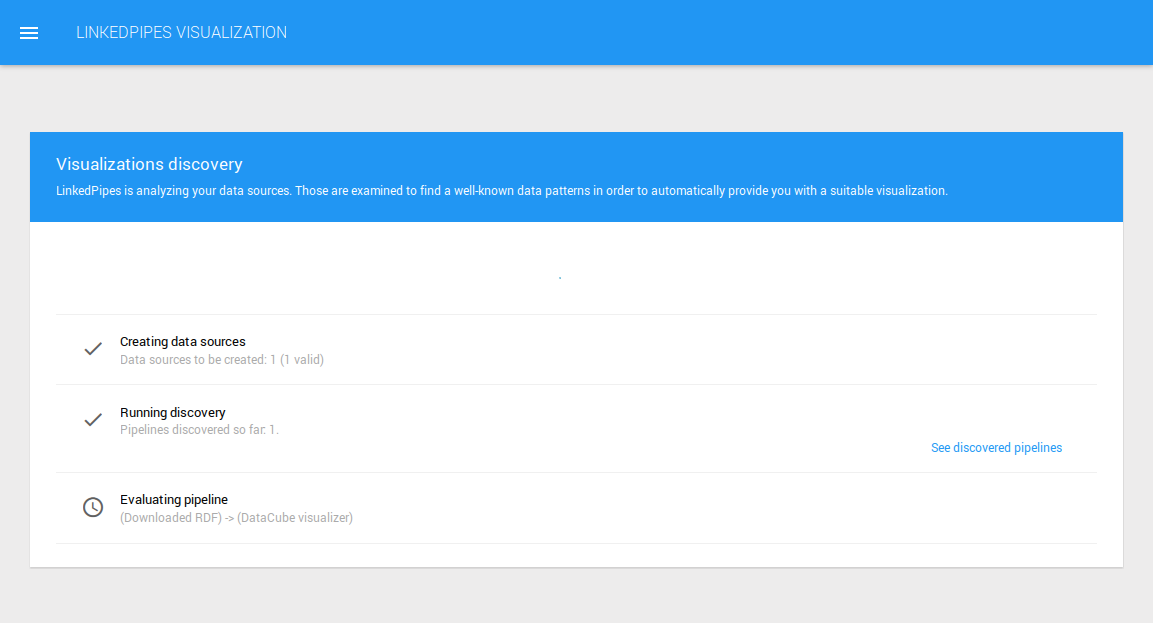
\includegraphics[width=130mm]{img/03_linked_pipes_discovery.png}
	\caption{Discovery progress in LinkedPipes Visualization} 
	\label{fig:linked-pipes-discovery}
\end{figure}

It is worth mentioning that the LinkedPipes Visualization can accept the source RDF data in many forms (following the requirements on a linked data consumption platform \cite{requirements_on_ldcp}). It can be a SPARQL endpoint, it can be a URL pointing to a file containing RDF data serialized in one of the existing formats (TTL, RDF/XML etc.) or such a file can be directly uploaded to LinkedPipes Visualization. As already mentioned, non-RDF data are not supported.

\subsection{Adding components}

More advanced users that understand RDF on a lower technical level and are capable of writing SPARQL queries, can implement and add their own LDVM components. A typical scenario might be that such a user has a new RDF data set and he wants to use one of the available \emph{visualizers} to visualize it. To achieve that, he can develop his own LDVM component, an \emph{analyzer} or \emph{visualization transformer} (or both), that converts the input data set into the format required by the \emph{visualizer}. The definition of such a component can be easily uploaded through LinkedPipes Visualization user interface. Once this is done, the new component becomes part of the register and can be used by the \emph{discovery algorithm}.

\begin{figure}
	\centering
	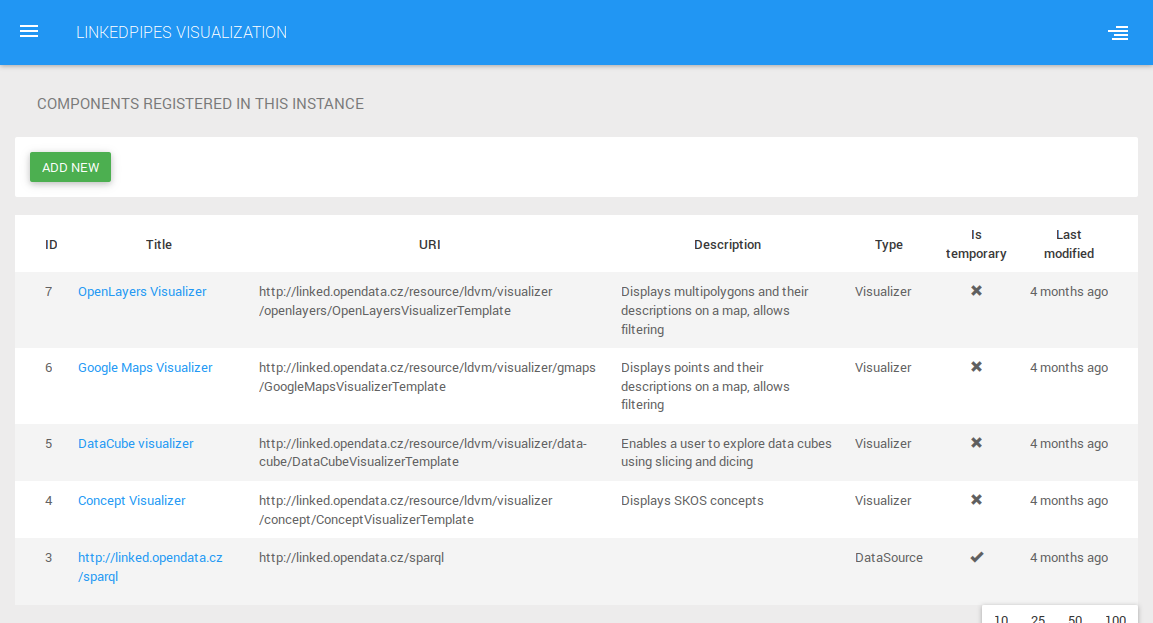
\includegraphics[width=130mm]{img/03_linked_pipes_components.png}
	\caption{Overview of available registered LDVM components in LinkedPipes Visualization} 
	\label{fig:linked-pipes-components}
\end{figure}

Users with actual developer skills can extend LinkedPipes Visualization with new \emph{visualizers} and more advanced \emph{analyzers} and \emph{visualization transformers}. That involves developing both the RDF definition using the \texttt{ldvm} vocabulary and the corresponding \emph{plugin} in programming code. 

\section{Implementation}

In the next section we will give the reader an overview of the inner architecture and used technologies. We will especially focus on how \emph{visualizers} work as those will essentially be our \emph{generated applications}.

\subsection{Architecture}
\label{sec:linkedpipes:architecture}

LinkedPipes Visualization is a web application that consists of a backend running on a server and a frontend running on the client side (in a web browser). 

The frontend is a so called Single-page application (SPA). That means that the application user interface lives completely in the browser and uses asynchronous HTTP requests (AJAX) to communicate with the backend. There are no page reloads or transitions between different pages with different URLs. That is all handled by the SPA within a single page. The data between the server and the client are sent serialized to JSON.

To be more accurate, LinkedPipes Visualization actually consists of several SPAs, each dealing with a different task. Visualization is one SPA, component management is one SPA and each visualizer is also one SPA. The frontend is driven by the JavaScript framework AngularJS\footnote{\url{https://angularjs.org/}} and the interface is created using modern web technologies, specifically HTML5 and CSS3. Several other JavaScript libraries are used as well (for example D3.js~\cite{d3js} for creating rich visualizations).

The backend is developed in Scala using Play Framework. This framework follows MVC architecture, nevertheless in this case the \emph{View} layer is significantly suppressed as its work is done by the thick client. The tool uses H2 relational database\footnote{\url{http://www.h2database.com/}} to persist arbitrary application data, and the triplestore Virtuoso\footnote{\url{http://virtuoso.openlinksw.com/}} as a private RDF data storage (that is required, for example, when evaluating \emph{pipelines}). Figure \ref{fig:linked-pipes-visualization-architecture} shows the overall architecture of Linked Pipes Visualization, including the data flow between individual layers.

\begin{figure}
	\centering
	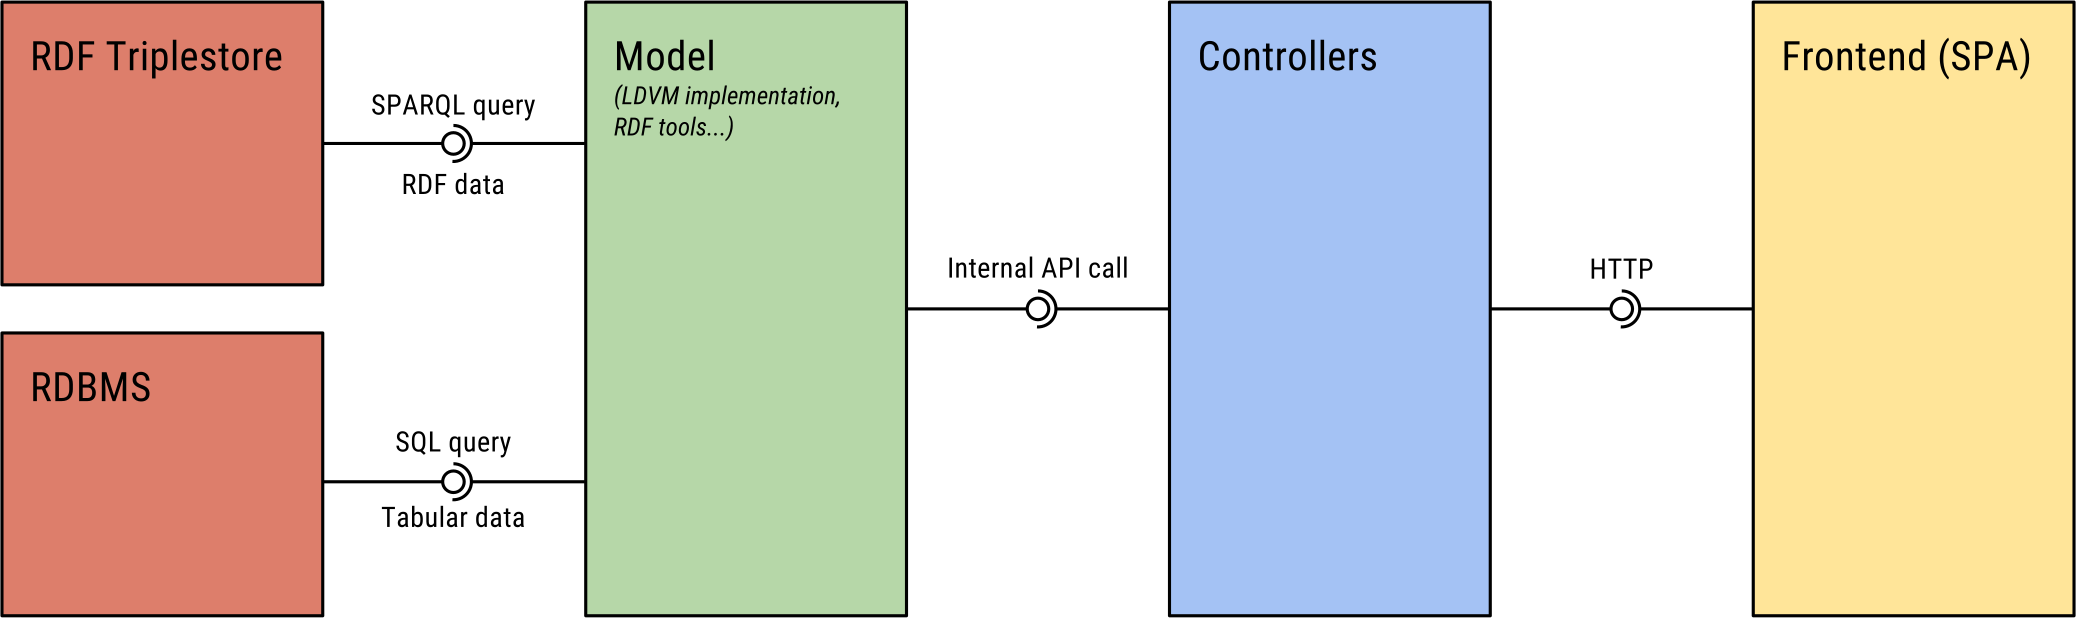
\includegraphics[width=140mm]{img/03_linked_pipes_visualization_architecture.png}
	\caption{Linked Pipes Visualization Architecture.}
    \label{fig:linked-pipes-visualization-architecture}
\end{figure}

\subsection{Component registration}
\label{sec:linkedpipes:component_registration}

We mentioned that if the user uploads a definition of a new LDVM component, it is added to the \emph{register}. What actually happens under the hood is that such a component gets inserted into the H2 database where it can be easily accessed during the \emph{discovery}. We also mentioned that some LDVM components require to be accompanied by a complementary \emph{plugin} in the code.

Let us start with \emph{analyzers} and \emph{visualization transformers}. These components perform transformations on the RDF data. Typically, this is done using SPARQL operators but sometimes that is not enough and the transformation needs to be implemented using an actual programming language (Scala in this case). The backend code contains a simple \texttt{switch} that defines which snippet of code should be executed for which component (the \emph{snippet} is actually a well-defined \emph{plugin} implementing given plugin interface). Here we would like to remind the reader that components are defined and represented in RDF using the \texttt{ldvm} vocabulary. That means that each component is actually an RDF resource with a unique URI. This URI is used in the \texttt{switch} to identify the components. 

So if a user wants to create such a component, firstly, he needs to create the RDF definition of that component and upload it, secondly, he needs to develop the plugin doing the actual component work (the data transformation), and lastly, he needs to add the component to the aforementioned \texttt{switch}. 

The situation is very similar for \emph{visualizers} as well. Each visualizer is a standalone SPA that lives on a unique URL. When the evaluation of a \emph{pipeline} finishes, the user needs to be redirected to this URL. So just as there is a \texttt{switch} defining which plugin corresponds to which \emph{analyzer} (or \emph{visualizer}), there is a \texttt{switch} defining which URL corresponds to which \emph{visualizer} (a \emph{visualizer component} is also identified by a URI).

\subsection{Visualizers}
\label{sec:linkedpipes:visualizers}

As already explained, a \emph{visualizer} is a standalone SPA that lives on a unique URL within LinkedPipes Visualization web application. Part of this URL is a parameter which specifies the \emph{pipeline} output that should be visualized using this \emph{visualizer}. The output (or more correctly the \emph{pipeline evaluation}) is a named graph stored in the private triplestore. Each \emph{pipeline evaluation} is also represented by a record in the H2 database and this record contains the graph name. The numeric \texttt{id} of this record is passed through the aforementioned URL parameter. We can say, in this sense, that a \emph{visualizer} is a function that takes the \emph{pipeline evaluation} \texttt{id} as an argument and returns the actual \emph{visualization}.

A typical workflow of a \emph{visualizer} is that once the SPA is loaded, it starts making asynchronous HTTP requests to the backend to fetch the data that should be visualized. The requests are translated by controllers into API calls to the \emph{Model} layer.  The \emph{Model} layer converts API calls into SPARQL queries that fetch data from the named graph which is stored in the private triplestore and contains the \emph{pipeline evaluation}. The returned RDF data are extracted into a representation of native objects and eventually converted to JSON and sent back to the client where they are visualized for the user (see Figure \ref{fig:linked-pipes-visualization-architecture}).

The \emph{pipeline evaluation} might be too large or it still might not be in the proper format for the chosen visualization technique. It is a responsibility of a \emph{visualizer} to deal with these potential problems and that might require some more transformations along the way. Those can be done both on the client side and the server side, whichever way is more suitable. It is not always possible to send the whole data set directly to the client and it has to be somehow reduced on the server side. A typical example of such reduction is that the \emph{visualizer} lets the user apply some filters first. That means that it (ideally) never fetches (and visualizes) the whole data set at once but always only a subset specified by the user. 
\chapter{System proposal}
\label{chap:system-proposal}

Based on the information we gathered in the previous chapters, we will now propose our own \emph{application generator}. We will give a detailed description and justification of the characteristics and features that our system will have. 

At the beginning of the chapter covering Related Work (Section \ref{sec:rw:definition}), we attempted to define what a \emph{data-driven application generator} is. We admitted that this definition is rather vague and subjective but it is important because it gives as a starting point for making our own tool of this kind. We will now briefly repeat that definition.

A \emph{data-driven application generator} is a tool that takes an input data set provided by the user and produces an \emph{application} based on that data set. Defining an \emph{application} is rather difficult. For us, the main aspect is \emph{interactivity}, i.e., the generated \emph{application} will let the user interact in some way with the source data set. Moreover, a generated \emph{application} should be persistent and to an extent independent on the \emph{generator}. When the \emph{generator} is closed, the \emph{application} should not seize to exist.

\section{Proposed features}
\label{sec:proposal:features}

In Section \ref{sec:rw:features}, we presented a list features that we focused on when examining individual related tools. This list of features allowed us to compare the tools between each other in a more organized way. This list also contains the exact features that we would like our tool to have. Let us walk through that list again and explain why we think our \emph{application generator} should support these features.

\begin{itemize}
\item \emph{Linked Data support}. The majority of the examined tools supported only some kind of tabular data. That proved itself to be a very limiting factor. Each tool required the user to somehow provide the missing \emph{semantic} information (e.g. by describing the data using a \emph{schema}) and even then the tool either generated applications that looked all more or less the same (Miga Data Viewer, Citadel on the Move), or required the user to manually build the whole application (Tableau, Avelca, Exhibit). Linked Data carry way more \emph{semantic} information with them and can be \emph{understood} by the \emph{application generator}. That means that the process of generating applications can be automated (the user does not have to explain to the \emph{generator} what the input data mean) and also as the Linked Data can express way more kinds of information, way more types of applications can be generated from that data.
\item \emph{Extendability}. All applications generated for example by Miga Data Viewer looked more or less the same.  This is caused to a large extent by the characteristics of the tabular data. Linked Data, on the other hand, are way more versatile, potentially allowing way more versatile applications. Also we can hardly imagine that we could come up with a universal solution that would work for any type of data. Therefore making the \emph{generator} extendable with new types of applications for different types of data is a necessity.
\item \emph{Data analysis}. A \emph{generator} that automatically analyzes the input data and makes decisions based on how it \emph{understands} the data, is definitely a more capable \emph{generator}. This is directly related to the \emph{Linked Data support}. It is the Linked Data that allow such analysis possible (we are not claiming that it is not possible to run some kind of smart analysis on tabular data, but as it would involve lots of guessing, the results might be debatable). Just to repeat what we have already said: such a smart \emph{application generator} can significantly speed up the process of application generation by making it \emph{semi-automatic} and it can support significantly more types of information with significantly more types of applications.
\item \emph{Online sharing}. Being able to \emph{share} the final generated application with others is the purpose of all these efforts. We aim to use the whole potential of the data around us and keeping our findings just to ourselves would clearly waste that potential.
\item \emph{Non-developers friendly}. Miga Data Viewer or Exhibit proved that even tools that require their users to have some programming skills, can help a lot by reducing the amount of work necessary for generating an application. Also these tools typically offered a high level of flexibility. Nevertheless, most of our potential users have zero developer skills and we would like to allow these users to generate applications using our \emph{application generator}.
\item \emph{Platform}. Tools in the form of an online platform (Avelca, Tableau, Citadel on the Move, Payola) clearly make the whole agenda around applications (creating, managing, sharing) simpler for the user. We want our tool to work as a platform as well.
\item \emph{Configuration}. We have seen two extremes among the examined tools. LinkedPipes Visualization simply produced the visualization and gave user no possibility to configure it before publishing. Tools like Tableau, Avelca or Exhibit, on the other hand, represented the other extreme. The user had to actually \emph{build} the whole application from scratch. Miga Data Viewer was somewhere in between. Most of the application was automatically generated but the user was still allowed to change certain aspects. This is the way that we would like to choose for our \emph{application generator} as well. We want to find a compromise solution that would allow the user to quickly generate new applications and yet it would still give him some space to influence how the application should look like before it gets published.
\end{itemize}

\section{Advantages and disadvantages of integration into LinkedPipes Visualization}
\label{sec:system_proposal:integration}

We proposed that some kind of \emph{data analysis} should be a part of our \emph{application generator}. Automatic analysis of Linked Data, however, is a vast topic. Within the scope of this thesis, we would be probably able to come up only with a very basic solution consisting of simple rules such as  \textit{"This entity is an address or GPS coordinates, let us display it on a map."} or \textit{"These are some statistical data, let us visualize it using a graph"}. We can say that Miga Data Viewer works in similar way.

We believe that it is not always necessary to reinvent what has been already invented and that we would rather give ourselves a head start by re-using an existing solution. For various reasons, we decided to integrate our \emph{application generator} into LinkedPipes Visualization. Let us now walk through those reasons.

\begin{enumerate}
\item Through LinkedPipes Visualization we get a strong analytical framework that we can immediately use. We will utilize the \emph{discovery} algorithm which will automatically tell use how the input data can be visualized, i.e., what kinds of applications can be generated.
\item We will greatly benefit from the LinkedPipes Visualization implementation of LVDM. Firstly, it will make our generator easily extendable to support new types of data through new LDVM components. Secondly, any LDVM component following the format defined by this implementation will automatically work in our generator as well (with the limitations explained in Section \ref{sec:linkedpipes:component_registration}).
\item On a programming level, LinkedPipes Visualization already contains lots of ready-to-use solutions for working with RDF data (querying Virtuoso triplestore, converting RDF to JSON etc.). It also offers a programmatical API providing a direct access to the \emph{discovery} algorithm (launching, accessing results etc).
\item Finally, we admit that what played an important role in our decision process was the fact that we had direct personal access to the authors of LinkedPipes Visualization. That significantly sped up our work.

\end{enumerate}
This decision has also disadvantages. The original guidelines for this thesis suggest that the user should be able to combine together different views for different types of data. Such views should be possible to display in a selected predefined layout before publishing the app. We have seen this approach for example in Tableau. However, LinkedPipes Visualization visualizers use a completely different approach. They are typically very domain specific. Each visualizer focuses on a single type of data, for example map data, and then offers a rich (but static) user interface which is specifically designed to work with this particular type of data (for example, it displays controls allowing the user to filter the visualized data). This is a direct consequence of the underlying LDVM pipeline \emph{discovery} algorithm.

Unfortunately, if we are to build on top LinkedPipes Visualization, our applications (which will directly correspond to the \emph{visualizers}) cannot look and work much differently. Nevertheless, both approaches are viable and both have their advantages and disadvantages. By adopting the approach of domain-specific applications, we will reduce the application configurability and it will not be possible to generate dashboard-like applications known from Tableau. On the other hand, our domain-specific applications will offer richer user interfaces allowing more advanced work with the visualized data.

\section{Contribution}

We already classified LinkedPipes Visualization as an \emph{application generator} when we were comparing related tools. The reader might ask how exactly is our \emph{application generator} going to be better. 

\subsection{Configuration phase}

In LinkedPipes Visualization, when the user selects and executes a \emph{pipeline}, he is redirected to the corresponding \emph{visualizer} user interface. That generates the actual \emph{visualization} from the \emph{pipeline evaluation}. In the context of LinkedPipes Visualization, that is the generated application. In our \emph{application generator}, we will introduce a configuration phase that will precede the publication. Each \emph{visualizer} will consist of two user interfaces: a \emph{configurator} interface and an \emph{application} interface. 

The \emph{configurator} interface will let the user to shape the application before publishing. The configuration possibilities will differ depending on the \emph{visualizer}, but typically the user will be allowed to filter the data (select a subset) and tune the level of interactivity for the audience. For example, he could either create a completely static visualization with pre-filtered data (e.g. a static graph), or he could let the audience decide what they want to see (i.e., let the audience decide what kind of graph they want to see). This will greatly increase the re-usability of data sets and \emph{visualizers}. A single data source with a single \emph{visualizer} will work as a potential source for many applications, each serving a different purpose (and a different target audience).

The \emph{application} interface is what the end-user (the audience) is going to see. When describing how a \emph{visualizer} works in LinkedPipes Visualization (Section \ref{sec:linkedpipes:visualizers}), we stated that a \emph{visualizer} is a function that takes the \emph{pipeline evaluation} as an argument and returns the actual \emph{visualization}. In our \emph{application generator}, the \emph{application} interface will be a function with two arguments: the \emph{pipeline evaluation} and the configuration created in the \emph{configurator}.

By introducing the configuration phase, we created another level of abstraction. The process of generating a new application (which includes the configuration phase now) requires no programming skills. It is very \emph{non-developer friendly}. But it does require certain understanding of the data. Not to mention that the data produced by the \emph{pipeline} might not be in a perfect state and therefore making sense out of the data (e.g. creating a meaningful graph) might require quite a lot of effort. In LinkedPipes Visualization, any user has to put in this effort when using the generated \emph{visualization}. In our \emph{application generator}, only the user generating the application will have to make this sacrifice while in the configuration phase, but the end user (the audience) will get only the final refined application.

We should mention that some features will be available in all \emph{configurators} regardless of the \emph{visualizer}. The user will be allowed to fill missing information (e.g. missing labels) and provide basic application meta data (name and description).

We should also eliminate any confusion in the terminology that might have arisen in this section. A \emph{visualizer} is the last LDVM component in a \emph{pipeline}. It consists of the RDF definition and of the actual implementation in the code (the \emph{plugin}). The RDF definition is always the same, but the  \emph{plugin} will differ for LinkedPipes Visualization and of our \emph{application generator}. In the latter case, a \emph{visualizer} will consist of the aforementioned \emph{configurator} interface and \emph{application} interface. In a sense, it will work as an \emph{application template} for generating new applications. Nevertheless, we will stick to the term \emph{visualizer} in the rest of this text.

\subsection{Platform}

LinkedPipes Visualization is a technical successor of Payola but it dropped most of Payola's platform features along the way. We will give them back, at least to the extent that makes sense for our cause. As our applications will be configurable, we will build an agenda around application management. That includes also support for registering and authenticating users.

Moreover, one of the Payola's important features was sharing and re-using of the \emph{plugins}. This also works in LinkedPipes Visualization. The \emph{discovery} algorithm is using all available LDVM components. But when a user wants to specifically run the \emph{discovery} algorithm on a \emph{data source} that already exists in the system, it is not possible. We will make a simple database of available data sets part of our \emph{application generator}. The idea is that some users will be responsible for producing interesting data sets and the platform will allow them to share the data sets with other users who will use them to generate applications. Also a simple catalog of published applications will be part of the platform.

In general, the whole user interface of LinkedPipes Visualization is rather bare and simplistic as its point is merely to show the capabilities of the underlying LDVM \emph{discovery} algorithm. Our aim, on the other hand, will be to create a more refined and polished product. Obviously, this aspect is rather subjective and we will let the reader to be the judge of that.

\subsection{Framework}

In Section \ref{sec:linkedpipes:component_registration} we described how new LDVM components  can be integrated into the code of LinkedPipes Visualization. As this tool defines a clear way how it can be extended, we can say it also fits into the role of a framework for implementing new types of Linked Data visualizations. Also when we were talking about the advantages and disadvantages of integrating our generator into LinkedPipes Visualization (Section \ref{sec:system_proposal:integration}), we mentioned that on a programming level, we will be able to utilize various available APIs for working with RDF data. Unfortunately, LinkedPipes Visualization offers no such help for development of the \emph{visualizer} user interface.

Our \emph{visualizers} are different. In front of all, they are more complicated because they consist of two different user interfaces, the \emph{configurator} and \emph{application}. The framework will have to define a clear way how to seamlessly integrate both of these interfaces into the generator.

We will define a recommended structure for the \emph{configurators} which will speed up their implementation. Thanks to this unified structure, it will be possible to leverage ready-to-use solutions for some common tasks, e.g. saving and loading the application configuration, universal support for multiple languages and adding/editing labels of RDF data. On the server side, we will provide a universal persistent request cache to increase the performance of published applications. None of these features are currently available in LinkedPipes Visualization.

Naturally, thanks to the framework, the user will not have to deal with any of the platform related tasks (e.g. authentication or authorization) and the platform features will be provided to him via explicit API (e.g. access to currently authenticated user).

\section{Visualizers}

To showcase the capabilities of our \emph{platform} and \emph{framework}, we will implement and present to the user two \emph{visualizers}. The first one will be a brand new D3.js Chord Visualizer based, as the name suggest, on the D3.js chord layout, capable of visualizing directed weighted graphs. The other one will be based on the existing LinkedPipes Visualization map visualizer. The RDF definition will remain the same, we will just re-implement the \emph{visualizer} for our \emph{application generator}.

\section{Mockups}

In this subsection we will briefly present to the reader our idea of  the \emph{application generator} user interface. The core parts are the process of generating a new application and configuring an existing application. Let us start with generating an application.

In the first step (Figure \ref{fig:mockups_select_datasources}), the user has to select the RDF data sources. Unlike LinkedPipes Visualization, our \emph{application generator} will offer a user-friendly browser of available data sources (the \textbf{Browse} button on Figure \ref{fig:mockups_select_datasources}) which means that the user will not be forced to deal with notions like SPARQL endpoint, named graph or TTL file. On the other hand, the more advanced users will be allowed to add their own RDF data sources (the \textbf{Add new} button).
\begin{figure}
	\centering
	\includegraphics[width=140mm]{img/04_mockups_select_datasources.png}
	\caption{Step 1: Selecting data sources. The user is allowed to select an arbitrary number of data sources, either from the already available ones using the browser, or by providing new ones.} 
	\label{fig:mockups_select_datasources}
\end{figure}
\begin{figure}
	\centering
	\includegraphics[width=140mm]{img/04_mockups_discovery.png}
	\caption{Step 2: Running \emph{discovery} algorithm. The screen shows current progress including already discovered \emph{pipelines}.} 
	\label{fig:mockups_discovery}
\end{figure}

Once the user is happy with his selection, he hits the \textbf{Run Discovery} button and is redirected to the next screen (Figure \ref{fig:mockups_discovery}) where he can watch the progress of the \emph{discovery} algorithm. As new \emph{pipelines} are discovered, they are shown on the screen, grouped by their LDVM \emph{visualizer} component. That means that unlike in LinkedPipes Visualization, the user can easily see what kinds of visualizations (or applications) are possible from selected data sources. The user first decides for a \emph{visualizer} and then clicks the appropriate \textbf{Show pipelines} button (Figure~\ref{fig:mockups_discovery}) which will open a list of discovered \emph{pipelines} for the chosen \emph{visualizer}.

\begin{figure}
	\centering
	\includegraphics[width=140mm]{img/04_mockups_configurator.png}
	\caption{Sample \emph{configurator interface}. The upper part is for all \emph{visualizers} identical, covering common functionality, the lower part is custom. In this case, the application visualizes entities on a map.} 
	\label{fig:mockups_configurator}
\end{figure}

Now the user selects one of the discovered \emph{pipelines} and executes it which will process the data from the data sources and transforms them (according to the \emph{pipeline} structure). This might take a while. Once the \emph{pipeline evaluation} finishes, the user can create a new application from it. Unfortunately, we are not able to help the user in any way with choosing a \emph{pipeline}. If there are multiple \emph{pipelines} available for a single \emph{visualizer}, the user might have to try all of them to see which gives him the best results.

When an application is created, the user is taken to the \emph{configurator} interface (Figure \ref{fig:mockups_configurator}) where he can modify the application before it gets eventually published.

\section{Architecture analysis}
\label{sec:system-proposal:architecture-analysis}

We decided that we would build our \emph{application generator} on top of LinkedPipes Visualization (Section \ref{sec:system_proposal:integration}). We already described the architecture of this tool (Section \ref{sec:linkedpipes:architecture} and especially Figure \ref{fig:linked-pipes-visualization-architecture}). We will now describe the way the \emph{application generator} is integrated into LinkedPipes Visualization, including the overall software architecture.

\subsection{Integration into LinkedPipes Visualization}

There were two basic ways how we could approach the integration:

\begin{enumerate}
\item Make the \emph{application generator} a part of LinkedPipes Visualization, i.e., directly integrate the \emph{application generator} into the codebase.
\item Develop the \emph{application generator} as a separate application and use an instance of LinkedPipes Visualization as a service providing required functionality via a remote (HTTP) API.
\end{enumerate}

As of the second approach, the architecture of LinkedPipes Visualization (Figure \ref{fig:linked-pipes-visualization-architecture}) would be well suited for it. The backend of LinkedPipes Visualization exposes its functionality (including the LDVM implementation) to the frontend via a public HTTP API. We could immediately use that API in our \emph{application generator}. In general, this would be the cleanest approach from the software architectonic perspective.

Unfortunately, it turned out that if we used LinkedPipes Visualization as a separate service, we could not avoid changes in the codebase of LinkedPipes Visualization. Consider, for example, how a \emph{visualizer} works (see Subsection \ref{sec:linkedpipes:visualizers} for the complete workflow). An important part of a \emph{visualizer's} job is to take the \emph{pipeline} output (which is in RDF) and convert it into a format suitable for the visualization itself (typically JSON). This conversion routine would clearly differ for each \emph{visualizer} as each \emph{visualizer} would be dealing with different kind of data. In LinkedPipes Visualization, this happens on the backend, i.e., each \emph{visualizer} exposes its own public API providing the data extracted from RDF in JSON. The consequence for us is pretty clear: if we wanted to extend our \emph{application generator} to support another type of RDF data, i.e., add another \emph{visualizer}, we would need to extend LinkedPipes Visualization as well. 

A possible solution to this problem would be to alter the public API of LinkedPipes Visualization to return the original RDF data instead and move this custom \emph{visualizer} functionality (we referred to it as to a \emph{plugin}, see Subsection \ref{sec:linkedpipes:ldvm-implementation:component-representation}) to the \emph{application generator}. Working with RDF, however, is a bit complicated and the codebase of LinkedPipes Visualization already contains several ready-to-use solutions that, among other things, significantly speed up the process of implementing support of new types of RDF data (new vocabularies). We could surely use those solutions in our \emph{application generator} but to make them available there, we would need to transfer them somehow (i.e., duplicate) or come up with a way how to share them between the \emph{application generator} and LinkedPipes Visualization.

\begin{figure}
	\centering
	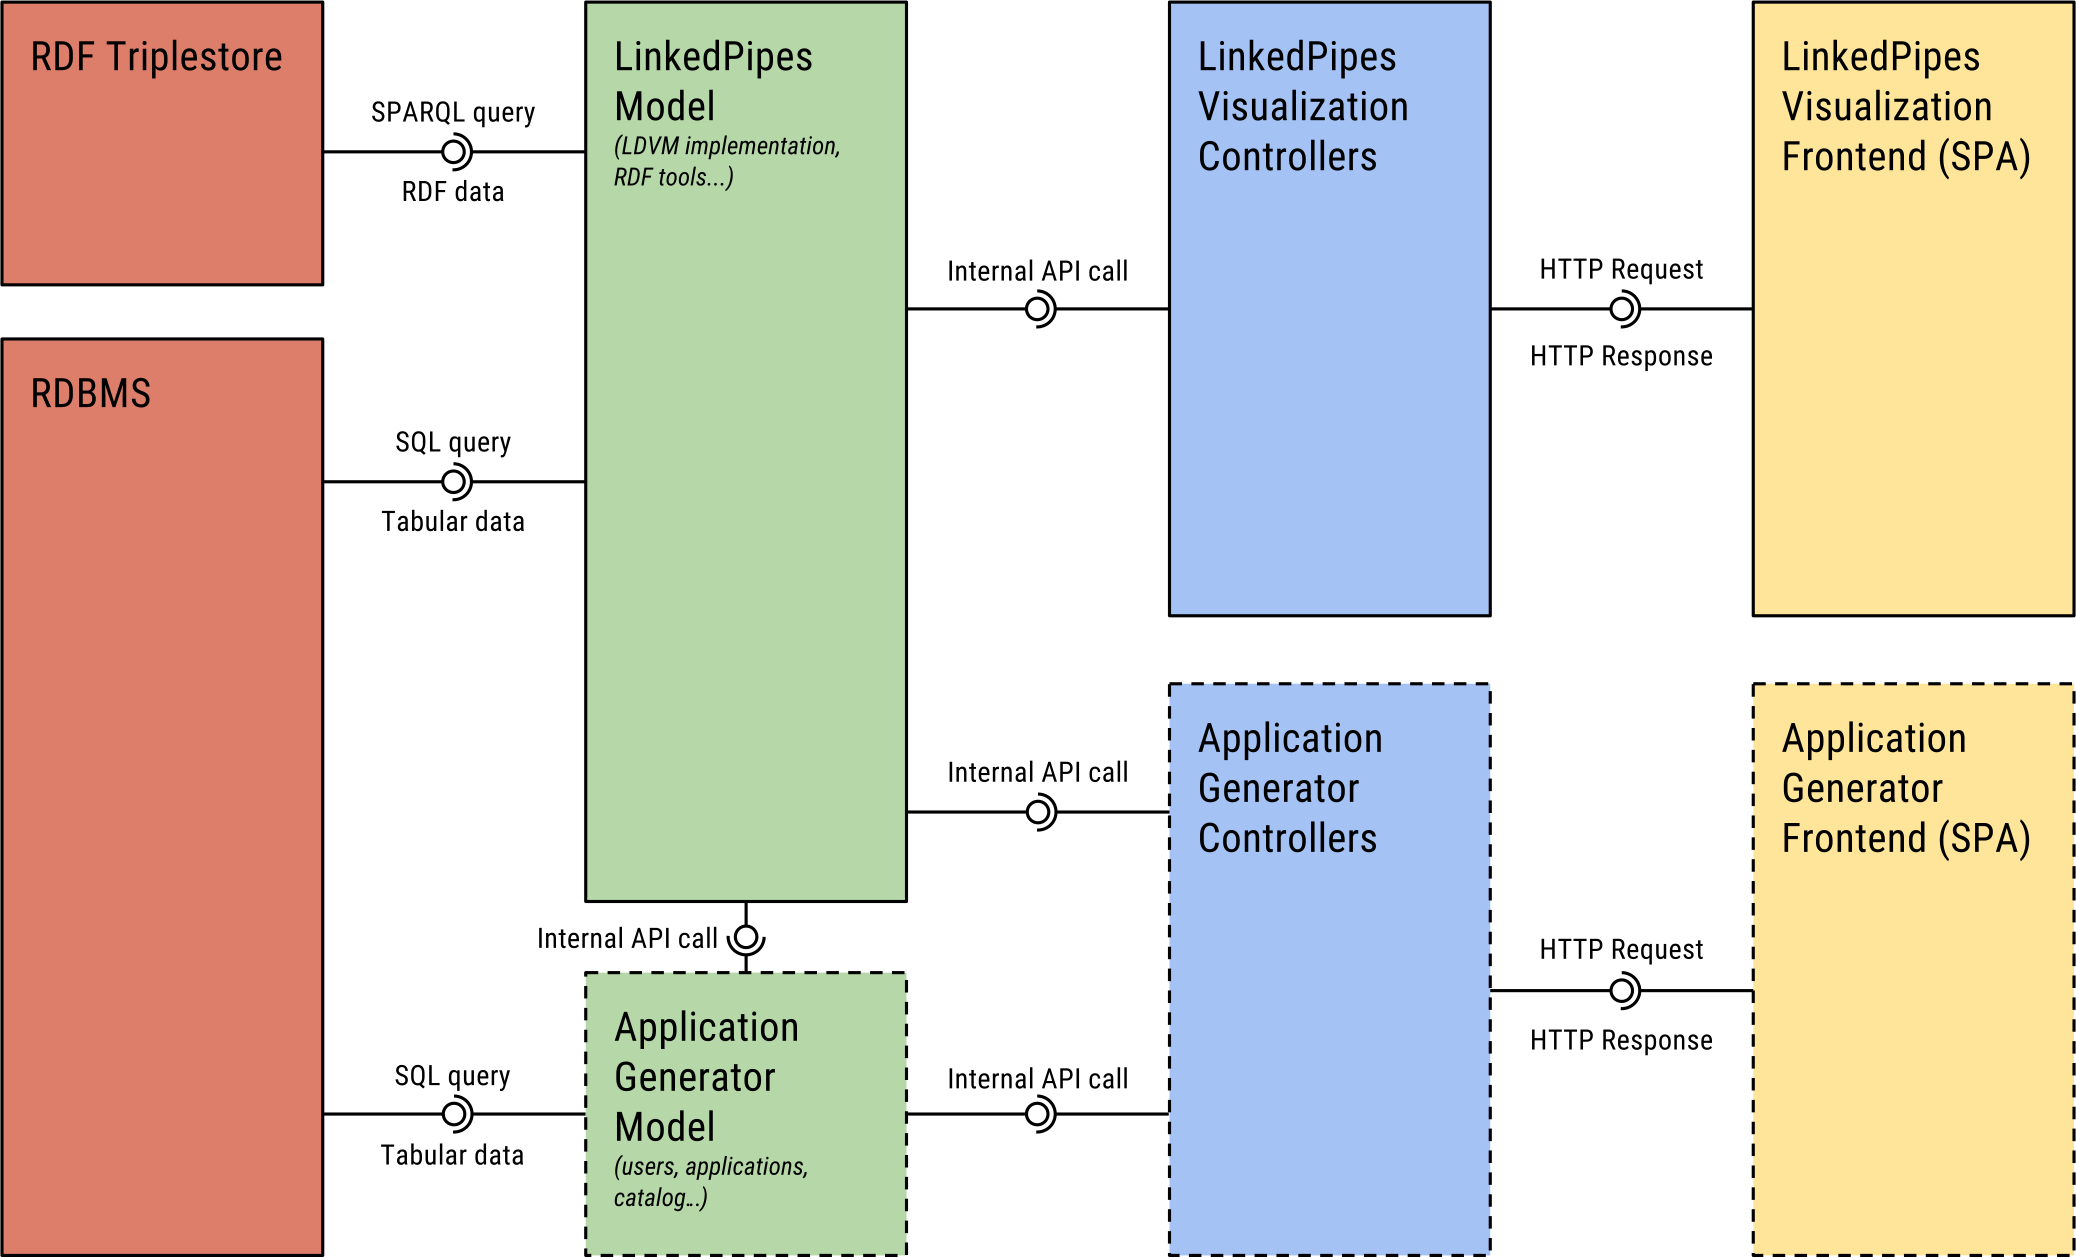
\includegraphics[width=140mm]{img/04_application_generator_architecture.png}
	\caption{Architecture of the \emph{application generator}. Blocks with solid borders are part of the original LinkedPipes Visualization, blocks with dashed borders are newly implemented parts of the \emph{application generator}. The backend follows the standard MVC architecture.} 
	\label{fig:proposed-application-generator-architecture}
\end{figure}

Coming to this realization, we decided to take the path of least resistance and integrate our \emph{application generator} directly into the LinkedPipes Visualization codebase, just as the fist approach suggests. As the result, we could immediately start utilizing the existing patterns and tools for working with RDF. 

Nevertheless, even though both tools live in the same code base, we made sure to keep them as separated as possible. So if we decided in the future to separate both tools or for example replace the underlying LDVM implementation, it should be rather straightforward. How this is achieved can be seen on Figure \ref{fig:proposed-application-generator-architecture}. We will walk through the individual layers of integration in the following subsections.

An important consequence of this unification is that the LDVM implementation instance is shared among the \emph{application generator} and LinkedPipes Visualization. That means that they both use the same set of registered LDVM \emph{components}. We benefit from this as well to an extent as we can utilize existing implemented user interfaces handling some of the LDVM related tasks (e.g. new LDVM \emph{components} are registered to the \emph{generator} through the LinkedPipes Visualization user interface).

\subsection{Frontend}

In LinkedPipes Visualization, the frontend is an SPA living in the client web browser. Its responsibility is to render the user interface which communicates with the backend using the public remote API via HTTP. The frontend part does involve some more complex logic, e.g. necessary for rendering the visualizations themselves, but in general all core business logic (anything related to RDF, the \emph{discovery}, any data transformation or filtering) is almost exclusively dealt with in the backend and the frontend merely serves as the way to communicate with the user. The \emph{application generator} frontend follows this approach as well.

There was an option to re-use the original frontend and just extend it with the functionality that we needed. It already contained some work that we could at first glance use (for example frontend parts of existing \emph{visualizer} plugins, i.e., the actual visualizations). Unfortunately, couple of problems prevented us from doing so. 

\begin{enumerate}
\item The frontend was created just to showcase the capabilities of the underlying LVDM implementation. For this reason, the overall code quality was not  a number one priority. The code was not structured well enough so that we could start extending it. In general, it would take us lots of time to get familiar with it. 
\item The code was not written with certain features (like for example user support or the aforementioned general extendability) in mind.
\item Our \emph{visualizers} (with the separated \emph{configurator} and \emph{application} interfaces) work very differently compared to the \emph{visualizers} of LinkedPipes Visualization.

\end{enumerate}
Having these three reasons in mind, we came to the conclusion that we would have to rewrite a major portion of the original code anyway and therefore we decided to start from the scratch. As a result, there are two existing user interfaces that live within the same application next to each other, available from two different starting URLs.

The frontend itself can be viewed as a standalone application that has its own inner architecture. It is responsible for rendering the user interface which involves many not so simple tasks, including transitions between individual screen, processing user input, processing backend responses (including the the failed ones) and of course visualizations themselves. The architecture is also important because it defines the way the frontend can be extended with new \emph{visualizers}. 

We cannot give any more details about how the frontend is structured as we used a rather uncommon (or perhaps new) development stack with a rather uncommon architecture. We will provide all the necessary knowledge and explanation in the implementation chapter.

\subsection{Backend}

The backend of LinkedPipes Visualization is a standard MVC application, consisting of a \emph{Model} layer, containing various repositories and services that handle the business logic, and \emph{Controllers}, defining the public remote API. The integration of our \emph{application generator} into LinkedPipes Visualization is a matter of adding new controllers, repositories and services to the codebase that will cover the new functionality (Figure~\ref{fig:proposed-application-generator-architecture}).

The vast majority of controllers in both LinkedPipes Visualization and the \emph{application generator} handle the asynchronous HTTP requests coming from the frontend. The role of a controller in this typical case is just to translate the HTTP request into an API call to the \emph{Model} layer and send the response back. All controllers together define a public remote API interface.

Even though we could re-use some of the API methods available from the LinkedPipes Visualization controllers (e.g. those for controlling the \emph{discovery} algorithm), we decided not to do that to avoid hidden dependencies between the frontend and the backend. Dependencies within the  codebase (for example between the \emph{Controller} layer and the \emph{Model} layer) are easy to discover using a static program analysis. Simply put, the whole backend is one piece of code and so if there is a broken dependency, the code will not compile. That is not true for the remote API. Therefore the \emph{application generator} frontend strictly uses only those remote API methods that are handled by the \emph{application generator} controllers (as seen on Figure \ref{fig:proposed-application-generator-architecture}). 

The \emph{Model} layer consists of various repositories and services that handle the business logic. Each repository (or a service) covers a limited area of functionality and exposes a clearly defined public API. Whereas repositories usually work on a lower level, providing for example basic access to RDBMS, services involve a higher level logic.

The new services and repositories that are part of the \emph{application generator} are either completely independent (e.g. service handling the users) or create a one-way dependency on some of the existing repositories or services from LinkedPipes Visualization (this can also be seen on Figure \ref{fig:proposed-application-generator-architecture}). For example, there is a \texttt{PipelineDiscoveryRepository} in the original LinkedPipes Visualization codebase that can return a list of executed LDVM \emph{discoveries}. This repository is, however, completely unaware of users. So we implemented our own custom service, \texttt{DiscoveriesService}, that utilizes the aforementioned repository and adds all the extra functionality related to users (e.g. it can return list of executed \emph{discoveries} by a given user).

Figure \ref{fig:proposed-application-generator-architecture} might suggest that our extension of the \emph{Model} layer directly communicates with RDBMS. Strictly speaking, that is not true because we are utilizing some low level services to access the database and those services could still be considered part of the \emph{Model} layer.

\subsection{Separation from LinkedPipes Visualization}

What is important is that all \emph{application generator} related functionality, even though within the same codebase, is kept separated. The frontend communicates only with our controllers. The backend extension is in a form of a compact layer over the original codebase, consisting of custom controllers, services and repositories. The dependencies on the original codebase, as shown on Figure~\ref{fig:proposed-application-generator-architecture}, are always in a form of utilizing the internal API of LinkedPipes Visualization. It is easy to draw the line where LinkedPipes Visualization ends and our \emph{application generator} begins. Only in rare cases, we re-use some low-level utilities from the original codebase.

\subsection{Extendability by new visualizers}

Let us now talk about one distinct feature that the software architecture needs to count with: extendability. In this case, it specifically means the ability to be extended with new \emph{visualizers}. As we have described, a \emph{visualizer} (Subsection \ref{sec:linkedpipes:visualizers}) consists of an RDF definition of the LDVM \emph{component} and a \emph{plugin}. The RDF definition needs to be simply imported to the LDVM instance so that the \emph{discovery} algorithm can start using it. The situation is more complicated with the \emph{plugin} as it needs to be properly integrated both in the backend and in the frontend. How this is done can be seen on Figure \ref{fig:sample-visualizer-structure}.

\begin{figure}
	\centering
	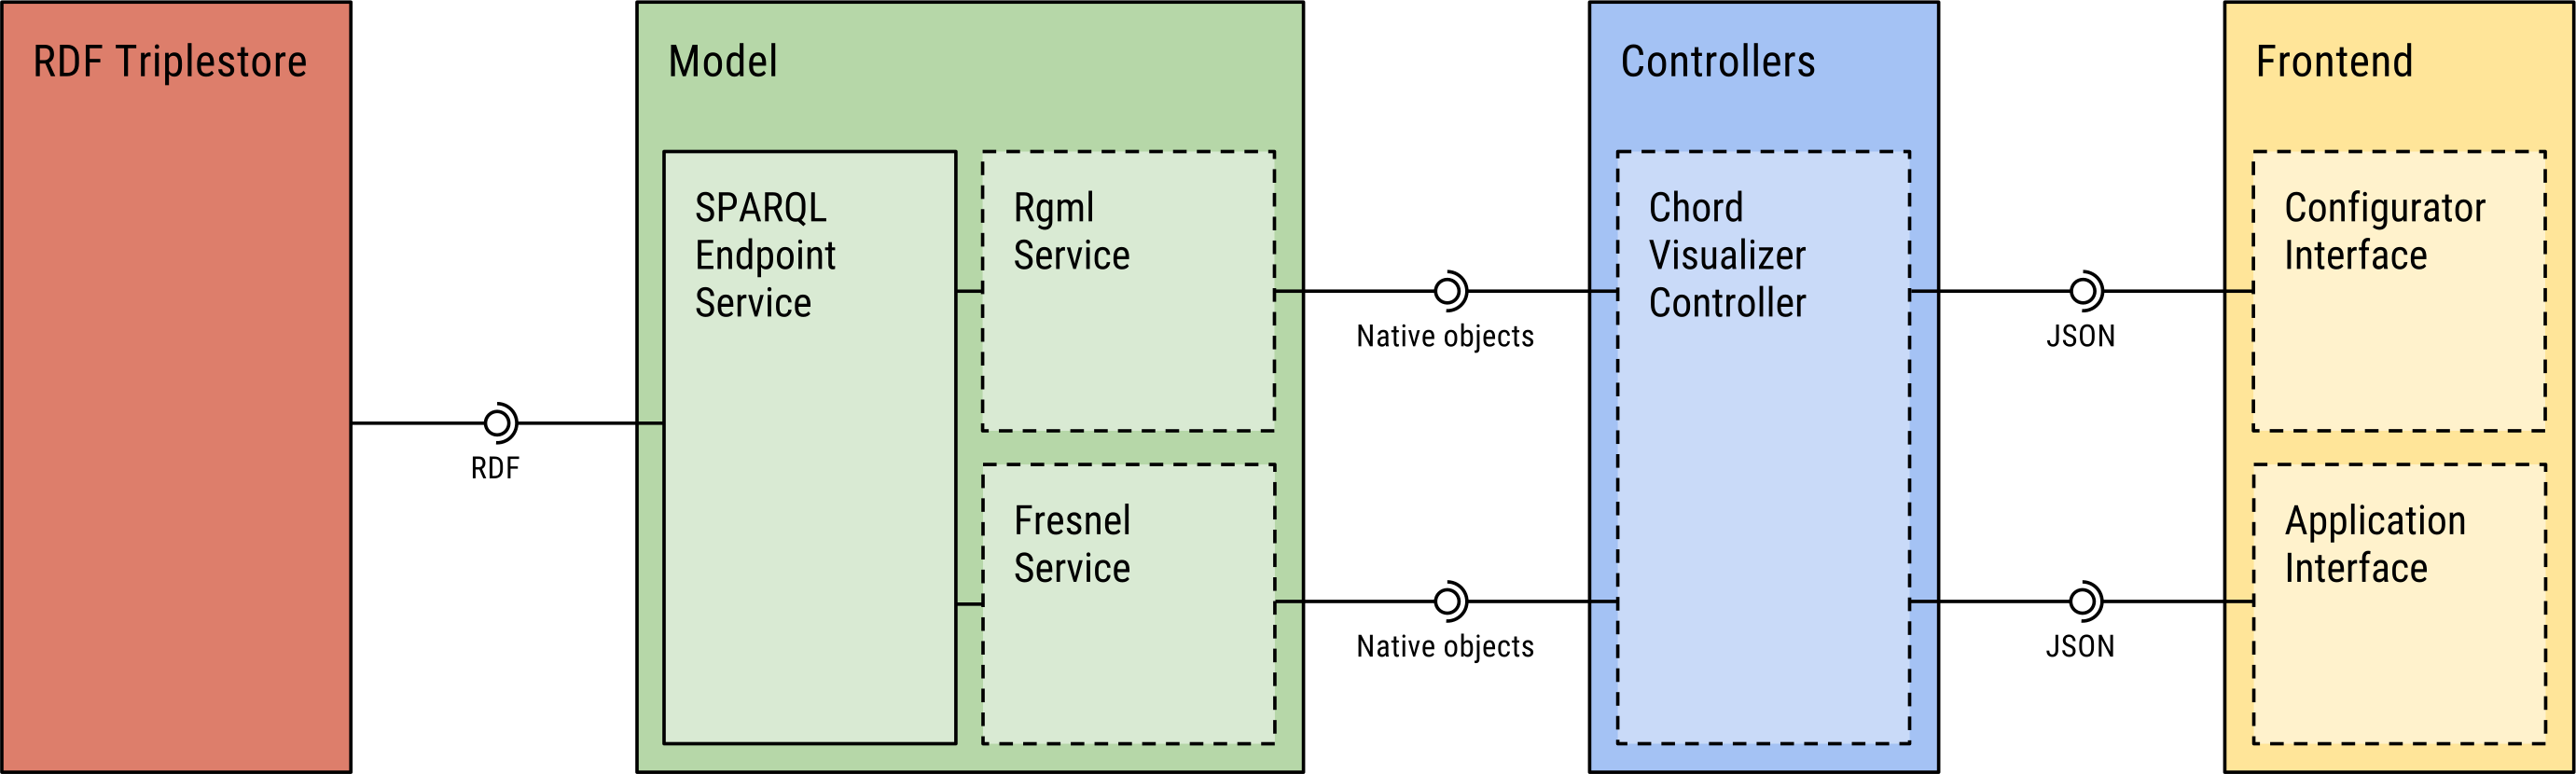
\includegraphics[width=140mm]{img/04_chord_visualizer_structure.png}
	\caption{Architecture of a sample \emph{visualizer}, D3.js Chord Visualizer, showing how it is integrated into the \emph{application generator}. The blocks with dashed borders represent newly implemented components. The label underneath each connections suggests the data format of that particular API.} 
	\label{fig:sample-visualizer-structure}
\end{figure}

The backend part is typically responsible for converting the data from RDF to a format suitable for the visualizer frontend. This functionality is exposed via a remote API that the frontend can utilize. What is important is that individual API methods are rather independent. As long as we keep some kind of system in the API method URLs to avoid conflicts (e.g. define a unique URL prefix for each \emph{visualizer}), we can almost indefinitely extend the API with new methods by adding new controllers and extending the old ones. Obviously, the actual business logic is handled in the \emph{Model} layer but that can be extended in similar manner with new repositories and services.

As we are specifically talking about the backed part of a new \emph{visualizer}, this extension would typically involve a new service adding support for a new RDF vocabulary.  Such a service would have a fairly simple structure as it would most likely just expose methods that take input RDF data as an argument and return the data represented in native domain objects (that will be eventually converted to JSON and sent to the frontend). Given this structure, we can easily add as many similar services to support as many vocabularies as we need without worrying about any conflicts. The extendability is rather straightforward.

On the other hand, each such service would heavily depend on the internal RDF infrastructure of LinkedPipes Visualization. This infrastructure not only provides among other things services to access the triplestore but also defines various conventions for example for how a SPARQL should be expressed in the native code. This is the only case when our code significantly overlaps with the original LinkedPipes Visualization code.

The frontend part contains the \emph{configurator} and \emph{application} interfaces. They both need to be integrated into the rest of the frontend which is a rather complex task. Firstly, there must be a mechanism that based on the application type (i.e., the LDVM \emph{visualizer} component) dynamically selects the correct \emph{configurator} (or \emph{application}) interface and shows it to the user. Secondly, not only does the (let us say) \emph{configurator} interface have to be able to communicate with the rest of the frontend, but it also should  look like it is a part of it, i.e., it should fit in and follow the recommended visual design guidelines. Therefore the integration in this case is significantly more complicated than adding a new independent service to the \emph{Model} layer.

Unfortunately, the integration process heavily depends on the custom chosen development stack that we used for the frontend. Without explaining the basic principles of how the frontend is structured, we are not able to provide any general information about how this works. This, including the internal frontend API, will be properly explained in the next implementation chapter.

\subsection{Steps to implement a new visualizer}

Let us summarize the previous subsection by simply listing the base tasks necessary to integrate a new \emph{visualizer} to the \emph{application generator}. Note that the tasks are not numbered. Clearly, one has to start with defining the RDF data format (i.e., how the input data for the \emph{visualizer} should look like) and with designing the API. Once this is done, the order in which the following tasks are carried out is irrelevant.

\begin{itemize}
\item Define and add the LDVM \emph{visualizer} component so that the \emph{discovery} algorithm can use it.
\item Implement necessary services in the \emph{Model} layer that extract RDF data in custom vocabularies and convert them to native objects.
\item Implement the \emph{visualizer} controller that utilizes the services and exposes their functionality via a public remote API.
\item Implement the \emph{configurator} and \emph{application} user interfaces and integrate them into the frontend. 
\end{itemize}

\subsection{API design}

The whole application consists of separate layers (Figure \ref{fig:proposed-application-generator-architecture}). On the top level the application is split into the frontend and the backend. The backend is then organized into layers as well, according to the MVC architecture. Finally, the \emph{Model} layer typically consists of multiple levels of abstraction for each problem it covers (repositories, services etc). Each layer defines a public API using which it can be utilized by higher layers.

Let us talk for now about the public remote HTTP API that is exposed by the backend, i.e., the API that is used for the communication between the frontend and the backend. The API consists of many smaller APIs that each covers a limited area of functionality and is represented by a single controller. All the controllers together cover everything that is required by the frontend, i.e., the complete functionality of the \emph{application generator} (remember that on this level, we are not utilizing anything from the original API of LinkedPipes Visualization at all). Let us now walk through the base individual APIs which will give the reader an idea of what the \emph{application generator} do and how it works.

\begin{itemize}
\item \textbf{Application API} -- returns a generated application and its configuration.
\item \textbf{Authentication API} -- authentication and registration of users.
\item \textbf{Catalog API} -- browsing through the catalog of published applications.
\item \textbf{Common Visualizer API} -- common functionality for all visualizers (e.g. dereferencing labels).
\item \textbf{Create Application API} -- the process of creating an application which includes browsing data sources, running the \emph{discovery}, executing selected \emph{pipelines}.
\item \textbf{Dashboard API} -- browsing and basic management of the user content, which includes applications, data sources and \emph{discoveries}.
\item \textbf{Manage Application API} -- updating, deleting and configuring a generated application.
\todo[color=green!40]{Jednotlivá API zjevně ve většině případů odpovídají jednotlivým obrazovkám uživatelského rozhraní. Vzniklo to organanicky, prostě jak jsem experimentoval a postupně vyvíjel frontend, tak jsem si tímto způsobem dopisoval backendové API a úplně nad tím nepřemýšlel. Je mi jasné, že ze SWI hlediska není ideální vázat API tímto způsobem na uživatelské rozhraní. Reálně nicméně je ten backend dost jednoduchý a v podstatě tam k problémům, konkrétně duplikaci funkcionality pro různé obrazovky, nedochází, resp. každá ta obrazovka má stejně ty požadavky trochu jiné, takže jsem definoval API metody na míru tomu, co jsem potřeboval. Roli hrálo i to, že v některých případech je nutné, aby byl přihlášen uživatel, což se právě typicky lišilo obrazovka od obrazovky, a authorizaci mám vyřešenou na úrovni celého controlleru, tj. jakýsi návrhový záměr tam je. Mám to nějak řešit, tj. ještě přepsat kód, nebo udělat v textu nějakou poznámku, že jsem si toho vědom, nebo to můžu prostě nechat být?}
\end{itemize}

These APIs cover the general agenda of the \emph{application generator}. Then each \emph{visualizer} defines its own API (its own controller, see Figure \ref{fig:sample-visualizer-structure}) that covers only the functionality of this particular \emph{visualizer} (note that this is rather a convention). Also note that some of the APIs are completely public (e.g the \textbf{Catalog API}), most of them, however, require the user to be authenticated.

Let us now  have a look at a short scenario showing how the API works. In this scenario, the user will initiate the LDVM \emph{discovery} algorithm and then watch the progress on the screen.

In the preceding step, the user selected the data sources he is interested in. Now he clicks the "Run Discovery" button to initialize the \emph{discovery}. The whole process can be seen on Figure \ref{fig:api-run-discovery-diagram}. The frontend makes an asynchronous HTTP request to the backend. The request is first processed on the \emph{Controller} layer which, among other things, verifies that the user is properly authenticated. The request is then passed on to the \emph{Model} layer where the \texttt{Pipeline Service} starts the actual \emph{discovery} of selected data sources. The \emph{discovery} might take some time so the request does not wait for it to finish. The \texttt{Pipeline Service} simply returns an ID assigned to this particular \emph{discovery}. This ID is what is finally delivered back to the frontend.

\begin{figure}
	\centering
	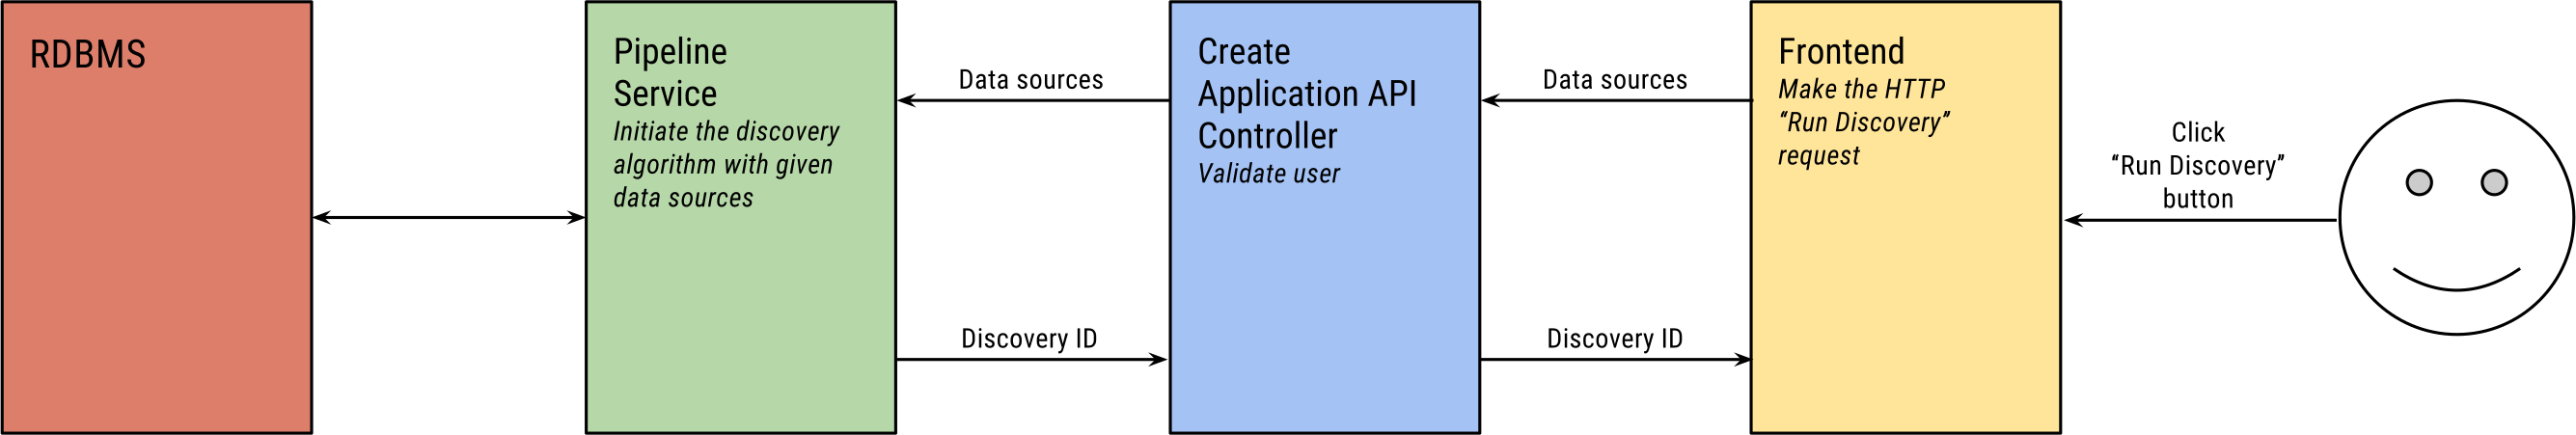
\includegraphics[width=140mm]{img/04_api_run_discovery_diagram.png}
	\caption{Diagram showing the process of running the \emph{discovery} algorithm from the API perspective. The face represents the user initiating the request.} 
	\label{fig:api-run-discovery-diagram}
\end{figure}

As the \emph{discovery} continues, it updates its current status in RDBMS. It also stores to RDBMS the \emph{pipelines} that has been discovered so far. The frontend uses the acquired \emph{discovery} ID to periodically poll the backend for this information until the \emph{discovery} finishes. This way the user can see online on the screen the current status of the \emph{discovery} and also the discovered \emph{pipelines}. This request can be seen on Figure \ref{fig:api-get-discovery-diagram}.

In LinkedPipes Visualization, this particular part is implemented differently. Instead of periodical polling, the \emph{discovery} algorithm output flows through a WebSocket \footnote{\url{https://tools.ietf.org/html/rfc6455}} which is opened between the frontend and the backend. In many ways this solution is more elegant. Only one connection has to be maintained and the updates are pushed to the frontend almost instantly. Unfortunately, in the current implementation in LinkedPipes Visualization, once a WebSocket to a particular \emph{discovery} is closed (e.g. because the user closes the page), it cannot be re-opened again. That means that the user loses the option to watch the \emph{discovery} algorithm progress online. In this sense, our implementation is better as it allows the user to leave and come back anytime later. If the \emph{discovery} has not finished yet, the polling is automatically restored.
\begin{figure}
	\centering
	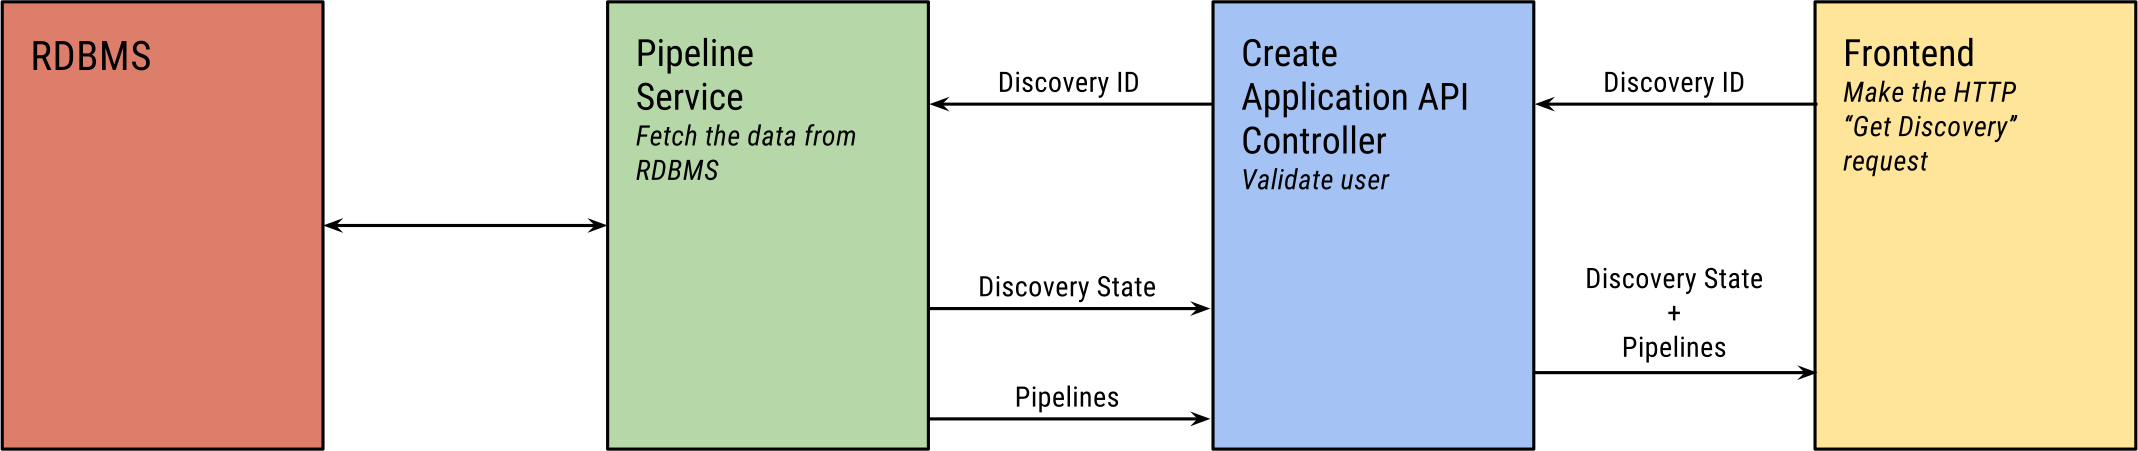
\includegraphics[width=140mm]{img/04_api_get_discovery_diagram.png}
	\caption{Diagram showing the process of fetching the \emph{discovery} algorithm status and the discovered pipelines from the API perspective.} 
	\label{fig:api-get-discovery-diagram}
\end{figure}






\chapter{Implementation}

In this chapter, we will go through our \emph{application generator}, explaining in detail how it works and how it is implemented from the inside. We will focus both on the \emph{platform} aspect and the \emph{framework} aspect. As for the \emph{platform} aspect, we will show how a non-developer can use the new \emph{platform} to generate and share Linked Data based applications. As for the \emph{framework} aspect, we will provide a potential developer with a step-by-step guide for how to implement a new \emph{visualizer}. As our generator is built on top of LinkedPipes Visualization, its official name is LinkedPipes Application Generator. For brevity, we will refer to it simply as to (our) \emph{application generator}. 

\section{Overview}

Before we dive into technical details, let us walk the reader through the \emph{application generator} features from a user perspective. We will start by describing a sample use case scenario and then we will continue with individual \emph{platform} features.

\subsection{Sample use case scenario}
\label{sec:implementation:use-case-scenario}

In this scenario, we will utilize the D3.js Chord Visualizer and the Asylum Seekers 2015 data set. Both will be properly described later in a separate chapter dedicated to this particular visualizer. Let us say that our fictional user is a journalist writing an article on the refugee crisis. He comes across our \emph{application generator} and finds there the Asylum Seekers 2015 data set. The Figures \ref{fig:scenario-01-browse-data-sources} to \ref{fig:scenario-11-embedded-application} show step-by-step how the journalist can use our tool to create an interactive application and share it with his readers.

The actual mechanics of this visualizer will be explained later in the aforementioned separate chapter. Nevertheless, on a more general level this scenario nicely illustrates the principles that we suggested in the system proposal (Section \ref{sec:proposal:features}). The selected data set is automatically \emph{analyzed} and an appropriate visualization is offered to the user (Figure \ref{fig:scenario-02-discovery-result}). The configuration phase allows the user to work with the data and to affect the final shape of the application before it gets published. He can select for the visualization only the data he (or his audience) is interested in (Figure \ref{fig:scenario-05-search-graph}). He can even extend the data set itself with missing information (Figure \ref{fig:scenario-08-custom-label-editor}). Finally, the application can be easily shared using its public URL (Figure \ref{fig:scenario-09-published-app}).

What is also clear is that none of these steps require any advanced programming knowledge. The process is very \emph{non-developer friendly}. The only exception in this case is the preparation of the data set. Unfortunately, the original data are not available in RDF and the conversion has to be done by an expert. Nevertheless, once the data set is prepared and available in the \emph{application generator}, it can become a source for a large number of different applications.

\begin{figure}
	\centering
	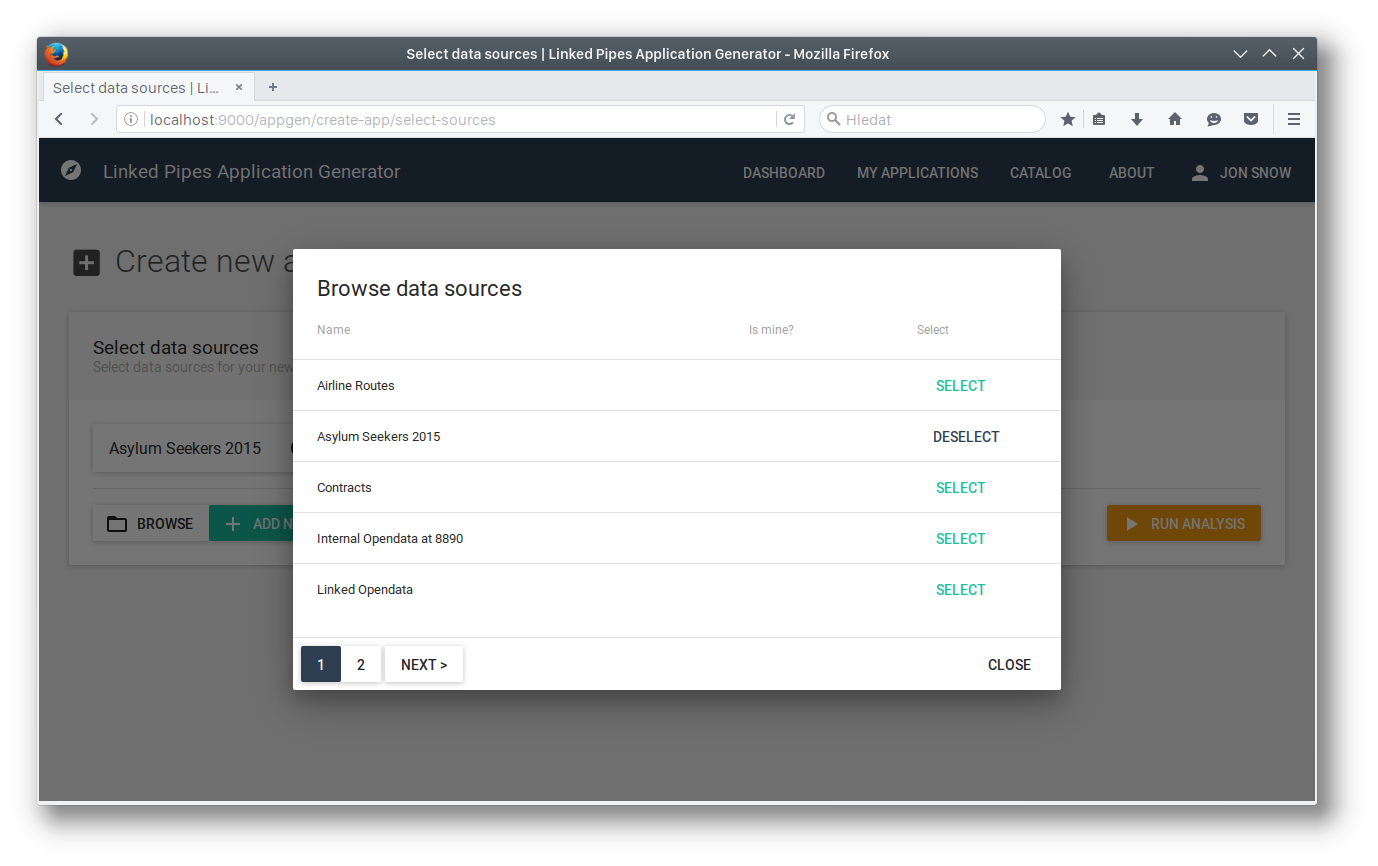
\includegraphics[width=145mm]{img/05_scenario_01_browse_data_sources.png}
	\caption{Use case scenario: Data source browser. The journalist selects the Asylum Seekers 2015 data set.}
	\label{fig:scenario-01-browse-data-sources}
\end{figure}

\begin{figure}
	\centering
	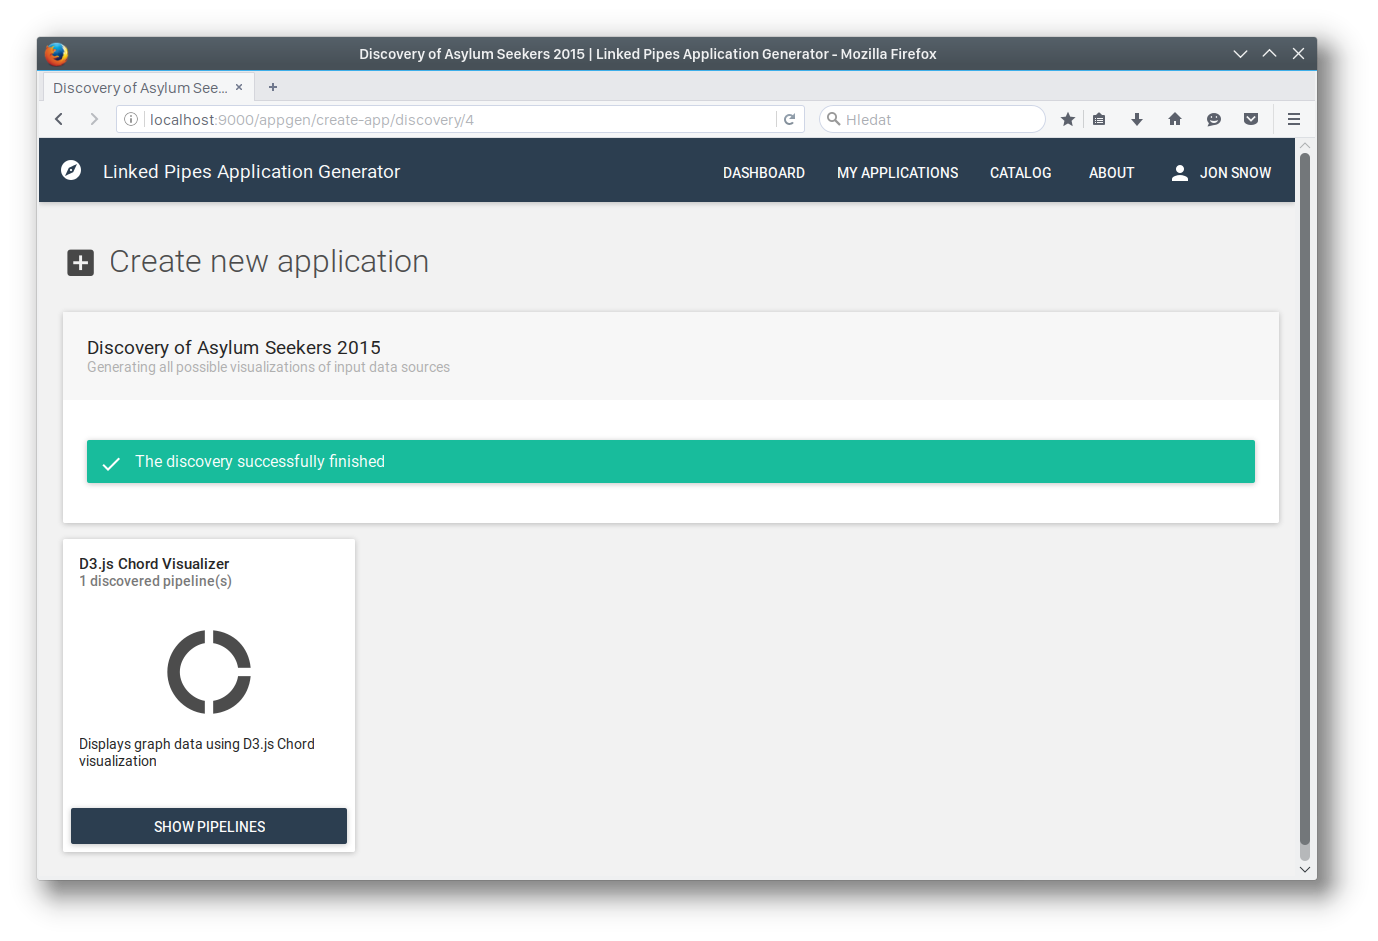
\includegraphics[width=145mm]{img/05_scenario_02_discovery_result.png}
	\caption{Use case scenario: Discovery result. The journalist can see that the Asylum Seekers 2015 data set can be visualized only using the D3.js Chord Visualizer. He runs the one discovered LDVM \emph{pipeline} that ends with this particular LDVM \emph{visualizer component}.}
	\label{fig:scenario-02-discovery-result}
\end{figure}

\begin{figure}
	\centering
	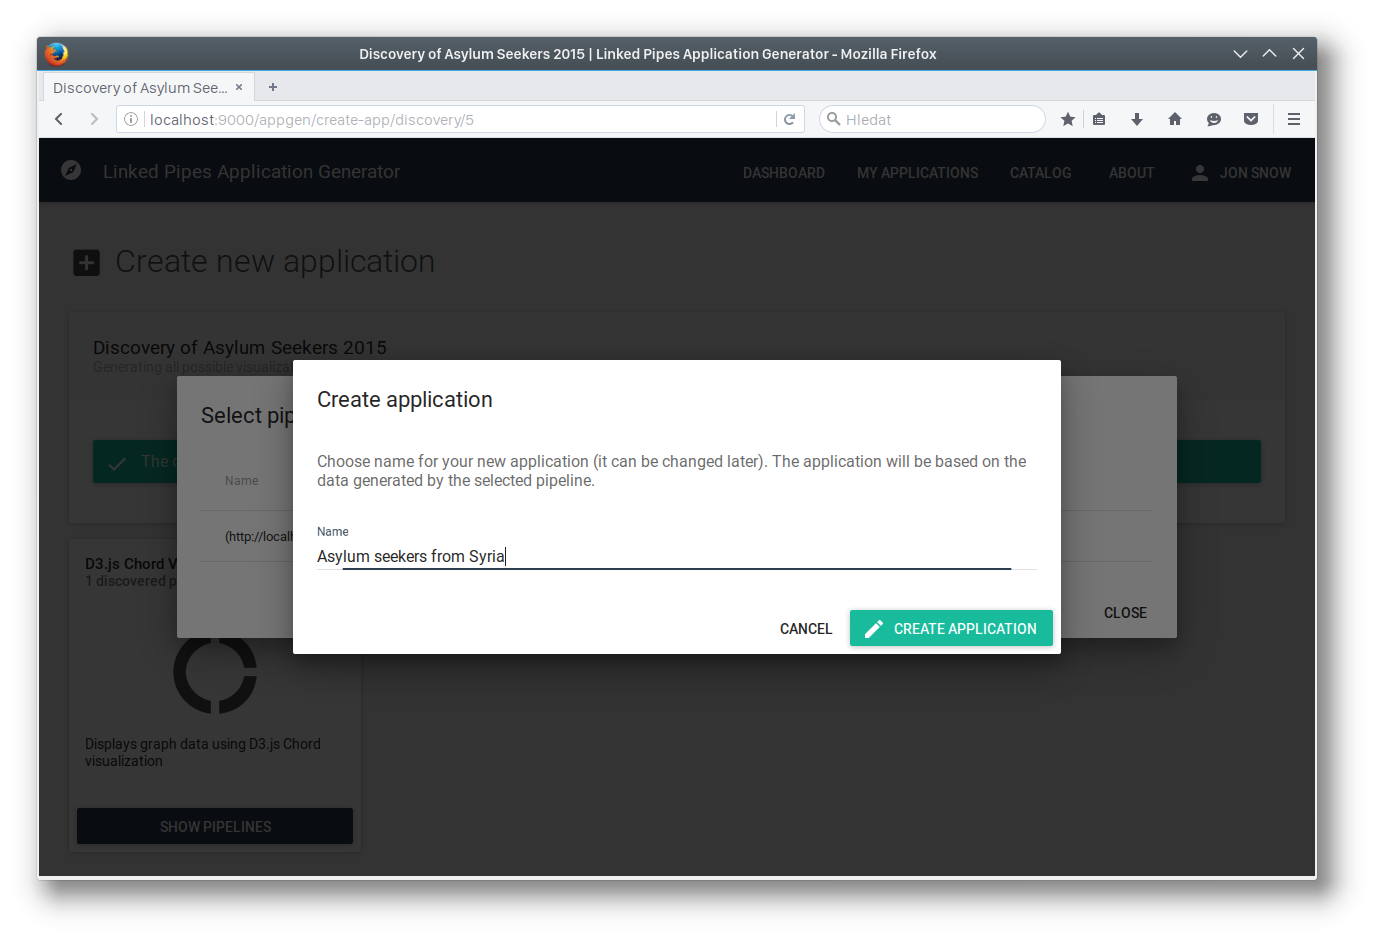
\includegraphics[width=145mm]{img/05_scenario_03_create_application.png}
	\caption{Use case scenario: Create application dialog. When the \emph{pipeline evaluation} is done, the user can proceed by creating an application.}
	\label{fig:scenario-03-create-application}
\end{figure}

\begin{figure}
	\centering
	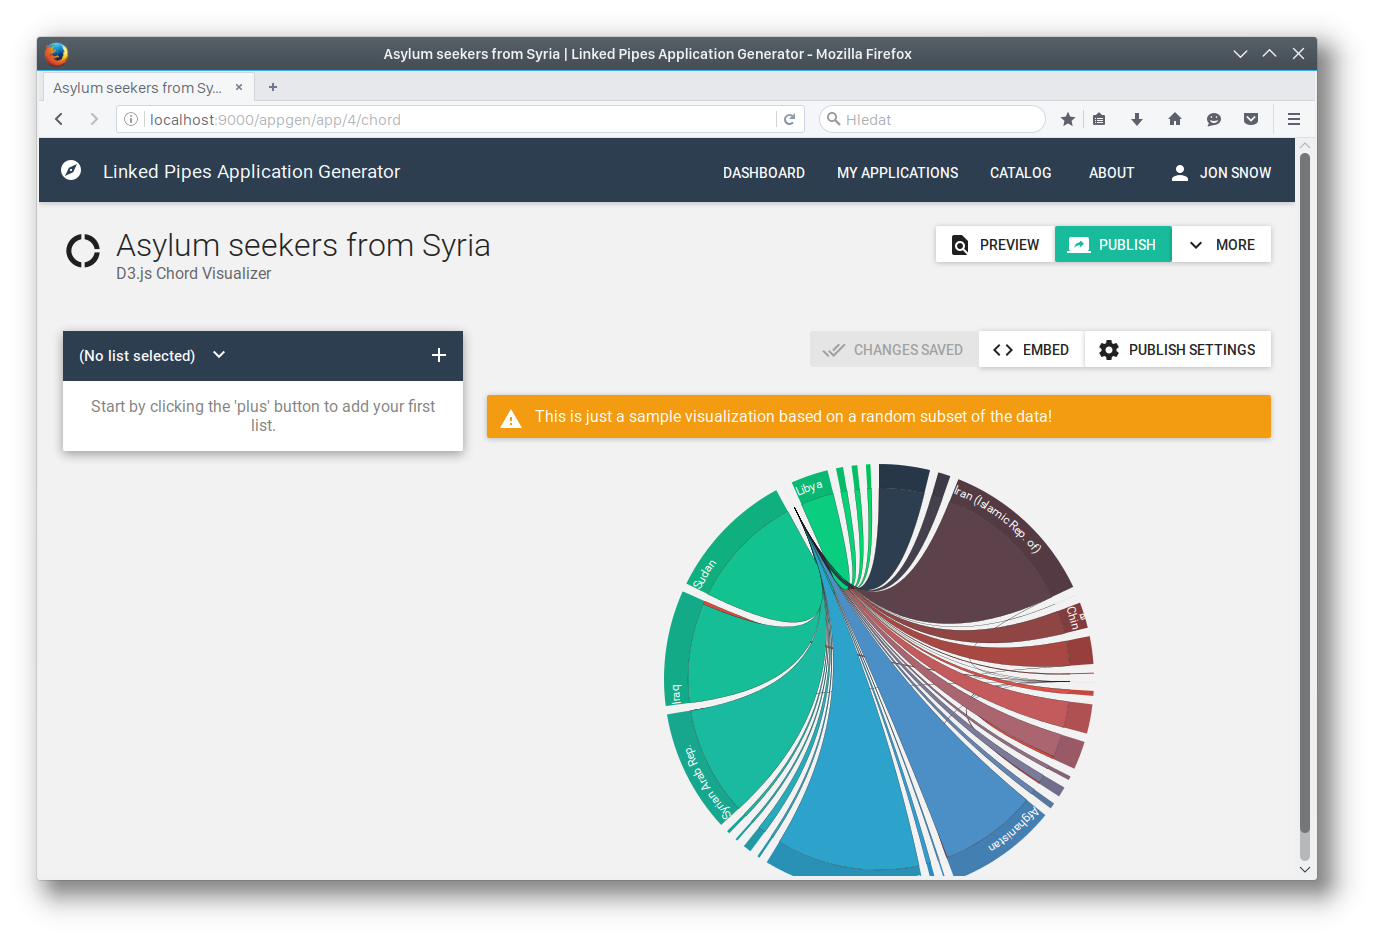
\includegraphics[width=145mm]{img/05_scenario_04_graph_sample.png}
	\caption{Use case scenario: Configurator of D3.js Chord Visualizer. Immediately after the application is created, the journalist is presented with a random sample visualization of the data.}
	\label{fig:scenario-04-graph-sample}
\end{figure}

\begin{figure}
	\centering
	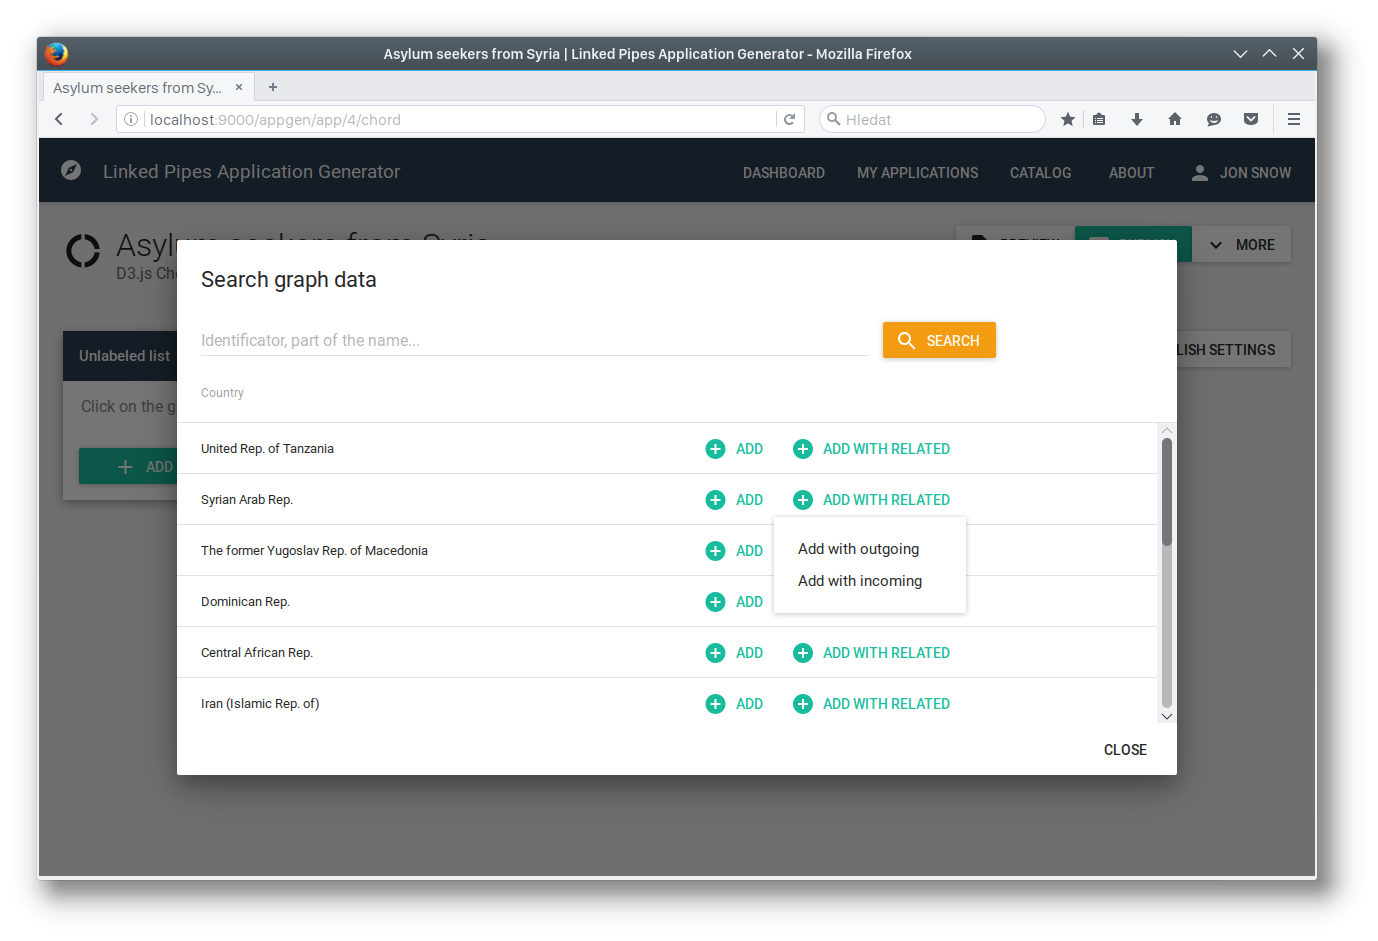
\includegraphics[width=145mm]{img/05_scenario_05_search_graph}
	\caption{Use case scenario: Search dialog. The journalist wants to create a visualization of asylum seekers coming from Syria. He uses the search feature to find Syria in the data set and adds it together with all target countries to the visualization \emph{list}.}
	\label{fig:scenario-05-search-graph}
\end{figure}

\begin{figure}
	\centering
	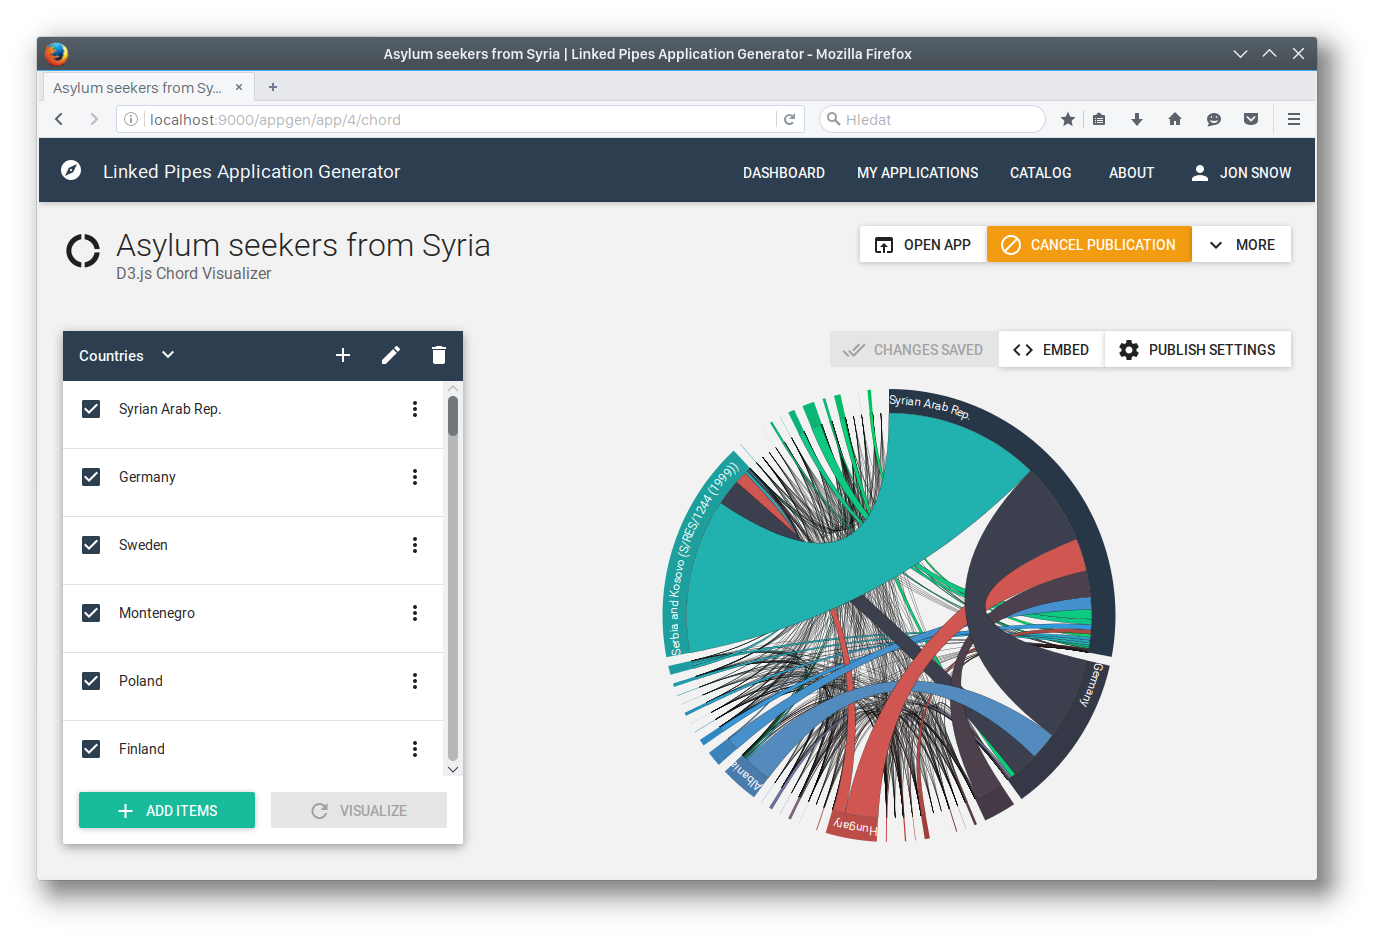
\includegraphics[width=145mm]{img/05_scenario_06_ready_application}
	\caption{Use case scenario: Visualization of selected countries. The journalist is now presented with the chord diagram of the countries he added into the \emph{list}.}
	\label{fig:scenario-06-ready application}
\end{figure}

\begin{figure}
	\centering
	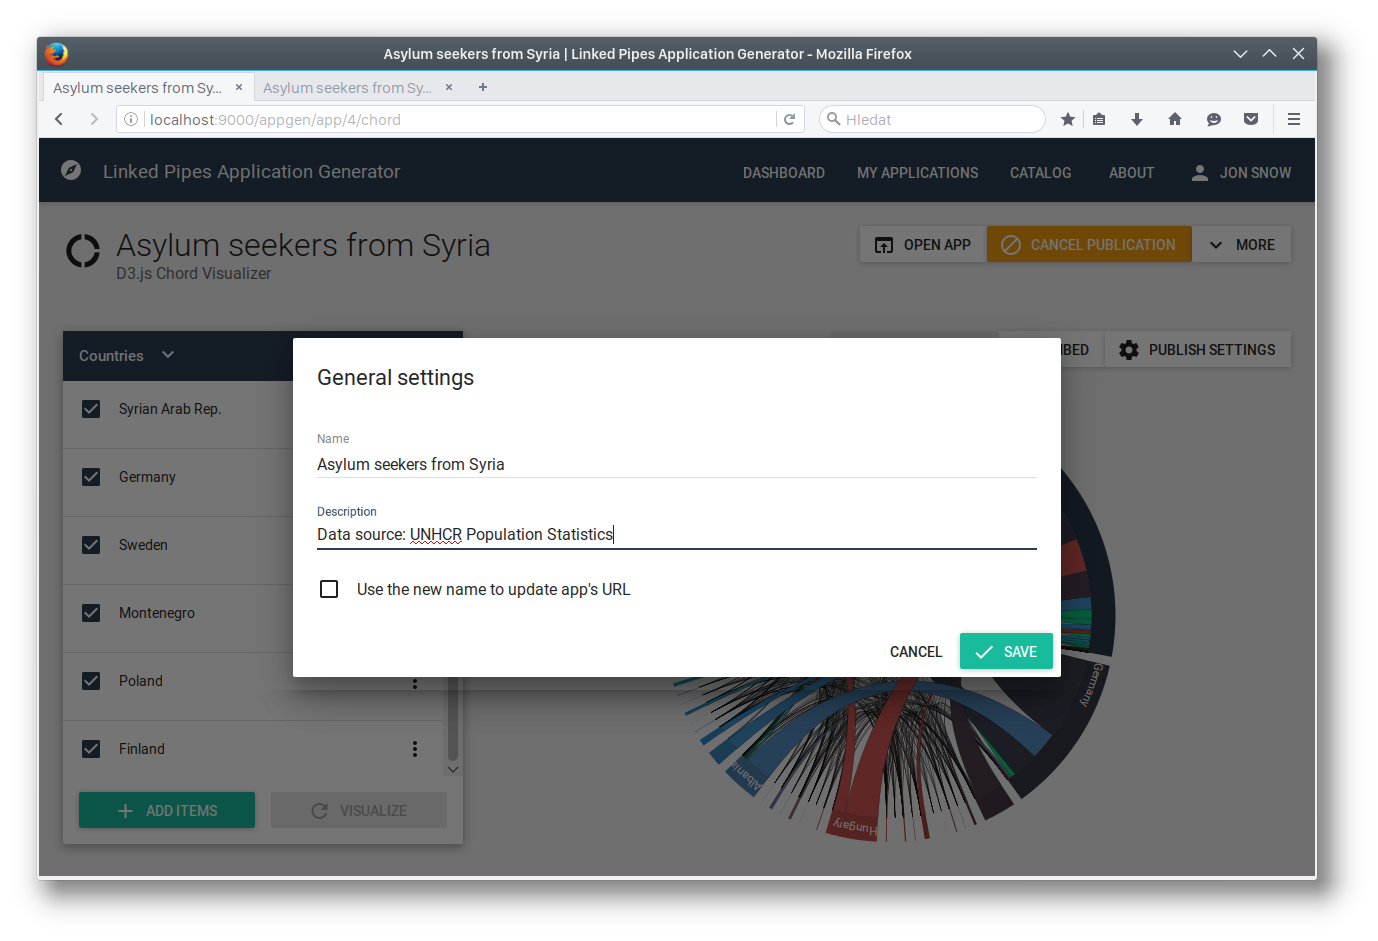
\includegraphics[width=145mm]{img/05_scenario_07_general_settings}
	\caption{Use case scenario: General application settings. The journalist can also provide the application description (in this case he uses it to explicitly mention the source of the data).}
	\label{fig:scenario-07-general-settings}
\end{figure}

\begin{figure}
	\centering
	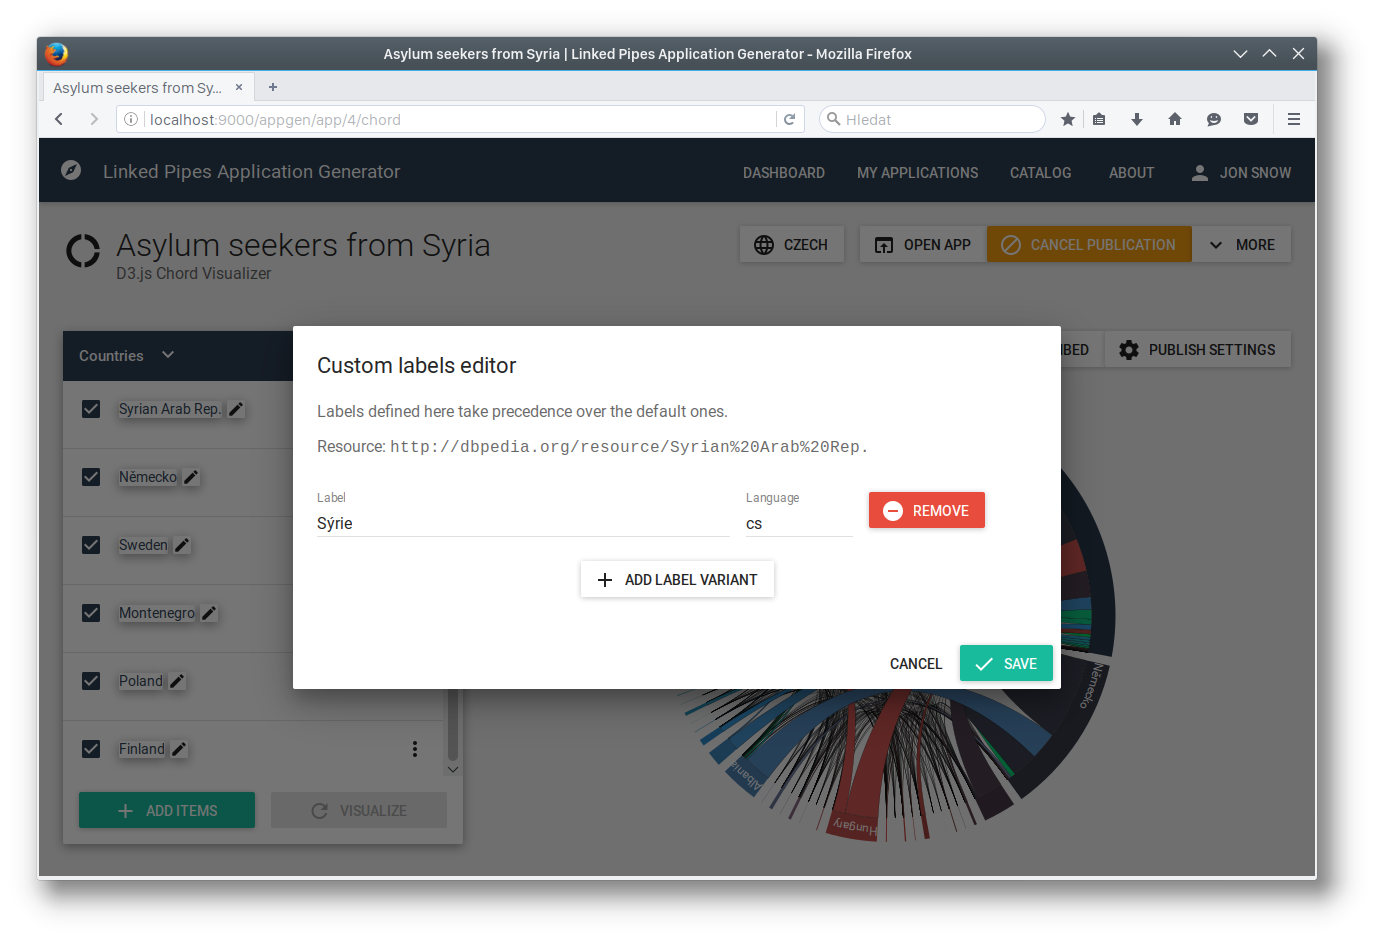
\includegraphics[width=145mm]{img/05_scenario_08_custom_label_editor}
	\caption{Use case scenario: Custom labels editor. The journalist is targeting Czech audience but the country names in the data set are in English. The configurator lets the journalist provide his own names that will override the default ones. }
	\label{fig:scenario-08-custom-label-editor}
\end{figure}

\begin{figure}
	\centering
	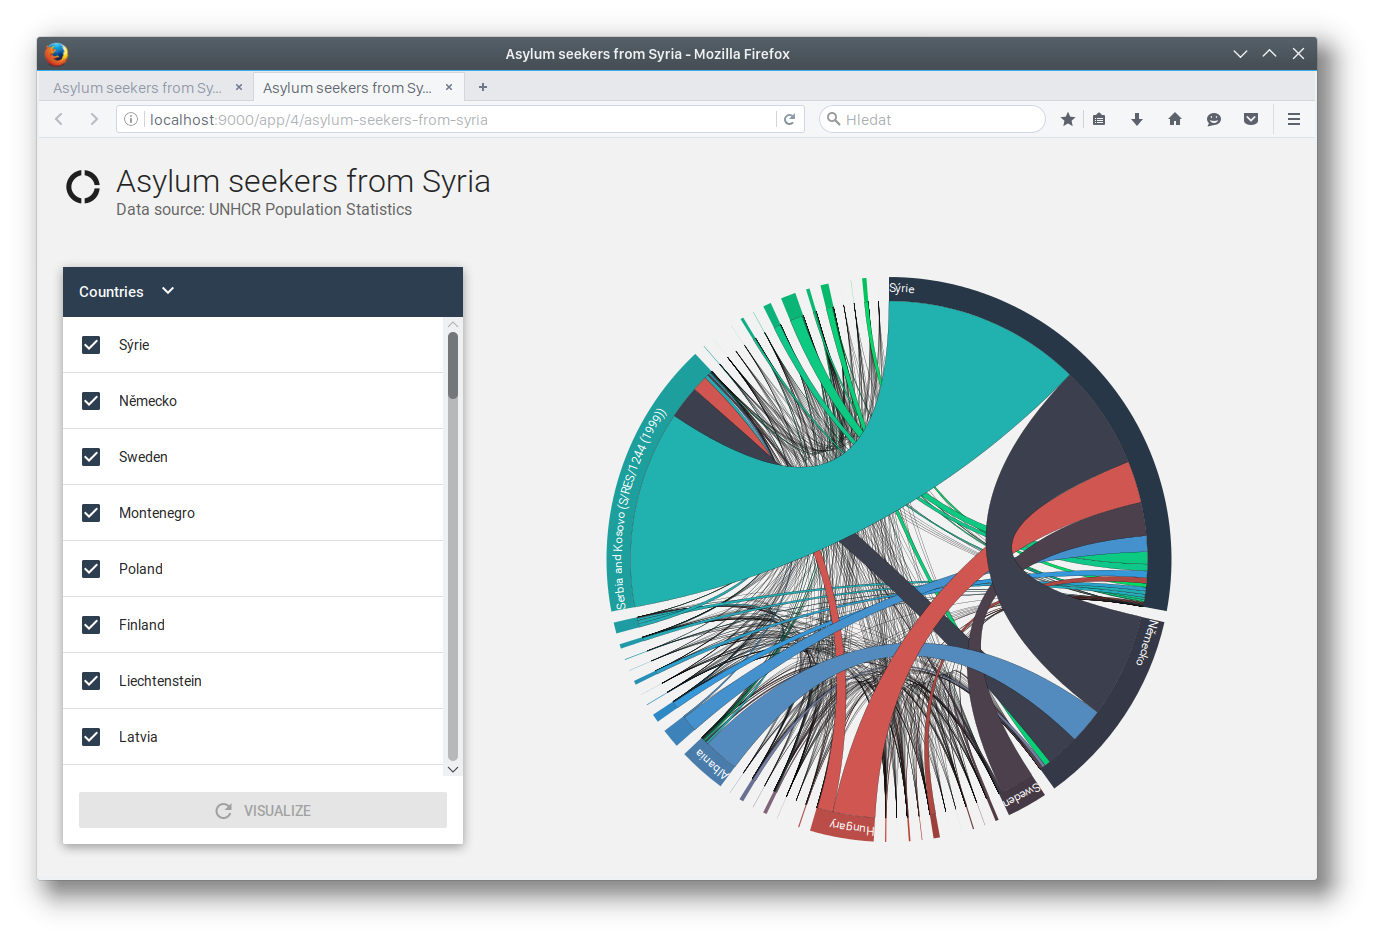
\includegraphics[width=145mm]{img/05_scenario_09_published_app}
	\caption{Use case scenario: Published application. This is what the journalist's readers will see when the application gets published. Using the menu on the side, the users can switch on/off individual countries in the chord diagram.}
    \label{fig:scenario-09-published-app}
\end{figure}

\begin{figure}
	\centering
	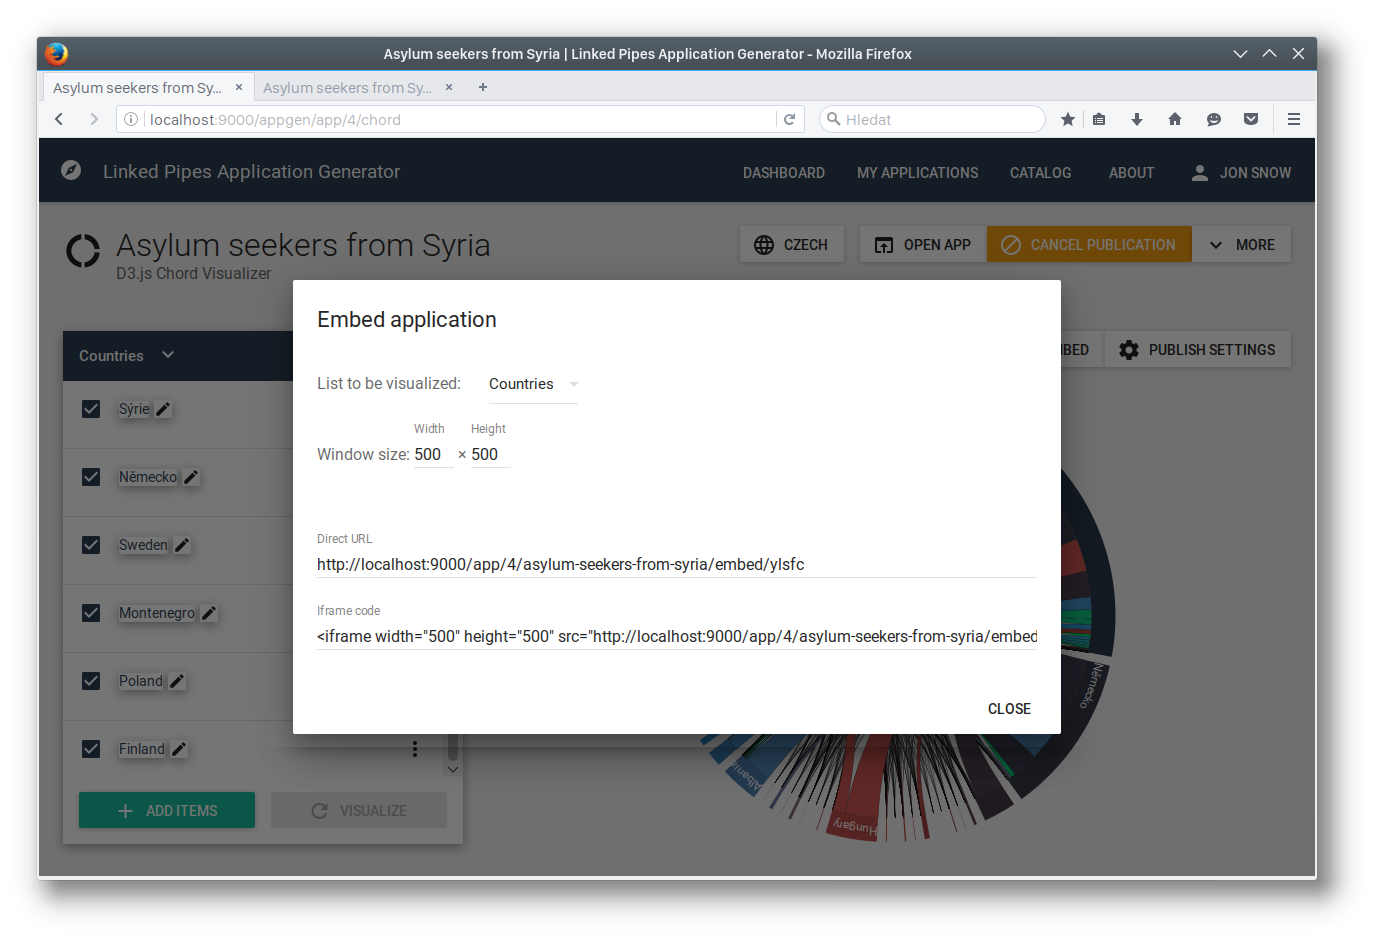
\includegraphics[width=145mm]{img/05_scenario_10_embed_application}
	\caption{Use case scenario: Embed application dialog. The journalist may decide to embed the chord diagram directly into his article.}
    \label{fig:scenario-10-embed-application}
\end{figure}

\begin{figure}
	\centering
	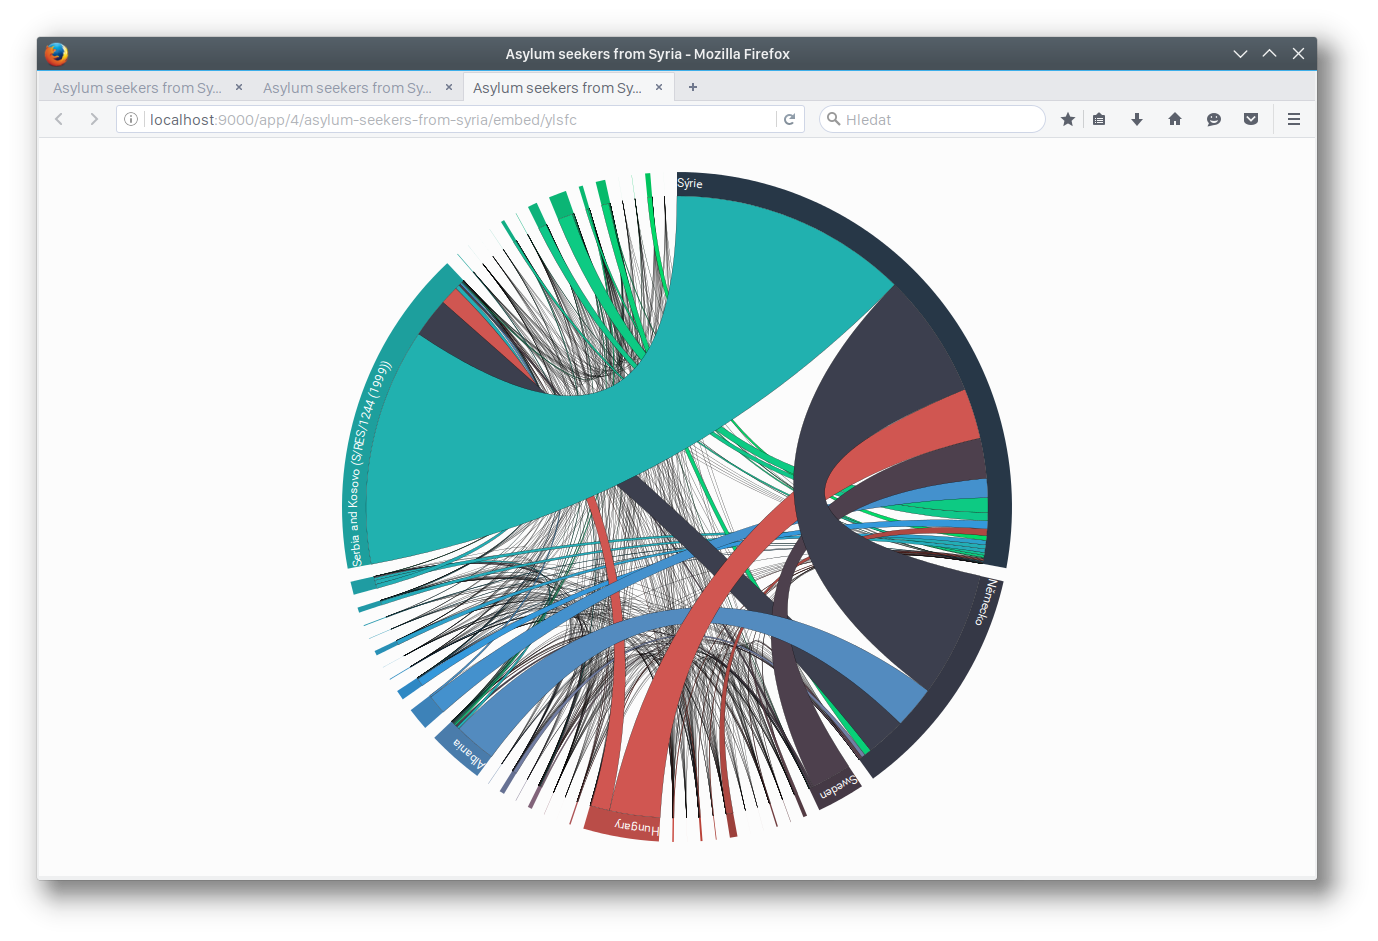
\includegraphics[width=145mm]{img/05_scenario_11_embedded_application}
	\caption{Use case scenario: Embedded application. In this form, stripped from all controls to the bare visualization, it is perfect for direct embedding into web pages.}
    \label{fig:scenario-11-embedded-application}
\end{figure}


\subsection{Users}

Everyone who wants to use our \emph{application generator} needs to create an account first. At this moment, a user can either create a standard local account protected by a password or he can log in with his Google account. No other providers are currently supported. As the user works with the \emph{application generator}, all his applications, data sources and discoveries are linked to his account and no one else can access it. E.g. an application can be configured only by its owner and before it is published, only the owner can view it.

One exception are \emph{administrator} accounts which work similarly to root users known from Unix systems. Such users can access and update any applications, data sources or discoveries in the system. The first user to register in our \emph{application generator} automatically becomes an administrator. The others have to be manually appointed (which is currently not possible through the user interface and has to be done by directly updating the database record).

\begin{figure}
	\centering
	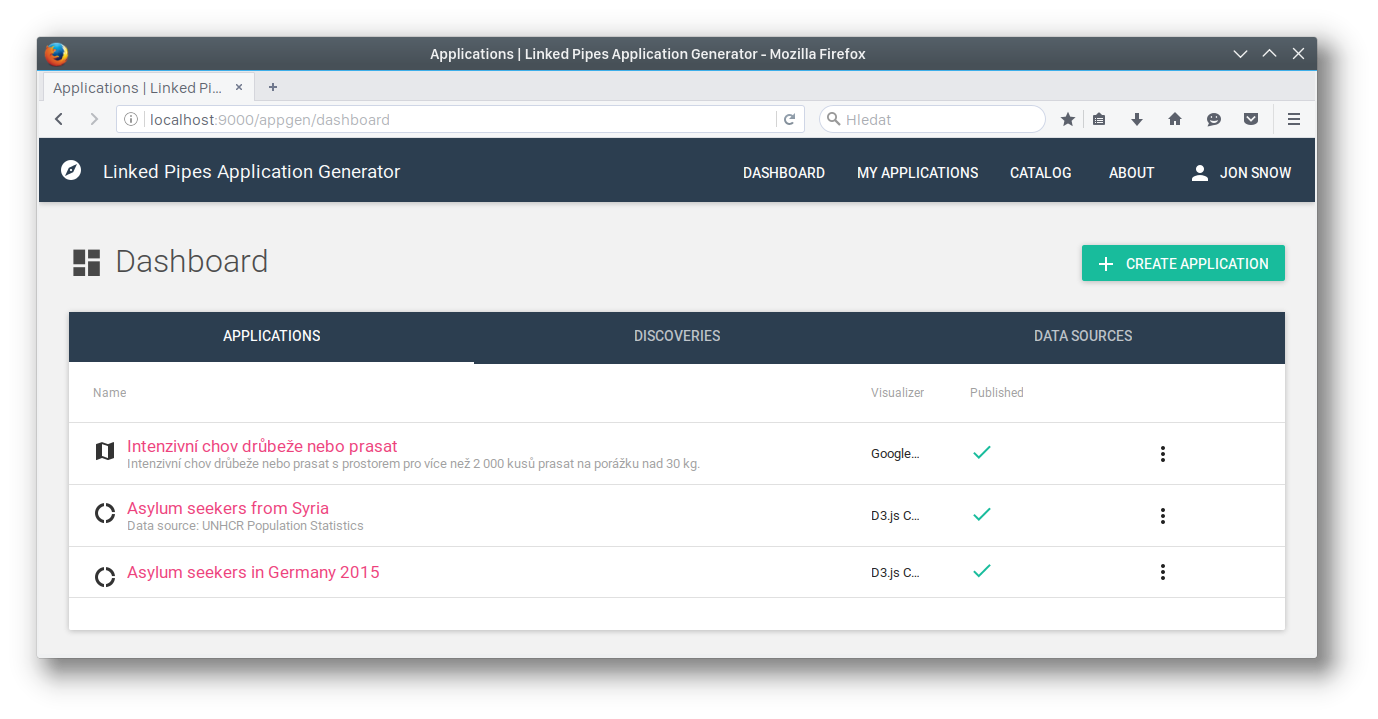
\includegraphics[width=145mm]{img/05_dashboard}
	\caption{User dashboard showing the overview of applications, discoveries and data sources}
    \label{fig:dashboard}
\end{figure}

\subsection{Data sources}

Our  approach to data sources is slightly different to LinkedPipes Visualization. In LinkedPipes Visualization, the user starts by providing the data source (may it be the SPARQL endpoint URL or a *.ttl file with serialized RDF data) and he has to do it every single time he wants to create a visualization. In our \emph{application generator}, we focused more on the possibility to re-use and share the data sets. So the user has to start by adding a data source to the generator, giving it a common name and only then he is allowed to select it for visualization. 

If we just have a new data set and want to get to a visualization quickly, the approach of LinkedPipes Visualization is faster. But once we want to re-use that data set, our approach wins over. 

That is not the only advantage. In our \emph{application generator}, we distinguish between public and private data sources. Private data sources are seen only by their owner (it should be mentioned that they are just hidden by the user interface, they are not actively protected from being used by other users). Public data sources, on the other hand, ale openly available for anyone and can be selected in the data source browser (Figure \ref{fig:scenario-01-browse-data-sources}). Any user can decide to make any of his data sources public. The idea is that one user (a data expert) might prepare the data set and another might use it to generate an application.

This approach introduces another level of abstraction. The user generating an application does not have to know what RDF or a SPARQL endpoint is, i.e, he is separated from the technical details. He can simply select the data source he is interested in from the browser and use it.

\subsection{Pipeline discovery}

The \emph{application generator} runs the underlying LDVM \emph{discovery} algorithm on the selected data sources. The \emph{discovery} returns all possible LDVM \emph{pipelines} that lead to a visualization, i.e., they end with a \emph{visualizer component}. Multiple \emph{pipelines} might use the same \emph{visualizer component} (they might use different \emph{analyzers} and \emph{visualizer transformers} along the way to get the input data compatible with this particular visualizer). Unfortunately, we are not able to give the user any detailed information about how the data produced by a \emph{pipeline} will look like. The only way to find out is to actually run the \emph{pipeline} and create an application from it. If the data do not make sense or are not what the user expects, he can try another one.

The user can watch the \emph{discovery} algorithm progress on a dedicated screen that shows the current \emph{discovery} status and also the list of \emph{pipelines} that have been discovered so far (Figure \ref{fig:scenario-02-discovery-result}). The \emph{pipelines} are grouped by \emph{visualizers}. As the algorithm may take some time, the user can leave the screen and come back later. It is accessible even after the \emph{discovery} algorithm finishes. The list of all discoveries can be found on the dashboard \ref{fig:dashboard}.

Note that not all \emph{visualizer} are supported by our \emph{application generator} (i.e., the corresponding \emph{plugin} is missing). For example, LinkedPipes Visualization contains a \emph{visualizer} for statistical data described using Data Cube Vocabulary \cite{datacube_vocabulary}. If the appropriate LDVM \emph{component} is registered in our \emph{application generator}, the \emph{discovery} algorithm will return \emph{pipelines} that use this \emph{component}. However, those will not be offered to the user.

\subsection{Application configuration}

The configuration phase is the core feature of the \emph{application generator} which differentiates it from the LinkedPipes Visualization. The application configuration involves both tasks that are common for all applications (e.g. publishing, deleting, updating description etc.) and that are \emph{visualizer} specific. As you can see on the Figure \ref{fig:configurator}, the \emph{configurator} interface follows this principle. It is divided into the common area and the area which is controlled by a particular \emph{visualizer} plugin (see Figure \ref{fig:google_maps_visualizer} of how a different \emph{visualizer} adapts to the universal configurator interface). 

\begin{figure}
	\centering
	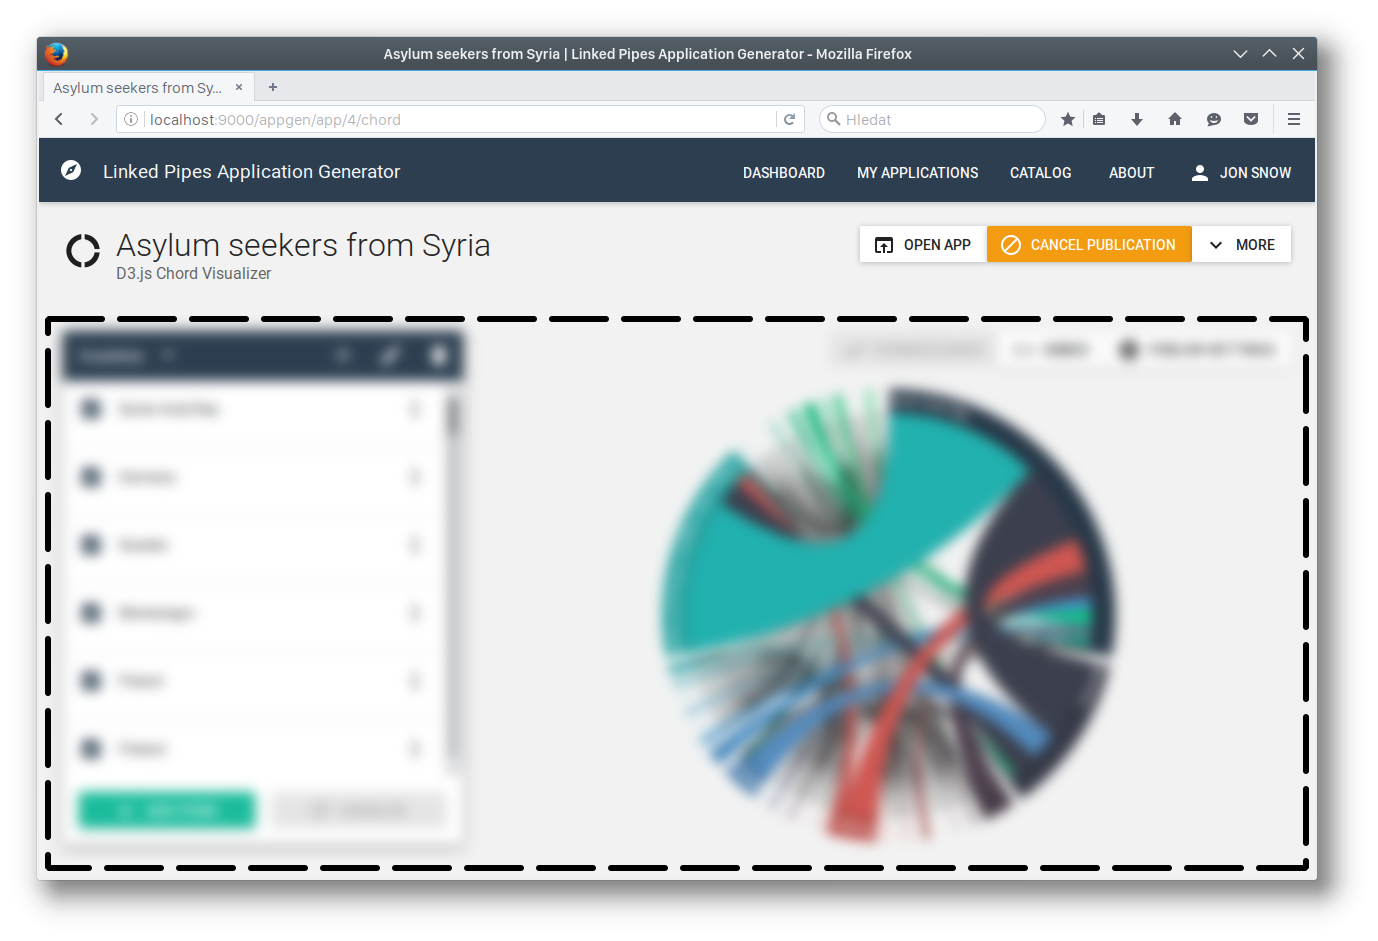
\includegraphics[width=145mm]{img/05_configurator.png}
	\caption{The configurator interface. The blurred out part is controlled by the current visualizer whereas the rest is identical for all visualizers. It contains the common functionality (e.g. the "More" button in the upper right corner shows a menu allowing the user to delete the application or change the application name and description).}
    \label{fig:configurator}
\end{figure}

\begin{figure}
	\centering
	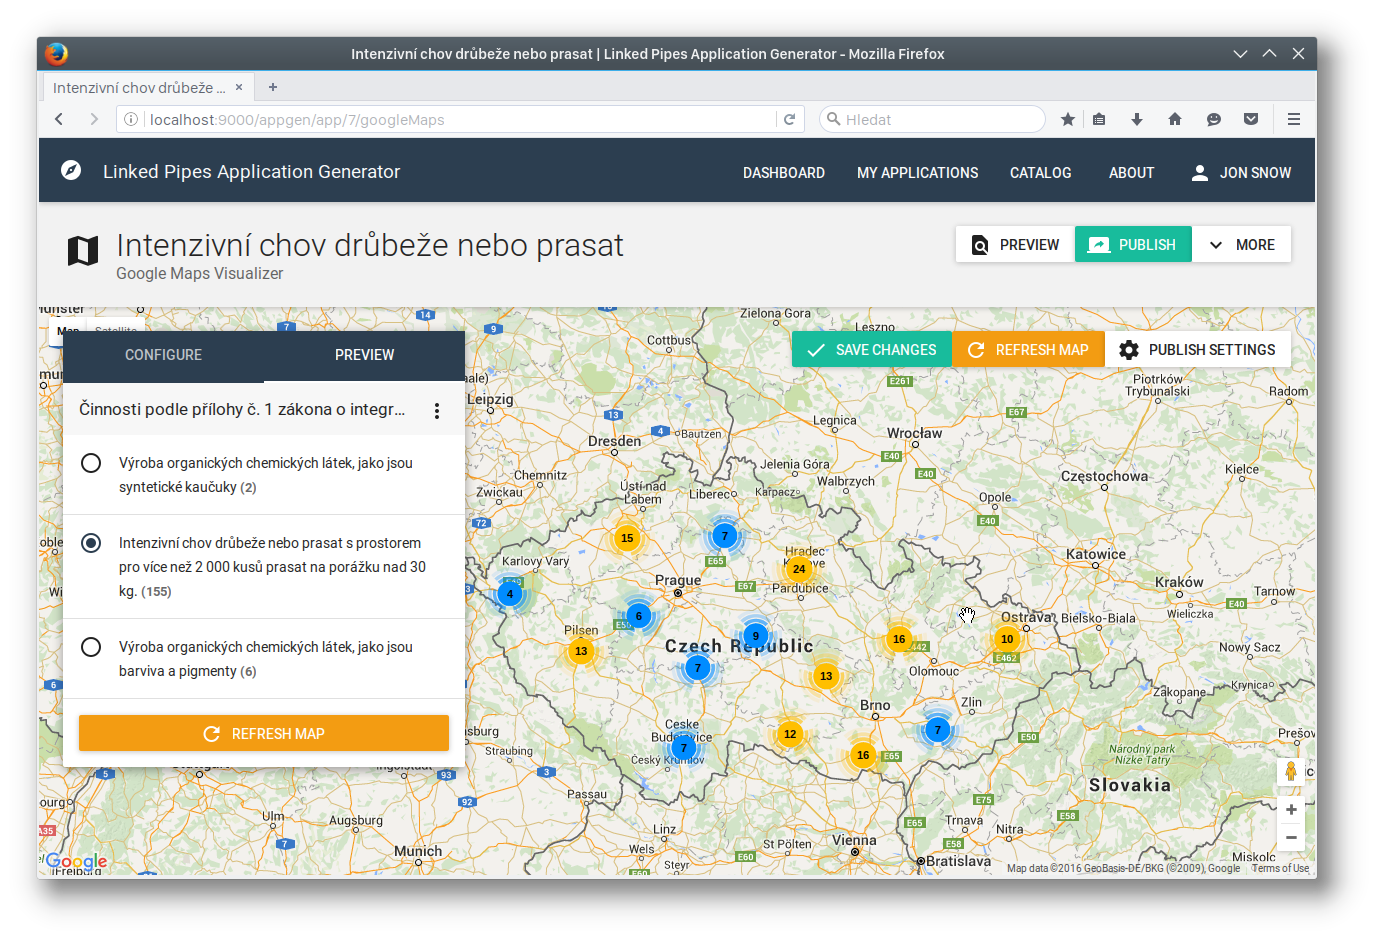
\includegraphics[width=145mm]{img/05_google_maps_visualizer.png}
	\caption{The configurator interface of the Google Maps Visualizer.}
    \label{fig:google_maps_visualizer}
\end{figure}

\subsection{Publishing applications}

When the user is happy with how the application looks, he can publish it by hitting the green "Publish button" (as seen for example on the Figure \ref{fig:scenario-04-graph-sample} in the upper right corner). The application then becomes accessible on a public URL which is generated from the application ID (internal numeric identificator) and its name. The \emph{application generator} at this moment does not offer any fine grained control of who gets to access the application. It is either public or not. Once it is published, it also becomes part of the public application catalog (Figure \ref{fig:catalog}).

\begin{figure}
	\centering
	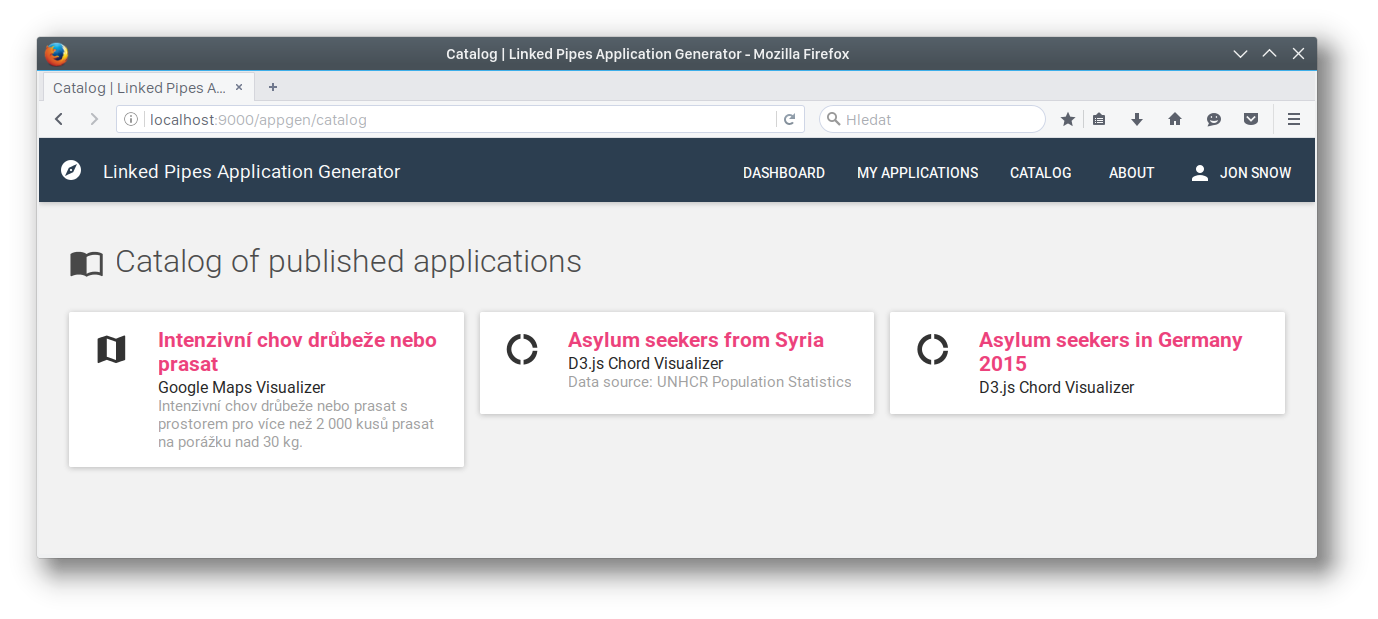
\includegraphics[width=145mm]{img/05_catalog}
	\caption{Catalog of published applications.}
    \label{fig:catalog}
\end{figure}

Some \emph{visualizers} offer the option to publish the application in an embed mode. That means that the application's interface is adapted so that it can be inserted for example into an external online article. The interface is usually significantly reduced and stripped from unimportant  control elements. This functionality is not considered common for all \emph{visualizers}  as each \emph{visualizer} can approach it differently. For example, the D3.js Chord Visualizer we used in this section allows the user to create multiple chord diagrams within a single application. Each of these diagrams can be exported separately in the embed mode (a unique URL is generated for each diagram under which the diagram is accessible). See Figure \ref{fig:scenario-10-embed-application}. Clearly, this functionality is specific for D3.js Chord Visualizer.

\section{General architecture}

We decided that we build our \emph{application generator} on top of LinkedPipes Visualization (Section \ref{sec:system_proposal:integration}). We already described the architecture of this tool (Section \ref{sec:linkedpipes:architecture} and especially Figure \ref{fig:linked-pipes-visualization-architecture}). We will now explain how we integrated the \emph{application generator} into LinkedPipes Visualization. You will get the overall idea by referring to Figure \ref{fig:application-generator-architecture}.

\begin{figure}
	\centering
	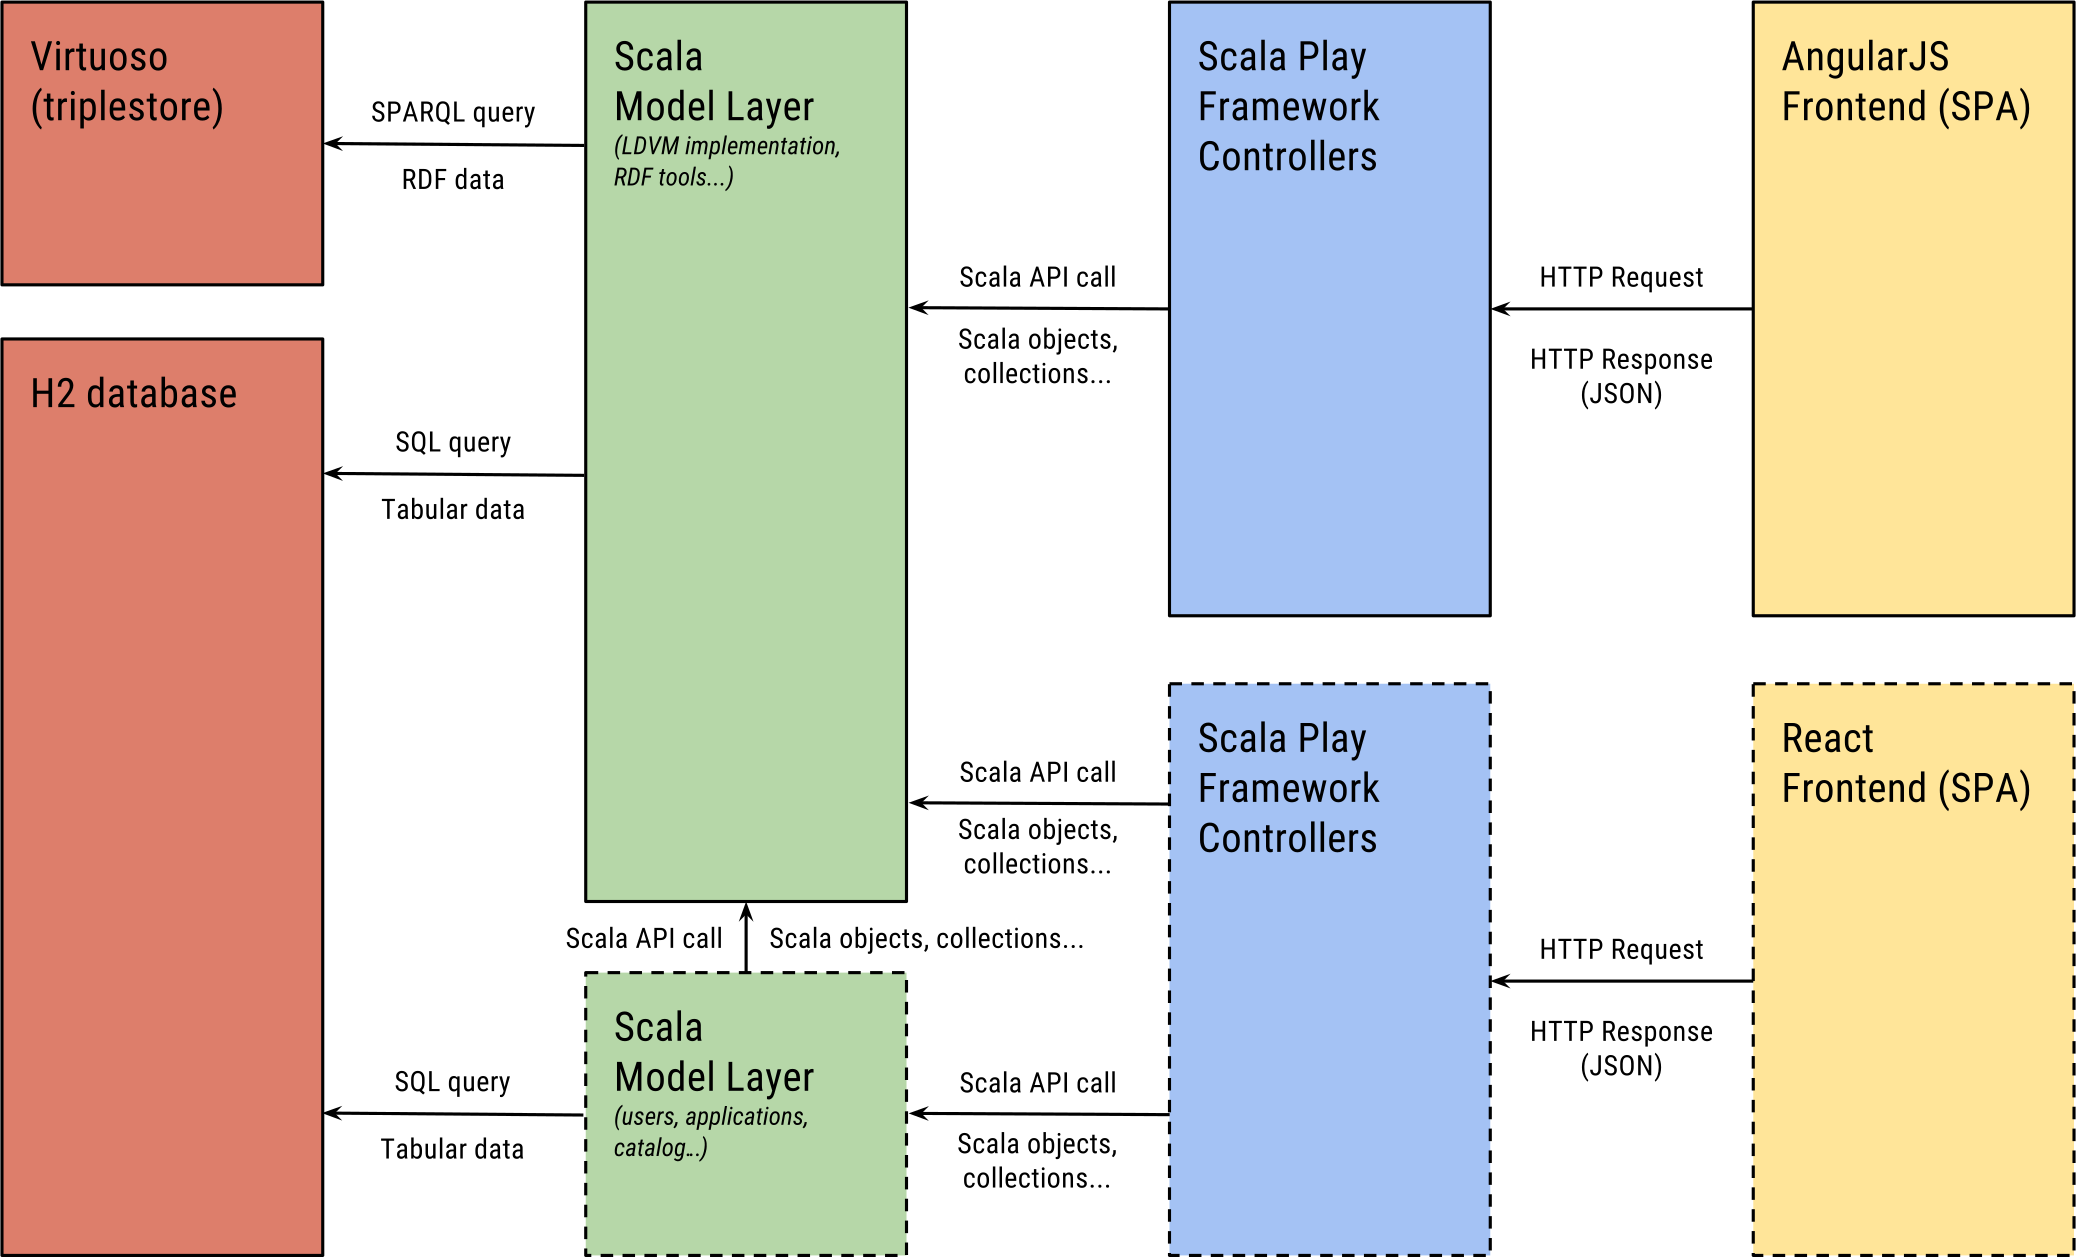
\includegraphics[width=140mm]{img/05_application_generator_architecture.png}
	\caption{Application Generator Architecture. Blocks with solid borders are part of the original LinkedPipes Visualization, blocks with dashed borders are newly implemented parts of the \emph{application generator}.} 
	\label{fig:application-generator-architecture}
\end{figure}

The \emph{application generator} is part of the original LinkedPipes Visualization code base. We made this decision after consulting the authors of LinkedPipes Visualization. From the software architectonic perspective, it is probably not the cleanest approach, but it significantly sped up our work. The original code base contained many solutions and APIs that we could immediately use (for example the LDVM implementation API, various RDF tools etc.). Nevertheless, even though both tools live in the same code base, we made sure to keep them as separated as possible (Figure \ref{fig:application-generator-architecture} shows that clearly). So if we decided in the future to separate both tools or for example replace the underlying LDVM implementation, it should not be impossible.

An important consequence of this unification is that the LDVM implementation instance is shared among the \emph{application generator} and LinkedPipes Visualization. That means that they both use the same set of registered LDVM \emph{components}. We benefited from this as well to an extent. Due to the lack of time, we did not manage to implement all user interfaces for our generator. For example, new LDVM \emph{components} are registered to the \emph{generator} through the LinkedPipes Visualization user interface.

\subsection{Frontend}

The \emph{application generator} frontend is completely new and independent on the original frontend. The original frontend already contained some work that we could at first glance use (e.g. existing \emph{visualizer} plugins). Unfortunately, couple of problems prevented us from doing so. Firstly, the AngularJS frontend was created just to showcase the capabilities of the underlying LVDM implementation. For this reason, its code was in a rather poor state with no documentation. Clearly, it would take us lots of time to get familiar with it. Secondly, this code was not written with certain features (like for example user support) in mind. Thirdly, our \emph{visualizers} (with the separated \emph{configurator} and \emph{application} interfaces) work very differently compared to the \emph{visualizers} of LinkedPipes Visualization. Having these three reasons in mind, we came to the conclusion that we would have to rewrite a major portion of the original code anyway and therefore we decided to start from the scratch. We also decided to go with a different development stack (we replaced AngularJS with React and related tools) which we believed would fit our needs better. 

As a result, there are two existing user interfaces that live within the same application next to each other. The original LinkedPipes Visualization interface is accessible from the home page (the \texttt{/} URL). Our \emph{application generator} can be found at \texttt{/appgen} and individual published applications live at \emph{/app}.

\subsection{Controllers}

The vast majority of controllers in both LinkedPipes Visualization and the \emph{application generator} handle the asynchronous HTTP requests coming from the frontend (the only exception are the controllers handling the initialization of the SPAs). The role of a controller in this typical case is just to translate the HTTP request into an API call to the \emph{Model} layer and send the response back. All controllers together define a public remote API interface.

Even though we could re-use some of the methods available from the LinkedPipes Visualization controllers (e.g. those for controlling the \emph{discovery} algorithm), we decided not to do that to avoid hidden dependencies between the frontend and the backend. Dependencies within the Scala code base (for example between the \emph{Controller} layer and the \emph{Model} layer) are easy to discover. If they break, the code will not compile. That is not true for the remote API. Therefore the \emph{application generator} frontend strictly uses only those remote API methods that are handled by the \emph{application generator} controllers. They all exist in a standalone \texttt{controllers.appgen} Scala package.

\subsection{Model}

The \emph{Model} layer consists of various repositories and services that handle the business logic. The repositories and services that specifically handle the \emph{application generator} business logic (e.g. application management, users etc) can all be found in the \texttt{model.appgen} package.

The \emph{Model} layer among other things contains tools for working with RDF data, e.g. services converting RDF data in various vocabularies into Scala objects. While we were developing our \emph{visualizers}, we needed to add support for some new vocabularies to the code base. This is the only case when our code significantly overlaps with the original LinkedPipes Visualization code. However, this code is not specific to our \emph{application generator}, it actually extends the functionality of LinkedPipes Visualization.

Figure \ref{fig:application-generator-architecture} might suggest that our extension of the \emph{Model} layer directly communicates with the H2 database. Strictly speaking, that is not true because we are utilizing some low level services to access the database and those services could still be considered part of the \emph{Model} layer.

What is important is that all \emph{application generator} related Scala code exists in those two packages (\texttt{controllers.appgen} and \texttt{model.appgen}). Also the frontend strictly communicates only  with our controllers. Therefore it is easy to draw the line where LinkedPipes Visualization ends and our \emph{application generator} begins. Dependencies between our code and the original code base are shown on Figure \ref{fig:application-generator-architecture} and are always a matter of Scala code. The dependencies are in a form of utilizing the internal API of LinkedPipes Visualization. In rare cases, we re-use some low-level utilities from the original code base.

\section{Frontend development stack}
\label{sec:implementation:frontend-development-stack}

One of the goals of this chapter is to convince the reader that our \emph{application generator} can work as a \emph{framework} for developing new \emph{visualizers}. For that we need the reader to understand the \emph{application generator} on a code level. The backend architecture is fairly standard and especially the integration is simple. Most of the work happens in frontend which uses a development stack that is rather new and very specific. In this section, we will try to explain the reader the core frontend technologies that we use so that he can later understand the integration process of a new \emph{visualizer}. The information that we are about to provide here is in no way related directly to the \emph{application generator}. It will be a short extract from the documentations of these tools and we will only aim to provide just enough information so that the reader can understand our code. Anyone who feels already familiar with these tools, can skip this part.

\subsection{ES6 and Babel compiler}

The frontend is completely written using ECMAScript 2015 \cite{es6} (known as ES6) which is the 6th version of ECMAScript standard. JavaScript is an implementation of ECMAScript, available in all mainstream browsers. ES6 introduces many new language constructs which are, however, not all supported by the current JavaScript implementation. We use Babel \footnote{https://babeljs.io/} transpiler which converts our ES6 code into standard JavaScript.

We will mention some of the features that we frequently use.

\begin{verbatim}
// Arrow functions
[1, 2, 3].map(x => x * x);

// var is replaced with const (for constants) and let (for mutable variables)
const PI = 3.14;
let i = 1;
i++;

// Standard class syntax (the prototypical inheritance is still under the hood)
class Dog extends Animal {
  constructor(name) {
    super(name);
  }
}

// Enhanced Object Literals
const a = 2;
const b = 3;
const obj = { a, b };
obj.a === 2;
obj.b === 3;

// Desctructing
const obj = { a: 2, b: 3 };
const { a, b } = obj;
a === 2;
b === 3;

const arr = [1, 2, 3];
const [a, b] = obj;
a === 1;
b === 2;
\end{verbatim}

Perhaps the most important feature for us are ES6 modules. Each file is a module which \emph{imports} its dependencies and \emph{exports} values that make a public API of that module.

\begin{verbatim}
// lib/math.js

export const PI = 3.14;

export function add(a, b) {
  return a + b;
}

export const multiply = (a, b) => a * b;

export default { add, multiply, PI };
\end{verbatim}

There are several ways how a dependency can be \emph{imported}.

\begin{verbatim}
import { multiply, PI } from './lib/math'

const result = multiply(PI, 2);
\end{verbatim}

\begin{verbatim}
import * as math from './lib/math'

const result = math.add(math.PI, 2);
\end{verbatim}

\begin{verbatim}
import math from './lib/math'

const result = math.add(math.PI, 2);
\end{verbatim}

\subsection{npm}
npm \cite{npm} is a package manager for JavaScript. We use it to manage our JavaScript dependencies. They are all listed in the file \texttt{src/package.json}. Once installed, a package can be used with the standard \texttt{import} command.

\begin{verbatim}
import moment from 'moment'

moment().format('MMMM Do YYYY, h:mm:ss a'); // prints current time and date, i.e. June 24th 2016, 8:52:00 pm
\end{verbatim}

Note that when importing a npm dependency, we do not use relative paths starting with a dot.

\subsection{React}
React \cite{react} is a JavaScript library for building user interfaces. The base building block is a React component.

\begin{verbatim}
import React from 'react'

const HelloMessage = ({ name }) => (
    <div>Hello <strong>{name}</strong></div>
  )

React.render(<HelloMessage name="Jon Snow" />, document.getElementById('container'));
\end{verbatim}


This is the simplest shortest example possible where a component works as a plain function. It takes some input data and prints user interface. The input data are in the form of \texttt{props} which are passed in the first argument (we use ES6 destructing to extract the name \texttt{prop}). The user interface is defined using a XML-like syntax called JSX. This component prints a greeting with the highlighted name. Using the last line, the component is mounted to a specific DOM node marked with an id equal to "container".

The components can be composed. 

\begin{verbatim}
const HelloMessage = ({ name }) => (
    <div>Hello <strong>{name}</strong></div>
  );
  
const MessageList = ({ names }) => (
    <ul>
      {names.map(name => 
        <li>
          <HelloMessage name={name} />
        </li>
      )}
    </ul>
  )

const names = ['Jon Snow', 'Tyrion'];
React.render(<MessageList names={names} />, document.getElementById('container'));
\end{verbatim}

This example will print a greeting for each name in the list. As you can see, we can easily combine HTML tags with our own components. The \texttt{props} are passed down to the components with the syntax that we use for specifying  standard HTML attributes.

The components can be interactive.

\begin{verbatim}
class Counter extends React.Component {
  constructor(props) {
    this.state = {
      value: props.initialValue
    }
  }
  
  increase() {
    this.setState({
      value: this.state.value + 1
    })
  }
  
  render() {
    const { value } = this.state;
    return (
      <input type="button" 
        onClick={() => this.increase()} 
        value={'Increase: ' + value} />
     );
  }
} 

React.render(<Counter initialValue={10} />, document.getElementById('container'));
\end{verbatim}

This component no longer works as a simple function as it maintains its own state. The state contains just a numeric value which is increased every time the user click the button. The value is displayed in the input label. Note that we cannot simply assign the new value to the \texttt{state} object, we need to use the \texttt{setState} method which is part of the React API.

In this case, the rendered UI is a function of the component \texttt{props} and the component \texttt{state}. Whereas the \texttt{props} are immutable (like function arguments), the \texttt{state} can be mutated within the component.

In React, \textbf{you do not mutate the user interface}. That means that you do not define how the user interface should transition between different states but instead, you specify how the interface should look like given the current \texttt{props} and \texttt{state}. Every time the \texttt{state} changes or new \texttt{props} are passed from the parent component, the whole UI is completely re-rendered. This significantly simplifies building interactive user interfaces. If nothing else, the number of possible component states is significantly lower than the number of possible transitions between those states.

The React API defines several life cycle methods.

\begin{verbatim}
class GreetOnMount extends React.Component {
  componentWillMount() {
   alert('This component is about to be mounted to the DOM tree!');
  }
  
  componentWillUnmount() {
   alert('This component is about to be unmounted from the DOM tree!');
  }
  
  render() {
   return <div />
  }
}
\end{verbatim}

We have used two life cycle methods, \texttt{componentWillMount} which is triggered when the component is about to appear, and \texttt{componentWillUnmount} which is triggered when the component is about to disappear from the screen. These methods are especially useful for components that fetch data from the server. The first method can be used to initiate the request and the second method to cancel the request or possibly do some cleaning up.

\subsection{Redux}
\label{sec:implementation:frontend-development-stack:redux}

If we were to use the MVC terminology, we would say that a React component is a \emph{controller-view}. It both handles the interaction with the user and the visual representation. In our code, we usually try to distinguish between controllers and views. We create either a component that is rather a controller, i.e., it handles user input but does not focus on the visuals, or a component that is rather a view, i.e., there is no business logic going on and the component focuses only on representing the data on the screen. By composing components of these two types we build the whole user interface.

The component state fits the definition of the \emph{Model} layer. Nevertheless, this approach, i.e., storing everything in the state of React components, would not work for large-scale applications which would have a lot of state. The \emph{state} in this context can mean literary everything, starting all the data fetched from the server, ending with the list of open dialog windows. That is why we use Redux.

Redux \cite{redux} is, as explained by the authors, a "predictable state container for JavaScript apps" that evolved from the Flux ideas. Flux \cite{flux} is an application architecture that was designed specifically to work with React applications. Even though Redux is independent on React, they work extremely well together. 

Setting up Redux with React is a bit complicated so we skip it. It is not really necessary because it is already done for us in the fronted code base and we can immediately start using it. The more important thing is to understand how it works.

The core idea is that we move the state out of the components. Let us start with a simple example. Our \emph{state} will be just a single number. We want to be able to increment and decrement the number. For each such operation we create an \emph{action type}.

\begin{verbatim}
const INCREMENT = 'INCREMENT';
const DECREMENT = 'DECREMENT';
\end{verbatim}

It is good practice that we also define \emph{action creators}.

\begin{verbatim}
function increment() {
  return { type: INCREMENT };
}

function decrement() {
  return { type: DECREMENT };
}
\end{verbatim}

Now we define a special function called a \emph{reducer} which specifies how every \emph{action} transforms the \emph{state}.

\begin{verbatim}
function valueReducer(state = 0, action) {
  switch (action.type) {
    case INCREMENT:
      return state + 1
    case DECREMENT:
      return state - 1
    default:
      return state
  }
}
\end{verbatim}

The function takes the current \emph{state} and an \emph{action} as an argument. Depending on the \emph{action type} (and typically also \emph{action payload}), it transforms the \emph{state}. What is important is that the function does not mutate the old \emph{state} but rather creates a completely new \emph{state} from the old \emph{state}. In this case the \emph{state} is just an integer which is by its nature immutable. If the \emph{state} was more complex, typically an object, we would need to make sure to create a new object  every time it changes.

From a \emph{reducer} we create a \emph{store} which represents a running instance of Redux. It holds the current \emph{state} and provides a \emph{dispatch} function that we use to apply the \emph{actions} on the \emph{state}.

\begin{verbatim}
dispatch(increment());
dispatch(decrement());
\end{verbatim}

Now let us see how we bind this to a React component.

\begin{verbatim}
import React from 'react'
import { connect } from 'react-redux'

const Counter = ({ dispatch, value }) => (
  <div>
    {value}
    <input type="button" onClick={() => dispatch(increase())} label="Increase" />
    <input type="button" onClick={() => dispatch(decrease())} label="Decrease" />
  </div>
);

const mapStateToProps = state => ({
  value: state
});

export default connect(mapStateToProps)(Counter);
\end{verbatim}

This way we \emph{connected} the component to the \emph{store}. The \emph{dispatch} function is automatically injected to the component as a \emph{prop} which means that we can start \emph{dispatching} actions to modify the \emph{state}. The \emph{state} (in our case just a single integer) is also injected to the component through the \emph{props} but we have to specifically define how that should happen using the \texttt{mapStateToProps} function.

The process makes up a circle. The user clicks the button in the component and an \emph{action} is \emph{dispatched} to the \emph{reducer}. The \emph{reducer} updates the \emph{state} and the \emph{store} notifies the component of a change. The component re-renders with the updated value. As the \emph{state} can be changed only using \emph{actions}, the system behavior is predictable and very explicit. Redux offers a development mode in which it is very easy to monitor the \emph{actions} flowing through the system and how they change the \emph{state} (Figure \ref{fig:graph-visualizer}).

The \emph{reducers} can be composed and combined. Let us now add another reducer that will simply count the number of clicks.

\begin{verbatim}
function clickCountReducer(state = 0, action) {
  switch (action.type) {
    case INCREMENT:
    case DECREMENT:
      return state + 1
    default:
      return state
  }
}
\end{verbatim}

Now we combine the reducers together.

\begin{verbatim}
import { combineReducers } from 'redux'

const rootReducer = combineReducers({
  value: valueReducer,
  clickCount: clickCountReducer
});
\end{verbatim}

This creates a new \emph{reducer} that combines the other two \emph{reducers} together in a way that it maintains two values in an object where each value is updated by the corresponding \emph{reducer}. Whenever an \emph{action} is \emph{dispatched}, the root \emph{reducer} passes the \emph{action} to both child \emph{reducers}.

Suddenly, our \emph{state} is more complicated because it is an object with two values. We have to update the \texttt{mapStateToProps} function accordingly.

\begin{verbatim}
const Counter = ({ dispatch, value, clickCount }) => (
  // ...
);

const mapStateToProps = state => state;
\end{verbatim}

In this case, we could actually significantly simplify the function as the \emph{state} structure directly corresponds to the \emph{props} that we want to inject.

In a similar manner we could start adding more and more \emph{reducers} to fit the needs of the application (and the \emph{state} hierarchy would grow correspondingly). Our \emph{application generator} has only one single vast and deep \emph{state} that holds all the information. If we apply the React component hierarchy on this \emph{state} hierarchy (updated by the \emph{reducer} hierarchy), we get the user interface that is currently on the screen.  We can say that what you can see on the screen is a \emph{function} of the \emph{state}.

% TODO: show action creators using promises and thunks

\subsection{Reselect}

We use the \texttt{mapStateToProps} function to extract the values from the \emph{state} required by a component. That worked really well for our simple examples but  it would not scale with the increasing size and depth of the \emph{state} object.

The \emph{state} can be viewed as a database. It is a huge blob of data that any part of the application can access. It defines a clear API for making updates and the updates are always performed in transactions (that stems from the single-threaded nature of JavaScript but what also matters is that when an \emph{action} is \emph{dispatched}, it has to update all \emph{reducers} first before another \emph{action} can be \emph{dispatched}). What we miss is an API for selecting data from the database, i.e., the \emph{state}. We use Reselect \cite{reselect} for that.

We will re-use the last iteration of our example with the \texttt{valueReducer} and \texttt{clickCountReducer}.

\begin{verbatim}
import {  createStructuredSelector } from 'reselect'

// ... the component

const valueSelector = state => state.value;
const clickCountSelector = state => clickCount;

const selector = createStructuredSelector({
  value: valueSelector,
  clickCount: clickCountSelector
});

export default connect(selector)(Counter);
\end{verbatim}

A Reselect \emph{selector} is like a named database query. It extracts a specific piece of data from the \emph{state}. We defined two base \emph{selectors} that access directly the state and we combined them together. Our final \emph{selector} becomes the \texttt{mapStateToProps} function. What is important is that once a \emph{selector} is created, we do not have to care about how it is implemented. For us, it is just a query that returns the data we need. That separates us from the raw \emph{state} structure. Just like we have a \emph{reducer} hierarchy and a \emph{component} hierarchy, we can add a \emph{selector} hierarchy covering the whole \emph{state}.

Let us say that \texttt{state.auth.user.id} contains the ID of the currently authenticated user. We want to inject that ID into a component. This is the simple \texttt{mapStateToProps} approach:

\begin{verbatim}
const mapStateToProps = state => ({
  userId: state.auth.user.id
});
\end{verbatim}

With a smart \emph{selector} hierarchy, we could do this.

\begin{verbatim}
import { createSelector } from 'reselect'
import { userSelector } from './selectors'

const selector = createSelector(
  [userSelector],
  user => ({ userId: user.id }));
\end{verbatim}

Whereas in the first example, we actually have to know the complete \emph{state} hierarchy to extract this piece of information (and that can very often change due to refactoring), in the second example we are completely separated from the \emph{state} hierarchy and we just need to know the schema of the user object that the \texttt{userSelector} returns.

The selectors can do some extra calculations. Using a simple math formula we calculate the number of increment clicks. Clearly, we could maintain this information in another \emph{reducer} but as we can derive this information from information that is already in the state, it would be duplication.

\begin{verbatim}
const incrementCountSelector = createSelector(
  [valueSelector, clickCountSelector],
  (value, clickCount) => (clickCount + value) / 2);
\end{verbatim}

The \emph{selectors} can be arbitrarily combined.

\begin{verbatim}
const decrementCountSelector = createSelector(
  [clickCountSelector, incrementCountSelector],
  (clickCount, incrementCount) => clickCount - incrementCount);
\end{verbatim}

Every time the \emph{state} is updated, the \emph{selectors} are recalculated and consequently the \emph{components} are re-rendered. The \emph{selectors} are actually slightly smarter than that. The \emph{selector} output is automatically cached and if its input does not change, the cached value is returned instead. Therefore the \emph{selectors} can be used even for heavy computations.

\subsection{React-router}

As one would expect, our \emph{application generator} will consist of many different screens with different functionality. We need a mechanism for transitioning between those screens. Although many approaches are viable, we prefer the one with classic URLs, i.e., every different screen has its own URL. It has clear benefits as the user navigates through the interface as if it was a standard web page (e.g. even with the back button support).

Our \emph{application generator} is a SPA which means that each URL will contain the part corresponding to the actual physical address of the SPA (the entry URL) and the part maintained only by the frontend JavaScript application.

\begin{verbatim}
Sample URL: 
http://localhost:9000/appgen/dashboard/discoveries

SPA entry URL: 
http://localhost:9000/appgen/

Virtual URL part maintained by the SPA: 
dashboard/discoveries
\end{verbatim}

JavaScript API in modern web browsers allows us to change the URL without actually reloading the page.

We use React-router \cite{react-router} as a routing library for React. To show you how it works, we borrow an example from their documentation.

\begin{verbatim}
import React from 'react'
import { Route, IndexRoute } from 'react-router'

const App = ({ children }) => (
    <div>
      <h1>Welcome to our app</h1>
      {children}
    </div>
  );

const About = () => <h2>About</h2>

const Users = ({ children }) => (
    <div>
      <h2>Users</h2>
      {children}
    </div>
  );

const User = ({ params: { userId }}) => <div>User: <strong>{userId}</div>

const NoMatch = () => <h2>Not found</h2>

const routes = (
    <Route path="/" component={App}>
      <Route path="about" component={About}/>
      <Route path="users" component={Users}>
        <Route path=":userId" component={User}/>
      </Route>
      <Route path="*" component={NoMatch}/>
    </Route>
  );
\end{verbatim}

The React-router uses JSX for routes definition which makes it very declarative. For each route, we define a React component that is activated when the URL matches this particular route. The URL segment that has to be matched is defined by the \texttt{path} attribute, the component by the \texttt{component} attribute. The routes definition is hierarchical specifying the complete URL schema.

When a URL is matched, all components along the path of matching routes through the routes definition are activated. For example, for the URL \texttt{/users/15} the components \texttt{App}, \texttt{Users} and \texttt{User} are activated. The child component is always passed to the parent component through the \texttt{children prop}. 

As you might have noticed, all the tools in our stack introduce some kind of explicit composability. That is very useful because it will make all parts of our  \emph{application generator} easily extendable and re-usable.

\subsection{Immutable.js}

Immutable.js \cite{immutable} is a library containing  standard data structures that we may know for example from Java (e.g. \texttt{List}, \texttt{Map} or \texttt{Stack}). The core feature is that all the data structures are \emph{immutable} which means that they cannot be changed. If we change an instance of a \texttt{List} (e.g. by adding an element) we create a completely new instance and the old one remains unchanged. Consider the following example.

\begin{verbatim}
import { List } from 'immutable'

const list = new List();
const listUpdated = list.push(5);

list.size === 0;
listUpdated.size === 1;
\end{verbatim}

This library has many advantages. Firstly, it provides an extremely strong and well documented API which goes beyond the capabilities of standard JavaScript collections (\texttt{object} or \texttt{array}). The API fits better into the functional nature of our code. Secondly, it works really well with \emph{reducers}. As explained, a \emph{reducer} has to always return a new state which is sometimes a bit complicated using the standard JavaScript API. In the following example, we need to create a new copy of an object containing users identified by their IDs.

\begin{verbatim}
function usersReducer(state = {}, action) {
  switch (action.type) {
    case ADD_USER: 
      return Object.assign({}, state, {
        action.payload.id: action.payload.id
      })
    default:
      return state;
  }
}
\end{verbatim}

Now consider the version with Immutable.js.

\begin{verbatim}
import { Map } from 'immutable'

function usersReducer(state = new Map(), action) {
  switch (action.type) {
    case ADD_USER: 
      return state.set(action.payload.id, action.payload.id);
    default:
      return state;
  }
}
\end{verbatim}

Thirdly, there are some speed benefits as this is what makes the Reselect caching actually possible. A \emph{selector} recalculates only when the input arguments change. If an input argument was a standard mutable object, it would be very complicated (and expensive) to determine whether it changed. We would be keeping a reference to that object and have no idea whether the object was changed in the mean time. On the other hand, if we keep a reference to an immutable structure and the reference does not change, then we can be sure that the content of the referenced structure also did not change and we can re-use the cached value. Similar mechanism is used also for React components, i.e., it is possible to avoid unnecessary re-renders.

Lastly, Immutable.js library offers the \texttt{Record} data structure which is essentially a \texttt{Map} (i.e., a \emph{key-value} storage, just like a standard JavaScript \texttt{object}) but with an enforced schema.

\begin{verbatim}
const User = Record({
  id: 0,
  name: 'Anonymous user'
});

const user = new User({ id: 5, gender: 'male' });

user.id === 5;
user.name === 'Anonymous user';
user.gender === null;
\end{verbatim}

Any values that are missing during the instantiation are replaced with the default values and any values that are not part of the schema are removed. Unlike the standard immutable \texttt{Map}, a \texttt{Record} properties can be accessed using the standard dot notation (it even supports destructing). It is also very useful when we are defining the \texttt{propTypes} of a React component.

\begin{verbatim}
class UserView extends React.Component {
  static propTypes = {
    user: React.PropTypes.instanceOf(User).isRequired
  }
}
\end{verbatim}

If this component does not receive a \texttt{User} instance through the \texttt{props}, a warning is thrown.

\section{Frontend framework architecture}

In this section, we will give the reader a brief overview of the  overall structure of the frontend code and we will also explain several design ideas that are specific to our code. In the previous section (Section \ref{sec:implementation:frontend-development-stack}) we described several tools that together make up the development stack that we use. Clearly, there is no monolithic framework. Each tool solves only one problem and even though they have been all designed to work well together and complement each other, there is missing an overall architecture and design patterns for large scale applications (something that a well-established monolithic framework usually offers).

There exist recommendations and patterns but they evolve just as quickly and erratically as the modern world of JavaScript frontend itself. While developing the \emph{application generator} (and making it a \emph{framework}) we had to choose the right patterns for us and sometimes even come up with some new patterns on our own.

This involves literary everything from the very basic questions of how our code should be organized to which library should we use to generate forms or how we should implement visual feedback for asynchronous requests. In this section we will focus mainly on the basic aspects which involve the code organization. It will all become useful when we start integrating our own \emph{visualizer}.

\subsection{JavaScript bundles}

As explained, our frontend code is written in ES6 and has to be compiled (or more correctly \emph{transpiled}) into standard JavaScript that any browser can understand. The frontend code base consists of large amount of (not only) ES6 files which are all transpiled and put together into a single JavaScript file which we call a \emph{bundle}. This bundle is loaded to the web browser and contains everything that is required to run the SPA. We use Webpack bundler \footnote{http://webpack.github.io/} to put our code together and Babel \footnote{http://babeljs.io/} transpiler to convert our code.

The disadvantage of this approach is that this bundle is typically very large and therefore takes some time to load. Before it loads, the user does not see anything on the screen. On the other hand, once it is loaded, the user experience is very smooth because we do not have to make any more request to the server to fetch additional resources.

Our \emph{application generator} consists of several bundles. The main is the \emph{platform} bundle which contains the whole \emph{platform} user interface and also \emph{configurator} interfaces for all registered \emph{visualizers}. Then every registered \emph{visualizer} has its own bundle that contains only the \emph{application} interface. This bundle is used for published applications and as it does not contain the whole platform, it is significantly smaller and faster to load.

Even though we have multiple bundles, all the code exists in one spot. The reason is that there is very little code that is used only in a single bundle and therefore it would not make sense to separate it in any way. What defines a bundle is an \emph{entry point} which is a simple JavaScript file where Webpack starts the bundling process.

\subsection{Code structure}

The frontend code is all in the folder \texttt{src/app/assets\_webpack/appgen}. We will refer to this folder as to the \texttt{assets} folder. There are two subfolders \texttt{javascripts} and \texttt{stylesheets} with self-explanatory names. What is interesting is that the styles are also included into the bundle.  Let us now quickly walk through the folders in \texttt{javascripts}.

\begin{itemize}
\item \textbf{components} -- useful single-purpose React components
\item \textbf{containers} -- the top level React components that are connected to Redux
\item \textbf{entries} -- Webpack entry points (each file here corresponds to a bundle)
\item \textbf{misc} -- various utilities
\item \textbf{modules} -- the actual code
\item \textbf{store} -- instantiation of Redux \emph{store}

\end{itemize}
\subsection{Ducks}

Our code contains lots of Redux \emph{actions}, \emph{reducers} and Reselect \emph{selectors}. A common pattern is to put all \emph{actions} into the \texttt{actions.js} file, all \emph{reducers} into the \texttt{reducers.js} file and all selectors into a \texttt{selectors.js} file. In our \emph{application generator}, we decided to adopt the \emph{duck} format \footnote{https://github.com/erikras/ducks-modular-redux}. The idea is that we put all \emph{actions}, \emph{reducers} and \emph{selectors} related to the same functionality into a single file called a \emph{duck}. 

We take the example from Section \ref{sec:implementation:frontend-development-stack:redux} where we were explaining how Redux works and rewrite it into the duck format. This would be a single file (i.e., an ES6 module).

\begin{verbatim}
// Actions 

export const INCREMENT = ’INCREMENT’;
export function increment() {
  return { type: INCREMENT };
}

export const DECREMENT = ’DECREMENT’;
export function decrement() {
  return { type: DECREMENT };
}

// Reducer

export default function valueReducer(state = 0, action) {
  switch (action.type) {
    case INCREMENT:
      return state + 1
    case DECREMENT:
      return state - 1
    default:
      return state
    }
}

// Selectors

export const valueSelector = state => state.value;
\end{verbatim}

This \emph{duck} covers the complete functionality regarding incrementing and decrementing a value. It exports public API for updating the value (\emph{action creators}), reading the value (\emph{selectors}) and it defines how the value should be represented and updated (\emph{reducer}). The \emph{action types} are exported as well which means that anyone can listen to these \emph{dispatched} \emph{actions}. In \emph{object-oriented programming} terminology we could say that the \emph{action creators} correspond to object \emph{setters} and \emph{selectors} to object \emph{getters}.

\subsection{Modules}

Clearly, having all React components and all \emph{ducks} in a single place is not viable for large applications. Therefore we introduce a \emph{module} which is the base organization unit in our code (please do not confuse it with ES6 modules). A \emph{module} is similar to a \emph{package} from Java. It usually covers one area of functionality. For example, we have an \texttt{auth} \emph{module} that covers everything related to authenticating and registering users. Also every registered \emph{visualizer} has its own \emph{module}.

A \emph{module} is in the first place a folder with standardized content. Let us walk through folders that a \emph{module} typically contains.

\begin{itemize}
\item \textbf{components} -- React components that focus mainly on the visuals (\emph{view} components)
\item \textbf{containers} -- React components that are connected to Redux and handle business logic (\emph{controller} components)
\item \textbf{dialogs} -- React components for dialog windows
\item \textbf{ducks} -- \emph{ducks} required in this module
\item \textbf{misc} -- various utilities
\item \textbf{pages} -- React components that are bound to React-router routes
\end{itemize}

All \emph{action types} in one \emph{module} should have a common prefix corresponding to the \emph{module} name. Firstly, when an \emph{action} is dispatched, we can easily identify which \emph{module} it came from. Secondly, we do not have to worry about conflicting \emph{action types} (with the prefix we are creating a separated namespace). Therefore each \emph{module} should contain a \texttt{prefix.js} file.

\begin{verbatim}
// prefix.js

import createPrefixer from '../../../misc/createPrefixer'

export const MODULE_PREFIX = 'example';
export default createPrefixer(MODULE_PREFIX);
\end{verbatim}

The \texttt{MODULE\_PREFIX} should contain the \emph{module} name, i.e., the folder name containing the \emph{module}. We tried to come up with a solution which would automatically populate this constant with the folder name but that is, to our best knowledge, not possible due to how Webpack bundling process works. 

This is how we would use it in our \emph{duck} (following the \emph{module} structure, the \emph{duck} should be placed in \texttt{ducks/value.js}). We apologize for the a bit unfortunate name "value".

\begin{verbatim}
// ducks/value.js

import prefix from '../prefix.js'

// Actions 

export const INCREMENT = prefix(’INCREMENT’);
export function increment() {
  return { type: INCREMENT };
}

export const DECREMENT = prefix(’DECREMENT’);
export function decrement() {
  return { type: DECREMENT };
}
\end{verbatim}

The \emph{action types} are now \texttt{example/INCREMENT} or \texttt{example/DECREMENT}.

The \emph{modules} are meant to be nested, on the file system level (nesting folders) but also on the \emph{state} level.  Each \emph{module} has to define a root \emph{reducer} combining all its nested \emph{reducers}.

\begin{verbatim}
// reducer.js

import { combineReducers } from 'redux'
import value from './ducks/value' // the default export points to the reducer

const rootReducer = combineReducers({
  value
});

export default rootReducer;
\end{verbatim}

This root \emph{reducer} has to be added to the root \emph{reducer} of the parent \emph{module} in a similar manner. 

Complementary to \emph{reducers} are \emph{selectors}. Each \emph{module} defines its root \emph{selector}.

\begin{verbatim}
// selector.js

import { createSelector } from 'reselect'
import parentSelector from '../selector'
import { MODULE_PREFIX } from './prefix'

export const moduleSelector = createSelector(
  [parentSelector],
  parentState => parentState[MODULE_PREFIX]
);
export default moduleSelector;
\end{verbatim}

Note that the logic is inverted to how the \emph{reducers} are composed. Here we use the parent \emph{selector} to access the \emph{state} of the parent \emph{module} and we select the piece that belongs to our \emph{module}. This is given by the APIs of Redux and Reselect. We just have to make sure to use the same key when registering both the \emph{reducer} and the \emph{selector} (the \emph{module} name should be used as the key).

Using this approach, the \emph{state} hierarchy corresponds to the \emph{module} folder hierarchy. What is important is that this defines a clear way of how the application can be arbitrarily and endlessly extended with very little risk of conflicts. \emph{Modules} can be arbitrarily renamed and moved around. We just have to make sure to always connect the \emph{reducer} and the \emph{selector} to the right spot.

A \emph{module} can also contain routes that would be composable in a similar manner. The route structure, however, does not strictly follow the folder structure as the situation with routing is more complicated. For example, a \emph{module} representing a \emph{visualizer} defines two sets of routes: one for the \emph{configurator} interface and one for the \emph{application} interface.

%%% Během psaní té další kapitoly jsem si myslel, že tato kapitola bude potřeba
%%% pro pochopení. Teď už si nemůžu vzpomenout proč. Tak ji tady zatím 
%%% nechávám zakomentovanou

%\section{Process of creating a new application from the code perspective}

%Describing the inner mechanics for the whole \emph{application generator} would take us too long and this description is not that important for the reader anyway. We will just walk through the use case scenario again (Subsection \ref{sec:implementation:use-case-scenario}) and describe what is going on under the hood. Among other things, this should help the reader to better understand how integration of new \emph{visualizers} into the \emph{application generator} works.

\section{Integrating a new visualizer}
\label{sec:implementation:integrating-visualizer}

Now that the reader is equipped with all the necessary knowledge, we will walk him through the process of creating a brand new \emph{visualizer} to demonstrate the abilities of our framework. The \emph{visualizer} will be visualizing a graph (as understood in the graph theory) represented with the RGML vocabulary (which makes it very similar to the D3.js Chord Visualizer that will be properly described later, including the vocabulary). The purpose of this section is merely to get the reader familiar with the basic integration steps. The presented \emph{visualizer} will simply display number of vertices and edges of the graph and let the user configure the graph label.

Before we start, we would like to make one remark. We will walk the user through the whole process and along the way we will touch parts of the software that were not designed and developed by us but by the authors of LinkedPipes Visualization \cite{linked_pipes_visualization}. We do not want to take credit for those parts. Specifically, those are the parts shared with LinkedPipes Visualization, which means everything related to the LDVM implementation and low-level work with RDF data.

\subsection{LDVM component}

We start be defining the LDVM \emph{visualizer component} using the \texttt{ldvm} vocabulary. As the whole definition would be pretty long, we will walk through it statement by statement and provide necessary explanations. Let us start with couple of prefixes for vocabularies that we are going to use.

\scriptsize
\begin{verbatim}
@prefix rdfs:  <http://www.w3.org/2000/01/rdf-schema#> .
@prefix dcterms: <http://purl.org/dc/terms/> .
@prefix ldvm: <http://linked.opendata.cz/ontology/ldvm/> .
\end{verbatim}
\normalsize

Now let us add prefixes identifying the new \emph{visualizer}. The \texttt{v} stands for "visualizer", the \texttt{r} stands for "resource" and \texttt{graph} is the short name that we will be using for our \emph{visualizer}.

\scriptsize
\begin{verbatim}
@prefix v-graph: <http://linked.opendata.cz/ontology/ldvm/visualizer/graph/> .
@prefix v-graph-r: <http://linked.opendata.cz/resource/ldvm/visualizer/graph/> .
\end{verbatim}
\normalsize

What follows now is the definition of the main RDF resource representing our \emph{visualizer} that binds everything together.

\scriptsize
\begin{verbatim}
v-graph-r:GraphVisualizerTemplate a ldvm:VisualizerTemplate ;
    rdfs:label "Graph Visualizer"@en;
    rdfs:comment "Visualizes graph data"@en;
    ldvm:componentConfigurationTemplate v-graph-r:Configuration ;
    ldvm:inputTemplate v-graph-r:Input ;
    ldvm:feature v-graph-r:GraphFeature ;
    .
\end{verbatim}
\normalsize

Do not be confused by the word \texttt{Template}. In LDVM, even the \emph{pipelines} themselves are represented in RDF. Each \emph{pipeline} consists of \emph{component instances} that are instantiated from \emph{component templates} just like this one.

As you can see, this \emph{component} has a \emph{configuration}, one \emph{input} and one \emph{feature}. There is nothing important now about the \emph{configuration} and also the \emph{input} is pretty straightforward, so we will just drop here the definitions.

\scriptsize
\begin{verbatim}
v-graph:GraphVisualizerConfiguration a rdfs:Class ;
    rdfs:label "Graph Visualizer Configuration"@en;
    rdfs:subClassOf ldvm:ComponentConfiguration ;
    .
  
v-graph-r:Configuration a v-graph:GraphVisualizerConfiguration ;
    dcterms:title "Default Configuration" ;
    .

v-graph-r:Input a ldvm:InputDataPortTemplate ;
    dcterms:title "Graph data described using RGML vocabulary" ;
    .
\end{verbatim}
\normalsize

Let us now define the \texttt{GraphFeature}.

\scriptsize
\begin{verbatim}
v-graph-r:GraphFeature a ldvm:MandatoryFeature ;
    dcterms:title "The actual graph data, i. e. nodes and edges" ;
    ldvm:descriptor v-graph-r:GraphDescriptor ;
    .
\end{verbatim}
\normalsize

As you can see, this \emph{feature} is \emph{mandatory} which means that the input data must meet the requirements defined by the \emph{feature descriptor}. So let us have a look at it.

\scriptsize
\begin{verbatim}
v-graph-r:GraphDescriptor a ldvm:Descriptor ;
    dcterms:title "Graph presence check" ;
    ldvm:query """
        PREFIX rdf: <http://www.w3.org/1999/02/22-rdf-syntax-ns#>
        PREFIX rgml: <http://purl.org/puninj/2001/05/rgml-schema#>

        ASK {
            ?graph rdf:type rgml:Graph ;
                rgml:directed ?directed .

            ?edge rdf:type rgml:Edge ;
                rgml:source ?source ;
                rgml:target ?target ;
                rgml:weight ?weight .

            ?source rdf:type rgml:Node .
            ?target rdf:type rgml:Node .
        }
    """ ;
    ldvm:appliesTo v-graph-r:Input ;
    .
\end{verbatim}
\normalsize

The SPARQL query contained in the \emph{descriptor} is looking for a graph instance and at least one edge between two vertices. This requirement is applied on the input that we have defined before. If we put this all together we get that \textit{the \emph{mandatory feature} requires the data flowing through the only \emph{component input} to contain a non-empty graph}. So we have just specified how the RDF data coming to our \emph{visualizer} should look like.

What we have to do now is put all these lines together into a single *.ttl file (we have been using the Turtle syntax) and upload it to the \emph{application generator}. Unfortunately, the user interface for this task is not yet available inside the \emph{application generator} and we need to use LinkedPipes Visualization interface for it. So go to the homepage, open the left side menu, click \textbf{Components} and then the green \textbf{Add} button. It should get you to a screen that you can see on Figure \ref{fig:upload_component_definition}. Use the form to upload the definition.

\begin{figure}
	\centering
	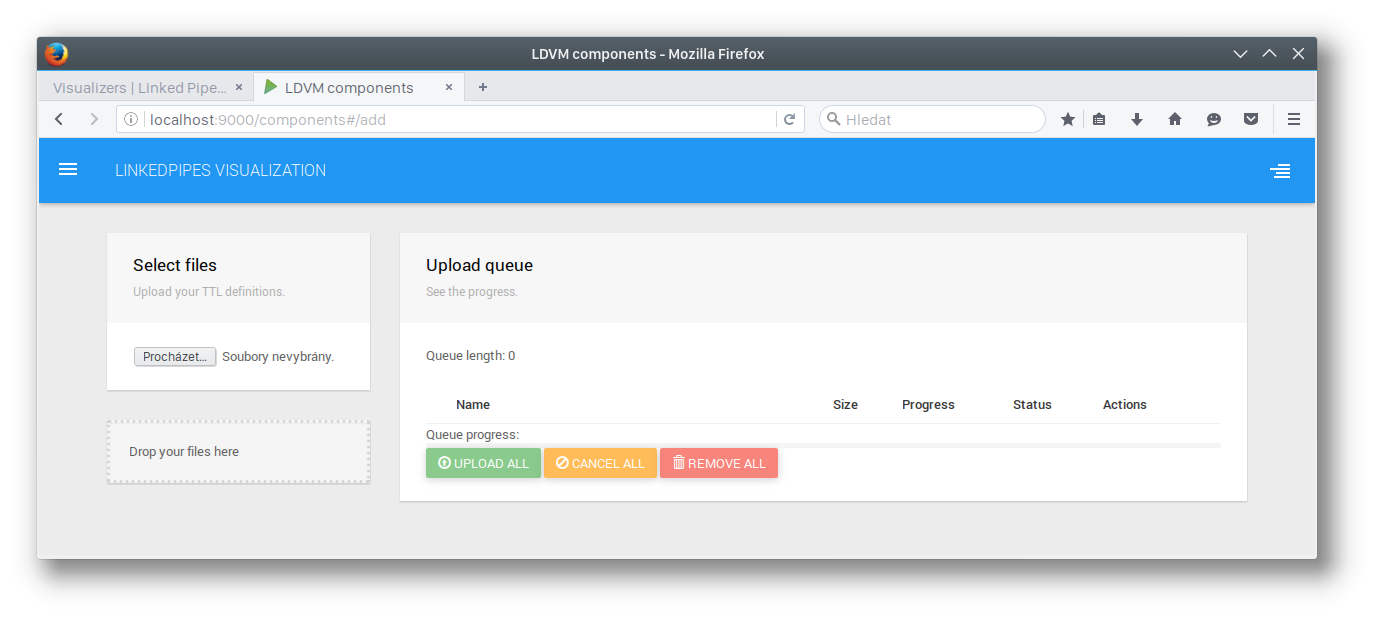
\includegraphics[width=145mm]{img/05_upload_component_definition.png}
	\caption{LinkedPipes Visualization: Upload component definition}
    \label{fig:upload_component_definition}
\end{figure}

Once this is done, the \emph{discovery} algorithm is able to utilize this new \emph{visualizer component} when discovering pipelines. If you now ran the \emph{discovery} inside LinkedPipes Visualization on a data set containing some graph data, it should find a \emph{pipeline} ending with this \emph{visualizer component}. Now we need to implement the corresponding \emph{visualizer plugin} for our \emph{application generator}.

\subsection{Frontend module}

As the first thing, we need to choose a unique short name for our \emph{visualizer}. When creating the RDF definition, we used the name \texttt{graph} as a RDF prefix. We will stick to this name.

A \emph{visualizer} has its own module in the \texttt{javascripts/modules/visualizers} folder. So we start by creating the appropriate module folder called \texttt{graph} and putting the file \texttt{prefix.js} into it.

\begin{verbatim}
import createPrefixer from '../../../misc/createPrefixer'

export const MODULE_PREFIX = 'graph';
export default createPrefixer(MODULE_PREFIX);
\end{verbatim}

As explained before, we will use the module name as a prefix for all our Redux \emph{actions} (or rather the prefix and the module name will be used as the \emph{visualizer} name). In this case, the prefix will also become part of the \emph{configurator} URL. Note that this is the actual and the only one \emph{source of truth} for the \emph{visualizer} name. The \texttt{MODULE\_PREFIX} value will be used when registering the plugin to the \emph{application generator}.

From now on, all paths will be relative to the \emph{visualizer} module (located at \texttt{javascripts/modules/visualizers/graph}).

\subsection{Configurator user interface}
\label{sec:implementation:integrating-visualizer:configurator}

The \emph{configurator} interfaces are part of the main \emph{platform} bundle. That means that while configuring his applications, the user never leaves the \emph{platform} SPA and the transitions between screens are always very smooth as complete page reloads are not necessary.

The integration is implemented through the router. The \emph{configurator} interface of every \emph{visualizer} defines its own routes that are registered to the \emph{platform} routes. Let us start with the main \texttt{Configurator} component defined in \texttt{pages/Configurator.js}.

\begin{verbatim}
import React, { Component, PropTypes } from 'react'

class Configurator extends Component {
  render() {
    return (
      <p>This is the graph visualizer configurator.</p>
    )
  }
}
export default Configurator;
\end{verbatim}

Now we create the routes file (\texttt{configuratorRoutes.js}) with the following content:

\begin{verbatim}
import React from 'react'
import { Route } from 'react-router'
import Configurator from './pages/Configurator'
import { MODULE_PREFIX } from './prefix'

export default function createRoutes(dispatch) {
  return (
    <Route component={Configurator} path={MODULE_PREFIX} />
  );
}
\end{verbatim}

Note that we used the \texttt{MODULE\_PREFIX} as the route path.

In the final step, we register our routes. That is done in \texttt{../routes.js} (one level higher, in the parent \texttt{visualizers} module). First we have to import the routes in the file header.

\begin{verbatim}
import graphRoutes from './graph/configuratorRoutes'
\end{verbatim}

Then we need to find the right place in the file and add our routes there. The spot is clearly marked with \texttt{***Here*** you register all visualizer configurator routes} and contains a list of currently registered \emph{configurator} routes. We just need to add another line for our \texttt{graph} visualizer.

\begin{verbatim}
// ***Here*** you register all visualizer configurator routes

routeFactory.register(dataCubeRoutes);
routeFactory.register(googleMapsRoutes);
routeFactory.register(chordRoutes);
routeFactory.register(graphRoutes); // We added this line
\end{verbatim}

That is it. The last remaining step is to link the LDVM \emph{visualizer component} to this module but we will do that later. An actual URL pointing to this \emph{configurator}  could look like this: \texttt{/appgen/app/8/graph}. The number \texttt{8} is the application ID that is being configured (e.g. if the user selects this application for configuration, he is redirected to this URL). In case the \emph{visualizer} name in the URL does not correspond to the selected application (for example when the user forces a different value to the URL), the user is automatically redirected to the correct \emph{configurator}.

If the reader is asking why the \emph{configurator} is part of the URL when this information can be derived directly from the application ID, we would kindly refer to Subsection \ref{sec:implementation:design-choices:integration}.

Before moving to the next step, we will slightly improve the \texttt{Configurator} component.

\begin{verbatim}
import React, { Component, PropTypes } from 'react'
import BodyPadding from '../../../../components/BodyPadding'
import { Application } from '../../../app/models'
import { Visualizer } from '../../../core/models'

class Configurator extends Component {
  static propTypes = {
    application: PropTypes.instanceOf(Application).isRequired,
    visualizer: PropTypes.instanceOf(Visualizer).isRequired
  };

  render() {
    const { application, visualizer } = this.props;
    return (
      <BodyPadding>
        <p>This is the graph visualizer configurator.</p>
        <p>{application.name}</p>
        <p>{visualizer.title}</p>
      </BodyPadding>
    )
  }
}

export default Configurator;
\end{verbatim}

The objects representing the selected application and visualizer are  for your convenience automatically injected using \texttt{props} to the \texttt{Configurator} component (but they are available from the \emph{state} at any time). Here we just use them to print their names. We also used the \texttt{BodyPadding} component to add the standard padding around the text.

\subsection{Application user interface}

As explained, the \emph{application} interface of each \emph{visualizer} lives in a standalone JavaScript bundle. The \emph{application} interface that we are about to implement will support embedding. It will run in two different modes. There will be the default \emph{standalone} mode which besides the visualization itself will also display the application name and description. It will be accessible on the default root \texttt{/} URL. Then there will be the \emph{embed} mode containing just the visualization. It will be accessible on the \texttt{/embed} URL.

We will start similarly to the \emph{configuration} interface by defining the main \texttt{Application} component in \texttt{components/Application.js}. Note that it is no longer in the \texttt{pages} folder.

\begin{verbatim}
import React, { Component, PropTypes } from 'react'
import BodyPadding from '../../../../components/BodyPadding'
import { Application as ApplicationModel } from '../../../app/models'
import { Visualizer } from '../../../core/models'

class Application extends Component {
  static propTypes = {
    application: PropTypes.instanceOf(ApplicationModel).isRequired,
    visualizer: PropTypes.instanceOf(Visualizer).isRequired,
    embed: PropTypes.bool
  };

  render() {
    const { application, visualizer, embed } = this.props;
    return (
      <BodyPadding>
        <p>This is the graph visualizer application.</p>
        <p>It runs in {embed ? 'embed' : 'standalone'} mode</p>
        <p>{application.name}</p>
        <p>{visualizer.title}</p>
      </BodyPadding>
    )
  }
}

export default Application;
\end{verbatim}

The content is at this moment almost identical to the \texttt{Configurator} component. It just displays the current application name and visualizer title. But this time it also shows whether it runs in the \emph{standalone} or \emph{embed} mode. 

Now for each mode we will need a different component as each mode lives at a different URL. Let us start with \texttt{pages/Embed.js}.

\begin{verbatim}
import React from 'react'
import Application from '../components/Application'

export default props => <Application embed {...props} />
\end{verbatim}

And now \texttt{pages/Standalone.js}.

\begin{verbatim}
import React, { PropTypes } from 'react'
import Application from '../components/Application'
import ApplicationHeader from '../../../app/components/ApplicationHeader'

const Standalone = props => (
  <div>
    <ApplicationHeader {...props} />
    <Application {...props} />
  </div>
);

export default Standalone;
\end{verbatim}

Note that both times, we re-use the \texttt{Application} component but in the \emph{standalone} mode we add a standard header that renders the application name and description. What remains is to tie it all together with routes definition. We put it to \texttt{applicationRoutes.js} just next to \texttt{configuratorRoutes.js}.

\begin{verbatim}
import React from 'react'
import { Route, IndexRoute } from 'react-router'
import ApplicationLoader from '../../app/pages/ApplicationLoader'
import NotFound from '../../platform/pages/NotFound'
import Standalone from './pages/Standalone'
import Embed from './pages/Embed'

export default function createRoutes(dispatch) {
  return (
    <Route component={ApplicationLoader} path='/'>
      <IndexRoute component={Standalone} />
      <Route component={Embed} path='embed' />
      <Route component={NotFound} path='*' />
    </Route>
  );
}
\end{verbatim}

Note that the top level path is directly \texttt{/}. This routes definition will not be registered to any existing route hierarchy. It contains the complete routing information for this standalone SPA. For this reason, we use the \texttt{ApplicationLoader} as the top level component to load the application from the server first. This has been done automatically for us in the case of \emph{configurator} interface.
 
In the final step, we need to add a new Webpack \emph{entry point}. We create a file \texttt{javascripts/entries/graph.js} (this time relative to the \texttt{assets} folder) with the following content. 

\begin{verbatim}
import createRoutes from '../modules/visualizers/graph/applicationRoutes'
import initEntry from '../misc/initEntry'

initEntry(createRoutes);
\end{verbatim}

We have to make sure to import the correct routes definition and also that the file name corresponds to the \emph{visualizer} name. Webpack will pick up this new \emph{entry point} automatically (if you are running Webpack in the watch mode, you need to restart it) and generate a new JavaScript bundle of the same name.

\subsection{Linking LDVM component to the plugin}

In this step, we will link the LDVM \emph{visualizer component} and the \emph{visualizer} plugin together. That is done through the \emph{application generator} user interface (not LinkedPipes Visualization interface this time).

We need to sign in to the \emph{application generator} with an administrator account. We navigate to the \textbf{Dashboard}, select \textbf{Visualizers} and click the button \textbf{Add visualizer}. A dialog window will appear, containing a list of unused available LDVM \emph{visualizer components}. We select \textbf{Graph Visualizer} (which is the name we provided in the RDF definition)  and click \textbf{Add visualizer}. The new \emph{visualizer} should appear in the table. We click its name to open a configuration dialog window (Figure \ref{fig:edit-visualizer}). We ignore the first two fields as they are related to LinkedPipes Visualization. The most important field is the name. We fill in \texttt{graph}. It is crucial that this value corresponds to the \emph{visualizer} module name, the prefix and the \emph{entry point} name. We also recommend filling in the \emph{visualizer} icon for better user experience. Currently, Material Icons \footnote{https://design.google.com/icons/} collection is used. We chose the \texttt{device\_hub} icon.

\begin{figure}
	\centering
	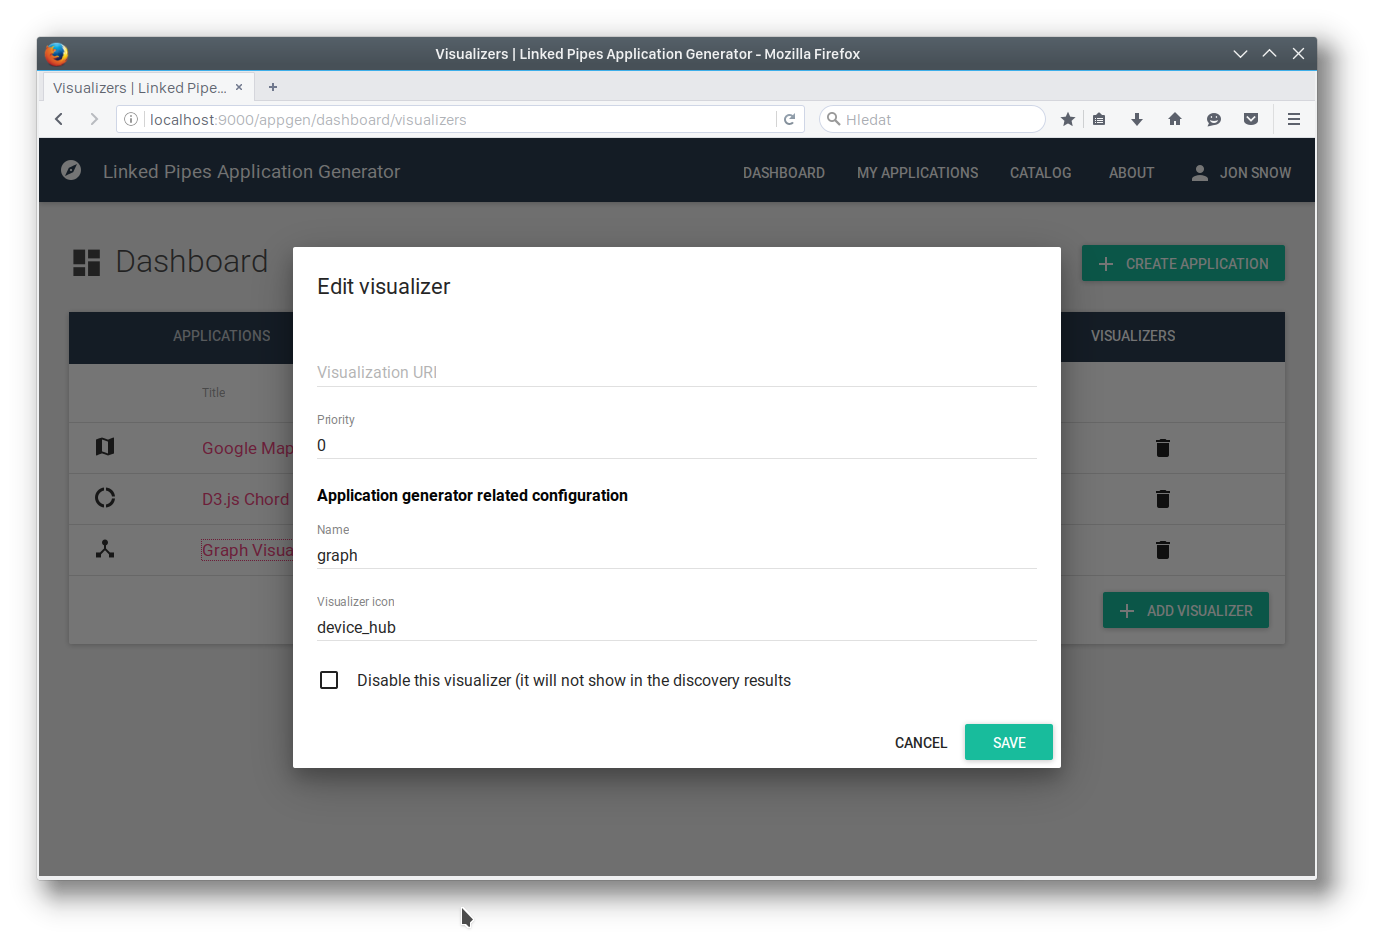
\includegraphics[width=140mm]{img/05_edit_visualizer.png}
	\caption{Configuration dialog window of a \emph{visualizer}.} 
	\label{fig:edit-visualizer}
\end{figure}
This was the last mandatory step. At this moment, the \emph{visualizer} (even though it does not do anything) should be working, i.e., it should be possible to create a new application using this \emph{visualizer} from a data set containing graph data.

\subsection{Scala backend}

Surprisingly enough, we did not have to touch the Scala backend to register our new \emph{visualizer}. Technically speaking, it is really not necessary but only until the very moment when we need the \emph{visualizer} to actually \textit{do something useful}. That typically involves fetching and extracting the RDF data produced by the \emph{pipeline}. For that we do need the backend.

In this subsection, we will simply prepare the controller that will be handling our client requests.

\begin{verbatim}
package controllers.appgen.api.visualizers
import scaldi.Injector

class GraphVisualizerApiController(implicit inj: Injector) extends VisualizerApiController { }
\end{verbatim}

The package information clearly says where this class should belong. The \texttt{VisualizerApiController} will provide us with some utilities that will come handy later.

\subsection{Extracting RDF data from the pipeline evaluation}
\label{sec:implementation:integrating-visualizer:extracting-rdf}

We said that our \emph{visualizer} would show the number of vertices and edges in the graph. For us that means that we need to access the RDF data produced by the \emph{pipeline}, extract this information from it, send it to the client and then display it on the screen. We start with accessing the RDF data.

Since it is RDF data, we will use SPARQL queries to fetch the information we need. 

\begin{verbatim}
package model.rdf.sparql.rgml.query
import model.rdf.sparql.query.SparqlQuery

class GraphQuery extends SparqlQuery {

  def get: String =
    """
      | PREFIX rdf: <http://www.w3.org/1999/02/22-rdf-syntax-ns#>
      | PREFIX rgml: <http://purl.org/puninj/2001/05/rgml-schema#>
      |
      | SELECT ?directed ?nodeCount ?edgeCount WHERE {
      |   ?graph
      |     rdf:type rgml:Graph ;
      |     rgml:directed ?directed .
      |
      |   { SELECT (COUNT(*) AS ?nodeCount) WHERE { ?edge rdf:type rgml:Node . } }
      |   { SELECT (COUNT(*) AS ?edgeCount) WHERE { ?edge rdf:type rgml:Edge . } }
      | }
      | LIMIT 1
    """
      .stripMargin
}
\end{verbatim}

This is the recommended way of representing SPARQL queries in our Scala code. As you can see, the query counts all the edges and vertices (which are called \emph{nodes} in the RGML vocabulary) and also fetches the information about whether the graph is directed or not.

The result of this query will be represented using a simple Scala case class. For simplicity, we just call it \texttt{Graph}.

\begin{verbatim}
package model.rdf.sparql.rgml

case class Graph(directed: Boolean, nodeCount: Int, edgeCount: Int)
\end{verbatim}

Now we need a tool that will convert the fetched RDF data into this case class. Such a tool is called an \emph{extractor}.

\begin{verbatim}
package model.rdf.sparql.rgml.extractor

import model.rdf.extractor.QueryExecutionResultExtractor
import model.rdf.sparql.rgml.Graph
import model.rdf.sparql.rgml.query.GraphQuery
import org.apache.jena.query.QueryExecution


class GraphExtractor extends QueryExecutionResultExtractor[GraphQuery, Graph] {

  def extract(input: QueryExecution): Option[Graph] = {

    try {
      val resultSet = input.execSelect()

      if (!resultSet.hasNext) return None

      val solution = resultSet.nextSolution()
      Some(Graph(
        solution.getLiteral("directed").getBoolean,
        solution.getLiteral("nodeCount").getInt,
        solution.getLiteral("edgeCount").getInt))
    } catch {
      case e: org.apache.jena.sparql.engine.http.QueryExceptionHTTP => {
        None
      }
    }
  }
}
\end{verbatim}

Apache Jena \footnote{https://jena.apache.org/} framework is used internally to work with RDF data. Our SPARQL query is a SELECT query which means that the results will be in a form of tabular data (i.e., a set of rows where each row contains the same columns). We assume that the data set contains only one graph, so we take the first row (if available) and convert it to the \texttt{Graph} case class.

Finally, we need something that will execute the query and apply the extractor on the results.

\begin{verbatim}
package model.rdf.sparql.rgml
//  ...imports

class RgmlService(implicit val inj: Injector) extends RgmlService with Injectable {
  var sparqlEndpointService = inject[SparqlEndpointService]

  def graph(evaluation: PipelineEvaluation)(implicit session: Session): Option[Graph] = {
    sparqlEndpointService.getResult(
      evaluationToSparqlEndpoint(evaluation),
      new GraphQuery(),
      new GraphExtractor())
  }
\end{verbatim}

As you can see, we defined \texttt{RgmlService} with the \texttt{graph} method. The \emph{pipeline evaluation} does not directly contain the data but rather points where the data are (i.e., it specifies the SPARQL endpoint and concrete named graphs with the data). We use \texttt{SparqlEndpointService} to access it and extract our graph from it. The function \texttt{evaluationToSparqlEndpoint} is just an utility that we omitted to keep the code short. % TODO: add it to a trait

You might have noticed that we put all the files in the same package \texttt{model.rdf.sparql.rgml}. What we are doing is that we are adding support for RGML vocabulary to the LinkedPipes Visualization code base in a way that anyone can use it for their \emph{visualizers}, i.e., it is \emph{visualizer} independent.

For the \texttt{RgmlService} to work properly, it has to be registered to the Dependency Injection container in \texttt{model.rdf.RdfModule}.

Let us now move from the \emph{Model} layer to the \emph{Controller} layer. We will extend the controller we defined earlier with an action that will use this service to fetch the graph information and send it to the client serialized to JSON.

\begin{verbatim}
class GraphVisualizerApiController(implicit inj: Injector) extends VisualizerApiController {
  val rgmlService = inject[RgmlService]

  def getGraph(id: Long) = RestAsyncAction[EmptyRequest] { implicit request => json =>
    withEvaluation(ApplicationId(id)) { evaluation =>
      val graph = rgmlService.graph(evaluation)
      Future(Ok(SuccessResponse(data = Seq("graph" -> graph))))
    }
  }
}
\end{verbatim}

The \texttt{getGraph} action is mapped to a URL with a single parameter \texttt{id} (the URL mappings are defined in the file \texttt{src/conf/routes}, relative to the code base root). The \texttt{id} is an application ID. We use the \texttt{withEvaluation()} helper to load the appropriate \emph{pipeline evaluation}, then we fetch the graph using our \texttt{RgmlService} and send it to the client in a \texttt{SuccessReponse}. The API is designed to support \texttt{Futures} in case the requests are expected to be computationally heavy and need to be performed asynchronously. This is not our case but we need to follow the API. That is why the response is wrapped by the \texttt{Future} call.

In order for the \texttt{Graph} case class to be automatically converted to JSON, we need to define an \emph{implicit converter}. We can do it by adding following lines to \texttt{controllers.api.JsonImplicits} and import it to the controller:

\begin{verbatim}
implicit val graphWrites = Json.writes[Graph]
\end{verbatim}

\subsection{Making asynchronous requests from the client}

Everything is prepared on the server-side. Now comes the client. When the application loads, we will make an synchronous HTTP request to fetch the graph information. Once we receive it, we store it in the \emph{state} and show it on the screen.

We start by creating a JavaScript counterpart for the Scala \texttt{Graph} case class. Note that once again, all paths are relative to the \emph{visualizer} module. Also to keep the text shorter, we will just state the file name at the beginning of each snippet.

\begin{verbatim}
// models.js

import { Record } from 'immutable';

export const Graph = Record({
  directed: false,
  nodeCount: 0,
  edgeCount: 0
});
\end{verbatim}

We create a simple explicit wrapper for the asynchronous HTTP request.

\begin{verbatim}
// api.js

import rest from '../../../misc/rest'

export async function getGraph(applicationId) {
  const result = await rest('graphVisualizer/getGraph/' + applicationId, {});
  return result.data.graph;
}
\end{verbatim}

The keywords \texttt{async/await} are just syntactical sugar around \texttt{Promises}. They allow us to write \emph{asynchronous} code in a \emph{synchronous} manner.

Now we will define a new \emph{duck} that will handle and provide API for fetching the graph information (using an \emph{action}), storing it in the \emph{state} (using a \emph{reducer}) and selecting it from the \emph{state} (using a \emph{selector}). Let us start with \emph{actions} (we will always put the currently required \texttt{imports} to the top of each code snippet; in the actual file they will all be together at the beginning).

\begin{verbatim}
// ducks/graph.js

import createAction from '../../../../misc/createAction'
import withApplicationId from '../../../app/misc/withApplicationId'
import prefix from '../prefix'
import * as api from '../api'

// Actions

export const GET_GRAPH = prefix('GET_GRAPH');
export const GET_GRAPH_START = GET_GRAPH + '_START';
export const GET_GRAPH_ERROR = GET_GRAPH + '_ERROR';
export const GET_GRAPH_SUCCESS = GET_GRAPH + '_SUCCESS';
export const GET_GRAPH_RESET = GET_GRAPH + '_RESET';

export function getGraph() {
  return withApplicationId(id => {
    const promise = api.getGraph(id);
    return createAction(GET_GRAPH, { promise });
  })
}

export function getGraphReset() {
  return createAction(GET_GRAPH_RESET);
}
\end{verbatim}

The \emph{action creator} \texttt{getGraph()} first uses the \texttt{withApplicationId} utility to extract the application ID from the \emph{state} and then calls the API function to make the HTTP request to the server. The request result is represented using a \texttt{Promise} which is \emph{dispatched} as an action payload. There is a \emph{redux middleware} running in the background that detects the \texttt{Promise}, dispatches \texttt{GET\_GRAPH\_START} and then depending on the result either \texttt{GET\_GRAPH\_ERROR} or \texttt{GET\_GRAPH\_SUCCESS}. We do not actually have to define all the \emph{action} constants but it is good practice (note that we used the module prefixer). The \texttt{START}, \texttt{ERROR}, \texttt{SUCCESS} and \texttt{RESET} suffixes are defined by a convention.

In the next step, we will implement the reducer that will store the graph.

\begin{verbatim}
// ducks/graph.js

import { GET_APPLICATION_START } from '../../../app/ducks/application'
import { Graph } from '../models'

// Reducer

const initialState = new Graph();

export default function graphReducer(state = initialState, action) {
  switch (action.type) {
    case GET_APPLICATION_START:
    case GET_GRAPH_RESET:
      return initialState;

    case GET_GRAPH_SUCCESS:
      return new Graph(action.payload);
  }

  return state;
};
\end{verbatim}

Note that the initial state is a valid (but empty) \texttt{Graph} object. That means that we can work with this object safely at any time (it will not be \texttt{null}).

Finally, we will create \emph{selectors} that will allow us to easily extract the \texttt{Graph} from the state.

\begin{verbatim}
// ducks/graph.js

import { createSelector } from 'reselect'
import { createPromiseStatusSelector } from '../../../core/ducks/promises'
import moduleSelector from '../selector'

// Selectors

export const graphStatusSelector = createPromiseStatusSelector(GET_GRAPH);
export const graphSelector = createSelector([moduleSelector], state => state.graph);
\end{verbatim}

The first one selects the HTTP request status, the second one selects the actual graph. Now we need to integrate both the \emph{selectors} and the \emph{reducer} to the \emph{state} hierarchy.

\begin{verbatim}
// reducer.js

import { combineReducers } from 'redux';
import graph from './ducks/graph'

const rootReducer = combineReducers({
  graph
});

export default rootReducer;
\end{verbatim}

This is the root \emph{reducer} of the \emph{visualizer} module that combines all other reducers in the module together. It has to be registered to the parent reducer in the parent module.

\begin{verbatim}
import { combineReducers } from 'redux';
import googleMaps from './googleMaps/reducer'
import chord from './chord/reducer'
import graph from './graph/reducer'

const rootReducer = combineReducers({
  googleMaps,
  chord,
  graph // We added this line
});
export default rootReducer;
\end{verbatim}

We have to do the same for the \emph{selectors} as well.

\begin{verbatim}
// selector.js

import { createSelector } from 'reselect'
import parentSelector from '../selector'
import { MODULE_PREFIX } from './prefix'

export const moduleSelector = createSelector(
  [parentSelector],
  parentState => parentState[MODULE_PREFIX]
);
export default moduleSelector;
\end{verbatim}

You might have noticed that we already used this file in \texttt{ducks/graph.js}. What is important here is that the key we use to register the \emph{reducer} is the same as the key we use in the \emph{selector}. They both access the same data in the same \emph{state} object (\emph{reducer} for updating, \emph{selector} for reading).

Now that everything is ready, we create a simple component that will fetch and display the graph information. We start with the component life cycle methods.

\begin{verbatim}
// components/GraphLoader.js

import React, { Component, PropTypes } from 'react'
import { getGraph, getGraphReset } from '../ducks/graph'

class GraphLoader extends Component {
  componentWillMount() {
    const { dispatch } = this.props;
    dispatch(getGraph());
  }
  
  componentWillUnmount() {
    const { dispatch } = this.props;
    dispatch(getGraphReset());
  }
}
\end{verbatim}

Once the component appears on the screen, it will initiate the request. When it is about to leave, it will reset the \emph{state} 
(clean up after itself). We will \emph{connect} the component to Redux and inject the data that we need.

\begin{verbatim}
// components/GraphLoader.js

import { connect } from 'react-redux'
import { createStructuredSelector } from 'reselect'
import { getGraph, getGraphReset, graphSelector, graphStatusSelector } from '../ducks/graph'

const selector = createStructuredSelector({
  graph: graphSelector,
  status: graphStatusSelector
});

export default connect(selector)(GraphLoader);
\end{verbatim}

It is always a good practice to explicitly define the \texttt{propTypes}.

\begin{verbatim}
// components/GraphLoader.js

import { PromiseStatus } from '../../../core/models'
import { Graph } from '../models'

class GraphLoader extends Component {
  static propTypes = {
    dispatch: PropTypes.func.isRequired,
    graph: PropTypes.instanceOf(Graph).isRequired,
    status: PropTypes.instanceOf(PromiseStatus).isRequired
  };
  
  // ...
}
\end{verbatim}

Lastly, we implement the \texttt{render} method.

\begin{verbatim}
// components/GraphLoader.js

import PromiseResult from '../../../core/components/PromiseResult'

class GraphLoader extends Component {
  // ...
  
  render() {
    const { graph, status } = this.props;

    if (!status.done) {
      return <PromiseResult status={status} loadingMessage="Loading base graph info..." />
    }

    return (
      <div>
        <p><strong>Graph info</strong></p>
        <p>Node count: {graph.nodeCount}</p>
        <p>Edge count: {graph.edgeCount}</p>
        <p>Directed: {graph.directed ? 'yes' : 'no'}</p>
      </div>
    )
  }
\end{verbatim}

The \texttt{status.done} value changes to \texttt{true} only if the request successfully finishes (i.e., the \emph{action} \texttt{GET\_GRAPH\_SUCCESS} is \emph{dispatched}). Therefore once the value is \texttt{true} we can be sure that the graph information is correctly stored in the \emph{state}. Before this happens, we display the \texttt{PromiseResult} component which shows a nice loading bar and if the request fails, it displays an error message. 

What remains to be done is to add the \texttt{GraphLoader} component to the \emph{configurator} and \emph{application} user interface.

\begin{verbatim}
// pages/Configurator.js

import GraphLoader from '../containers/GraphLoader'

class Configurator extends Component {
  // ...

  render() {
    const { application, visualizer } = this.props;
    return (
      <BodyPadding>
        <p>This is the graph visualizer configurator.</p>
        <p>{application.name}</p>
        <p>{visualizer.title}</p>
        <GraphLoader />
      </BodyPadding>
    )
  }
}
\end{verbatim}

\begin{verbatim}
// components/Application.js

import GraphLoader from '../containers/GraphLoader'

class Application extends Component {
  // ...

  render() {
    const { application, visualizer, embed } = this.props;
    return (
      <BodyPadding>
        <p>This is the graph visualizer application.</p>
        <p>It runs in {embed ? 'embed' : 'standalone'} mode</p>
        <p>{application.name}</p>
        <p>{visualizer.title}</p>
        <GraphLoader />
      </BodyPadding>
    )
  }
}
\end{verbatim}

\subsection{Saving and loading application configuration}
\label{sec:implementation:integration:configuration}

The framework provides an optional solution for saving and loading the application configuration easily. The idea is very simple, the configuration consists of different bits and pieces of the \emph{state}. To save the configuration, we just serialize those bits and pieces into JSON and save it on the server. To load the configuration, we fetch it from the server, unserialize it from JSON and let the \emph{reducers} to update the \emph{state}.

The configuration contains parts that are \emph{visualizer} specific and parts that are common for all \emph{visualizers} and we have to make sure that they both are saved and loaded properly together.

We starting by creating a \texttt{dirty} \emph{duck} with a \emph{reducer} that will simply indicate with a boolean value whether the configuration has changed.

\begin{verbatim}
// ducks/dirty.js

import { createSelector } from 'reselect'
import moduleSelector from '../selector'
import { createDirtyReducer } from '../../../app/ducks/dirty'

// Reducer

const actions = [ ];

export default createDirtyReducer(actions);

// Selectors

export const dirtySelector = createSelector([moduleSelector], state => state.dirty);
\end{verbatim}

The \texttt{actions} constant contains the list of \emph{actions} that change the state. Whenever such an \emph{action} is dispatched, the \emph{dirty} status changes to \texttt{true}. The \emph{reducer} has to be properly registered in the module root \emph{reducer}.

The next \emph{duck} will define the \emph{actions} for saving and loading the configuration. They will be created using framework factories that will ensure proper integration.

\begin{verbatim}
import prefix from '../prefix'
import moduleSelector from '../selector'
import { createPromiseStatusSelector } from '../../../core/ducks/promises'
import { 
  createGetConfiguration, createGetConfigurationReset, createSaveConfiguration 
} from '../../../app/ducks/configuration'

// Actions

export const SAVE_CONFIGURATION = prefix('SAVE_CONFIGURATION');
export const SAVE_CONFIGURATION_START = SAVE_CONFIGURATION + '_START';
export const SAVE_CONFIGURATION_ERROR = SAVE_CONFIGURATION + '_ERROR';
export const SAVE_CONFIGURATION_SUCCESS = SAVE_CONFIGURATION + '_SUCCESS';

export const GET_CONFIGURATION = prefix('GET_CONFIGURATION');
export const GET_CONFIGURATION_START = GET_CONFIGURATION + '_START';
export const GET_CONFIGURATION_ERROR = GET_CONFIGURATION + '_ERROR';
export const GET_CONFIGURATION_SUCCESS = GET_CONFIGURATION + '_SUCCESS';
export const GET_CONFIGURATION_RESET = GET_CONFIGURATION + '_RESET';

// Selectors

export const saveConfigurationStatusSelector = createPromiseStatusSelector(SAVE_CONFIGURATION);
export const getConfigurationStatusSelector = createPromiseStatusSelector(GET_CONFIGURATION);

export const configurationSelector = createSelector(
  [moduleSelector],
  state => ({  })
);

// Actual actions created using factories
export const saveConfiguration = 
  createSaveConfiguration(SAVE_CONFIGURATION, configurationSelector);
export const getConfiguration = 
  createGetConfiguration(GET_CONFIGURATION);
export const getConfigurationReset = 
  createGetConfigurationReset(GET_CONFIGURATION_RESET);
\end{verbatim}

The \texttt{configurationSelector} defines what parts of the \emph{state} should get into the configuration. At this moment, the \emph{state} just contains the graph information which is available from the \emph{pipeline evaluation}. There is no point in making that part of the configuration. When the configuration is loaded from the server, the \emph{action} \texttt{GET\_CONFIGURATION\_SUCCESS} is \emph{dispatched} with the configuration in the payload. The \emph{reducers} can simply listen to this action and extract from the payload the information that is relevant to them. As the \emph{action} is prefixed, it will not cause any conflicts.

The next step of integration is the \textbf{Save} button. Once again we use a framework factory to create the button component. The button is interactive which means it automatically indicates whether the configuration needs to be saved (using the \texttt{dirty} information) or whether the saving is in progress. We will add the button to the \texttt{Configurator} component.

\begin{verbatim}
import React, { PropTypes } from 'react'
import { saveConfiguration, saveConfigurationStatusSelector } from '../ducks/configuration'
import { dirtySelector } from '../ducks/dirty'

import createSaveButton from '../../../app/containers/createSaveButton'

export default createSaveButton(
  saveConfiguration,
  saveConfigurationStatusSelector,
  dirtySelector);
\end{verbatim}

In the final step, we need to load the configuration when the \emph{configurator} (or \emph{application}) initiates.

\begin{verbatim}
// pages/Configurator.js

import { getConfiguration, getConfigurationReset } from '../ducks/configuration'

class Configurator extends Component {
  // ...

  componentWillMount() {
    const { dispatch } = this.props;
    dispatch(getConfiguration());
  }

  componentWillUnmount() {
    const { dispatch } = this.props;
    dispatch(getConfigurationReset());
  }
  
  // ...
}
\end{verbatim}

Similarly, we would load the configuration in the \texttt{Application} component.

As a concrete example, we will let the user to edit graph label. To keep this subsection short, we will utilize one of the available framework utilities, custom label editor. This editor allows the user to specify alternative labels for RDF resources. Each RDF resource is identified with a URI. Unfortunately, we do not have the graph URI but for simplicity, we will just make up one.

\begin{verbatim}
// pages/Configurator.js

import EditableLabel from '../../../app/containers/EditableLabel'
import SaveButton from '../containers/SaveButton'

class Configurator extends Component {
  // ...

  render() {
    const { application, visualizer } = this.props;
    return (
      <BodyPadding>
        <h3><EditableLabel uri="http://example.org/graph" label="Unnamed graph" /></h3>
        <p>This is the graph visualizer configurator.</p>
        <p>{application.name}</p>
        <p>{visualizer.title}</p>
        <GraphLoader />
        <SaveButton />
      </BodyPadding>
    )
  }
}
\end{verbatim}

That is it. If we now click the \textbf{More} button in the upper right corner of the \emph{configurator} interface and then select \textbf{Edit labels}, a pencil icon will appear next to the graph name (which will be "Unnamed graph" by default). Clicking that icon will open a dialog where we can define a language dependent values for this resource. By clicking \textbf{Save}, we update the \emph{state} and we can immediately see the change on the screen. By clicking \textbf{Save changes}, we save the changes to the server (the custom labels are part of the common configuration which means that it is automatically taken care of). We now have to add the \texttt{EditableLabel} component to the \texttt{Application} component as well to get it working in the \emph{application} interface.

You might have noticed that we have repeated a lot of work for the \emph{application} and \emph{configurator} interface and their components are nearly identical. Firstly, in a more complex \emph{visualizer} those two interfaces would differ significantly more. Secondly, thanks to the React nature it is always very easy to refactor the code, put the shared aspects into a single component and then re-use it.

The result of our work can be seen on Figure \ref{fig:graph-visualizer}. For more complex examples we suggest the user to check out the full implementations of the two completed visualizers, the D3.js Chord Visualizer and Google Maps Visualizer (both will be explained later).

\begin{figure}
	\centering
	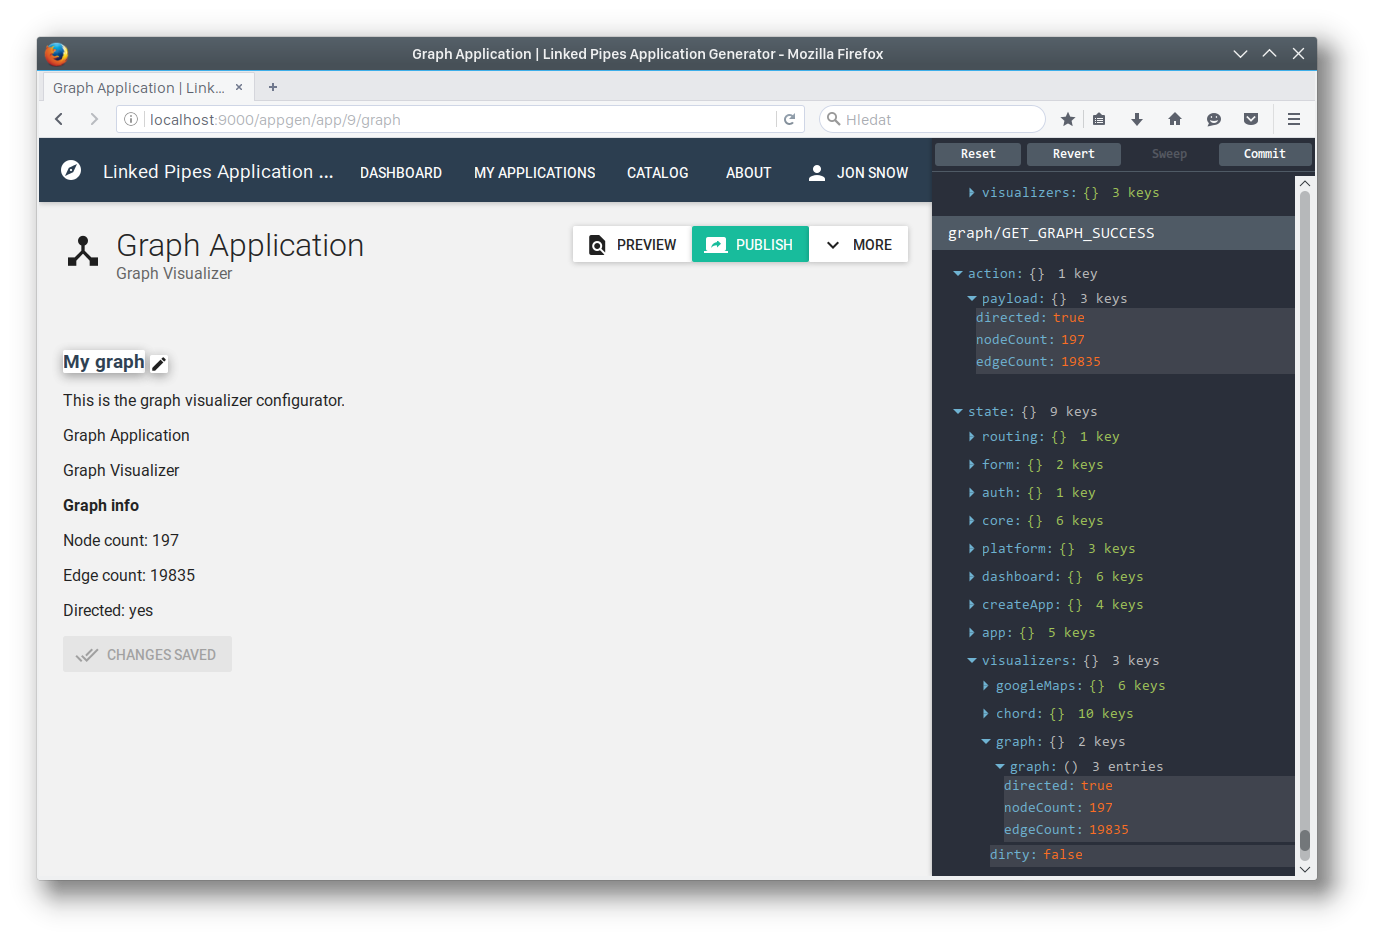
\includegraphics[width=145mm]{img/05_graph_visualizer}
	\caption{\emph{Configurator} interface of the sample Graph Visualizer. The Redux development sidebar is enabled showing the \emph{state}.}
    \label{fig:graph-visualizer}
\end{figure}

\section{Advanced framework features}

While we were demonstrating how a new \emph{visualizer} can be integrated into our \emph{application generator}, we showed couple of available features that the developer can use to speed up the process. Namely, we described the prepared solution for saving and loading application configuration and we also showed how we can easily extract RDF data from the \emph{pipeline evaluation}. Here we will briefly mention couple more examples.

\subsection{Request cache}

As some requests might be quite computationally heavy, we implemented a simple caching solution for the server side. For example, this is the controller action that fetches the graph information (Subsection \ref{sec:implementation:integrating-visualizer:extracting-rdf}):

\begin{verbatim}
class GraphVisualizerApiController(implicit inj: Injector) extends VisualizerApiController {
  val rgmlService = inject[RgmlService]

  def getGraph(id: Long) = RestAsyncAction[EmptyRequest] { implicit request => json =>
    withEvaluation(ApplicationId(id)) { evaluation =>
      val graph = rgmlService.graph(evaluation)
      Future(Ok(SuccessResponse(data = Seq("graph" -> graph))))
    }
  }
}
\end{verbatim}

Making this request cached is very simple:

\begin{verbatim}
class GraphVisualizerApiController(implicit inj: Injector) extends VisualizerApiController {
  val rgmlService = inject[RgmlService]

  def getGraph(id: Long) = RestAsyncAction[EmptyRequest] { implicit request => json =>
    cached {
      withEvaluation(ApplicationId(id)) { evaluation =>
        val graph = rgmlService.graph(evaluation)
        Future(Ok(SuccessResponse(data = Seq("graph" -> graph))))
      }
    }
  }
}
\end{verbatim}

The solution works on a request level (it uses all available request information, including URL, POST data and the current user to identify the request). What is important is that the requests are cached persistently in the database which means that the cache will survive even application crashes. The solution is very basic and the point is just to demonstrate the capabilities. The default caching solution for the Play Framework is Ehcache \footnote{http://www.ehcache.org/} but that supports persistent caching only in the paid version.

\subsection{Multiple language support}

RDF may contain values (typically labels) in multiple languages. If correctly extracted, such a value is represented using the \texttt{model.rdf.LocalizedValue} Scala case class which, serialized to JSON, looks like this:

\begin{verbatim}
{
  'variants': {
    'en': 'Czech Republic',
    'cs': 'Česká republika'
  }
}
\end{verbatim}

The frontend framework offers a simple way how to display these values.

\begin{verbatim}
import React from 'react'
import LocalizedValue from './LocalizedValue'

const Country = country => (
    <h3><LocalizedValue localizedValue={country.label} /></h3>
  );
\end{verbatim}

If the \texttt{country.label} value is in the format suggested above, the component will automatically choose the value corresponding to the language currently selected by the user (if it is available).

The problem here is to determine what languages are actually available (i.e., what languages the user can select from). As this information is not available anywhere, we use a \emph{brute force} solution to find it. In Redux, every \emph{action} is \emph{dispatched} to every \emph{reducer}. Typically, one \emph{reducer} only responds to couple of related \emph{actions} but to solve our problem, we introduced a special \emph{reducer} that responds to every \emph{action} and searches through the payloads for available languages (it is looking for the object structure suggested above). The \emph{reducer} uses a simple Depth-first search algorithm to recursively search through the whole payload.

For example, whenever we fetch something from the server, the incoming data are \emph{dispatched} as a payload of some \texttt{SUCCESS} action. Our special \emph{reducer} searches that payload and if it finds any new languages, it adds them to the \emph{state}. An updated language switch is consequently displayed to the user.

\subsection{Label dereferencing}
\label{sec:implementation:advanced-features:label-dereferencering}

It is pretty common that an RDF resource contains a label which we can display to the user. But sometimes it is not available in frontend, maybe because it was simply not fetched from the server, maybe because it is not present in the data set at all. The frontend framework offers another useful component that attempts to fix this problem.

\begin{verbatim}
import React from 'react'
import LocalizedValue from './LocalizedValue'

const Country = country => (
    <h3><Label uri={country.uri} label={country.label} /></h3>
  );
\end{verbatim}

If \texttt{country.label} is empty, the component will make a request to the server which will at first try to load the label from the \emph{pipeline evaluation} and if the label is not there, it will use a technique called \emph{dereferencing}. That involves directly accessing the resource URI using the HTTP protocol and trying to extract the label from the response.

Note that the \texttt{Label} component wraps the \texttt{LocalizedValue} component which means that if the label supports multiple languages, the correct language variant will be displayed. Also note that the component is smart enough so even if you display 100 labels at once, only one request with 100 URIs will be sent to the server.

\subsection{Custom labels editor}

We have already explained how the custom labels editor work (Subsection \ref{sec:implementation:frontend-development-stack:redux}). Using a component \texttt{EditableLabel} you can allow the user to provide his own labels for any RDF resource. Here we would just like to say that this component internally uses the aforementioned \texttt{Label} component. That means that \texttt{EditableLabel} supports multiple languages and also if the label is missing and is not provided by the user, it is fetched from the server.

We believe this nicely shows the strength of our development stack. Each of these three components (\texttt{LocalizedValue}, \texttt{Label}, \texttt{EditableLabel}) has a single purpose and by simple composition we achieve pretty interesting results. Also the developer can drop any of these components wherever he wants and it \emph{just works}. This approach shows a lot of potential for other similar solutions.

\subsection{Miscellaneous}

The framework also contains a lot of smaller and less important features which, however, can be of great help for the developer in certain situations. Especially because  the chosen development stack lacks many features that a well-established monolithic framework would offer.  We will just provide a brief list of some of them. 

\begin{itemize}
\item \textbf{Pagination} -- correctly implementing frontend pagination is a challenge. We humbly offer our own solution.
\item \textbf{Dialog windows} -- complete solution for managing dialog windows using the Redux \emph{state}.
\item \textbf{Notifications} -- displaying simple on-screen notifications.
\item \textbf{Promise integration} -- complete solution for asynchronous requests including on-screen feedback and dealing with errors.
\item \textbf{Material UI} \footnote{http://www.material\-ui.com/} -- integration of this UI library providing components for building rich user interfaces.

\end{itemize}
\section{Design choices regarding the framework}

In this final section of this chapter, we will share some ideas that we feel should be mentioned but are not that important to be included to the previous parts of this chapter.

\subsection{Integration of new visualizers}
\label{sec:implementation:design-choices:integration}

In Subsection \ref{sec:implementation:integrating-visualizer:configurator} we explained how a new \emph{configurator} can be integrated into the \emph{application generator}. The way the current solution works is that the particular \emph{configurator} that is used to configure an application is part of the \emph{configurator} interface URL. The reader might ask why this is necessary when this information can be derived directly from the application ID. We will try to shortly justify our decisions.

Our main goal was to allow the developer to define his own routes for the \emph{configurator} so that it can be navigated using URLs  (in the example from \ref{sec:implementation:integrating-visualizer:configurator}, the \emph{configurator} uses just a single route but that is only because we wanted to keep the example simple). In  React-router, the routes are defined in a hierarchical manner. That is perfect for our cause. The developer can create his own arbitrarily complex hierarchy of routes and simply plug it to the rest of the routes without being afraid of any conflicts.

However, what we need in this case are \emph{dynamic} routes, i.e., depending on the selected application, we would choose the appropriate route definition of the \emph{configurator} demanded by the application. As it turns out, such \emph{dynamic} routes are supported by React-router but we were not aware of that in the early phases when we were designing this mechanism. So instead we chose this solution when the routes definition is registered under the \emph{visualizer} name and we just have to make sure that the user is always redirected to the right URL.

What is important here is that this approach, despite being a bit cumbersome and illogical, does not in any way diminish the comfort of registering new \emph{configurators}. It should be possible to re-implement the mechanism to use the \emph{dynamic} routes (and therefore leave out the \emph{visualizer} name from the URL) without any API changes.

\subsection{Integration flexibility}

In Section \ref{sec:implementation:integrating-visualizer} we thoroughly described the process of integrating a new \emph{visualizer}. What has not been said is that many of those steps, even though recommended, are in fact optional.

As far as the \emph{configurator} interface is concerned, once the \texttt{Configurator} component is mounted, the developer is free to do anything he wants inside this component. As React offers API to access the underlying DOM nodes, the user can even step out of React and start using any other framework that he feels would suit his needs. It is even possible to insert an \texttt{iframe} and render the \emph{configurator} interface using the Play Framework \emph{View} layer.

The \emph{application} interface is even more flexible. Each interface is a standalone SPA and the developer has the Webpack entry point file under his full control. Therefore if he decides, he does not even have to use our development stack including React and other tools. He can instead from the very beginning use his own solution.

With this said, we have to explicitly state that we do not recommend any of this. We suggest that the developer follows the standard process as defined in Section \ref{sec:implementation:integrating-visualizer} because only then he can benefit from all the solutions that we have prepared. On the other hand, the developer might find himself in a situation when our approach is not suitable for his needs. For example, React might not be performant enough for particular visualizations or there might be a complete external solution available that the developer would like to utilize. That is why we feel it is a good thing that the developer is given such freedom even though it means that the API is not as elegant as it could be.
   
\chapter{Visualizers}

\section{D3.js Chord Visualizer}

\section{Google Maps Visualizer}



\chapter{Theoretical attachment}
\label{chap:theoretical-attachment}

In this chapter, we will describe and analyze two algorithms that we implemented when developing the D3.js Chord Visualizer (Section \ref{sec:visualizers:chord}).

\section{Calculating the graph adjacency matrix for the chord diagram}

A graph represented in RDF presented a certain challenge. In our first implementation (when we needed quick results) we would simply load the whole graph into memory, represent it using Scala native data structures and then work with this representation. This approach proved itself sufficient and actually pretty efficient for small graphs (for example the asylum seekers data set, see Subsection \ref{sec:visualizers:chord:data-sets} for data sets description). Compared to SPARQL queries (which involve 
\todo[color=green!40]{Přístupové časy do paměti, na disk a po síti se liší řádově, což předpokládám patří k základním znalostem matfyzáků. Či je i toto potřeba podložit?}
accessing the hard drive or even communication over network in case the triple store is on a separate machine), in-memory operations are way faster and fetching couple of hundreds nodes and edges in every request was bearable (we needed just two queries to fetch the nodes and the edges).

The situation changed (the performance dropped) when we started experimenting with the air routes data set, containing around 8000 airports and almost 70000 routes. To improve performance and support even bigger graphs, we decided to re-implement the service so that the complexity of any operation would depend on the size of the input, not on the size of the graph. That typically means, that we would never do operations like loading all nodes or edges into memory. Obviously, we can guarantee this assumption only in our own code. The triple store (e. g. Virtuoso) might work differently.

\subsection{Adjacency matrix}

Let us have a look at how generating the adjacency matrix for the chord diagram works. An adjacency matrix for a directed graph is a square matrix where the $(i, j)$ value indicates whether there is an edge going from the node $i$ to the node $j$. Typically this value is either $1$ (nodes are connected in this direction) or $0$ (nodes are not connected in this direction). In our case, however, the graph is a directed weighted multigraph. Such a graph is impossible to represent using this kind of adjacency matrix because we would need to distinguish somehow between having two nodes connected by $10$ edges of weight $1$ or by $1$ edge of weight $10$.  But as we have explained in Section \ref{sec:visualizers:chord:rgml}, these two situations are considered equal which is given by the characteristics of the chord visualization. The \emph{visualizer} performs a simple aggregation which sums the weights of all multi-edges. Therefore the $(i,j)$ value actually corresponds to the sum of weights of all edges going from $i$ to $j$.

\subsection{Problem description}

The input of our function is a list of nodes (more specifically their URIs) of size $n$, for which we want to generate the adjacency matrix. Let us denote the number of all nodes in the graph by $N$ and the number of all edges in the graph by $M$. Let us denote the maximum number of edges between two nodes by $c$. 
\todo[color=green!40]{V původním textu jsem měl předpoklad, že c je konstanta, nicméně se ukázalo, že to tak úplně konstanta není u všech data setů.}
That means that $M$ is $O(cN^2)$ and that we can perform the aggregation mentioned above in $O(c)$ for any two nodes.

How much is $c$?  The situation is the simplest with the asylum seekers data set. One edge using its weight represents the number of asylum applicants between two countries in a particular month. The data set contains data for only one year, there is $12$ months to a year, and that is $c$. That means that $c$ is a constant and we can leave it out from the complexities. The situation gets more complicated with the other two data sets. As of the air routes data set, one edge corresponds to one air route between two cities. We can assume that $c$ in this case will not be very high, which is given firstly by the limited size of both airports and also by the limited demand of people wanting to travel between two cities. Unfortunately, we are not able to make any more accurate assumptions. Similarly to the contracts data set, where one edge corresponds to a contract between two companies. Therefore we will include $c$ in all complexities but the reader should keep in mind what this number is and that it typically will not grow out of proportions.

Our adjacency matrix has $n^2$ values. The \emph{straightforward} algorithm would be to make a SPARQL query for every two nodes $(i, j)$ to fetch the edges going from $i$ to $j$ and calculate the aggregated weight. The overall complexity would be $O(cn^2)$ which is as fast as it can be (it is simply not possible to generate a square matrix of size $n$ faster than $O(n^2)$  and the aggregation is $O(c)$). The problem here is that we make $O(n^2)$ SPARQL queries and as we have already explained, a SPARQL query is by far slower than any in-memory operation. So our primary target became to reduce the number of SPARQL queries.

\subsection{Algorithm description}

Let us write down the final algorithm that we ended up with:

\begin{enumerate}
\item For each node, fetch all its incident edges (both outgoing and incoming). Put all fetched edges in a single data structure and remove duplicates.
\item Put all nodes in a Scala \texttt{Set} which is a data structure with $O(1)$  \emph{MEMBER} operation.
\item Create an empty adjacency matrix.
\item Iterate over the fetched edges and if an edge connects two nodes that are both in our \texttt{Set}, update the corresponding value in the adjacent matrix.
\item Return the matrix.
\end{enumerate}

The important improvement is that even though we fetch more edges than we need (some of them we do not need at all, some of them are fetched twice), suddenly we perform only $O(n)$ SPARQL queries (for each node we need two queries, one for outgoing edges, one for incoming) which means a huge performance boost. According to our experiments, this approach is more than 4 times faster in the air routes data set than the very first one which involved fetching the whole graph. Note that we did not conduct any exact reproducible benchmarking, we simply measured the times of HTTP requests on the client which gave us the improvement from around $7$ seconds to around $1.5$ second (and that is very noticeable when working with the user interface). But what is the complexity of this algorithm?

\subsection{Analysis}

Let us denote the number of all fetched nodes by $m$. Note that it includes duplicates as well. In the first step, we first fetch the edges, which is $O(m)$, and then we remove the duplicates. That does not add any extra complexity as we can simply iterate through all edges again and use a hash table to remove duplicates. All edges are identified by unique URIs which makes this very straightforward (plus we are leveraging Scala data structures to do all this work for us anyway). The second step is $O(n)$ using the same logic and the third step, initializing the matrix, is clearly $O(n^2)$. In the fourth step we iterate over all edges, now without duplicates. That means that the actual number will be less than $m$, but let us just consider it as $O(m)$. Each iteration is done in constant time (we just access the matrix and update the value with the current edge’s weight) which gives us the overall $O(m)$ complexity for this step.

Putting this all together, we get the complexity of $O(MAX(n^2, m))$. The cardinal question now is how much is $m$. For sparse graphs where a node has typically just a few incident edges, we get close to $O(n^2)$ as $m$ is $O(n)$ (for each input node we fetch just a few edges). On the other hand, for very dense graphs (close to complete graphs) where $M \sim cN^2$, we get $m \sim ncN$ as every input node is adjacent to almost all nodes in the graph and therefore it has almost $cN$ incident edges (we must not forget to count the multi edges). And all of them are fetched.

This clearly breaks one of the assumptions that we promised to guarantee in the beginning. The complexity of this approach does depend (in some special cases) on the size of the whole graph. Specifically, this approach might get slow for very large dense graphs. The other \emph{straightforward} algorithm which is truly $O(cn^2)$ (as it makes one SPARQL query with constant size response for every potential edge between input nodes) could give better results. On the other hand, none of the graphs from our three data sets resembled a complete graph.

The truth is that it is almost impossible to decide what is the best solution as there are too many factors that a theoretical analysis cannot comprehend. For example, if the triple store was on a different machine with increased network latency, then reducing the number of SPARQL queries to minimum would become an absolute necessity. We experimented with different approaches as described in the previous paragraphs, and for those three data sets that we are working with, this last approach gave us the best results. Also our analysis shows a good potential for scalability when working with larger graphs.

One question remains to be answered though. In the first step of our algorithm, why don’t we, instead of fetching all incident edges of a particular node, fetch just those that we need, i. e., between this particular node and the rest of input nodes? We could surely generate such a SPARQL query. We could even possibly generate a query that would return the whole subgraph induced by given input nodes. Unfortunately, our experience shows that such complicated queries, that are dynamically generated from an arbitrary number of input parameters (the input nodes) or use very often \texttt{UNIONs}, do not perform reliably well. That means that they do not finish or take significantly longer than couple of separate SPARQL queries providing the same functionality. For example, we found out that it is usually faster to use two queries to fetch edges between two nodes (one for every direction) instead of one query with a \texttt{UNION}. And that is a very simple example. Another problematic aspect is that sometimes it is necessary to use more advanced SPARQL constructs in such queries. That always creates a risk that such a feature will not be properly supported by the triple store. Therefore we chose to prefer simpler but more reliable SPARQL queries and do any complex calculations by ourselves.

\section{Sampling the graph using Forest Fire algorithm}

When the \emph{searchable} lens (see Subsection \ref{sec:visualizers:chord:fresnel}) is not available or the user has not created any named lists yet, the D3.js Chord Visualizer displays a sample visualization. It takes a random subgraph and shows it to the user. The reason behind this is that we want to give the user at least some idea of what kind of data is in the graph. The size of the sample is at this moment 30 nodes which is, as we already mentioned, roughly the number of nodes that can still be reasonably visualized using the chord diagram. Also if the whole graph is less than 30 nodes (which is not that unimaginable), then the sample visualization actually displays all there is to see and can be published as it is.

Sampling the graph, i. e., choosing the nodes for the sample visualization, turned out to be an interesting problem. Given how the chord diagram works, our main concern was that the sampling method should ideally return nodes that have at least some edges between them. If the returned sample subgraph was an independent subgraph, then the chord diagram would come out completely empty. Our second concern was at least a reasonable speed even for very large graphs as we did not want to keep the user waiting too long.

\subsection{Highest degree method}

Our first sampling approach was based on node degrees. We would sort all nodes by their degree (specifically, by the number of outgoing edges) in descendant order and then take the first 30 nodes. The idea behind this was that the nodes with highest degrees were likely to have edges between them. This idea proved correct (at least for our data sets) and we were getting pretty decent results out of it. A distinct advantage was that this sampling method was very easy to implement.

Nevertheless, it had disadvantages. Namely, the following three:

\begin{itemize}
\item There was a possibility that for certain types of graphs this approach would yield no results. For example, imagine a graph that consists of many completely independent components which have the shape of a “star”, i. e., all nodes in a component are connected only to one central node which consequently has a very high degree. The sampling method would only select those component “centers” which are,  however, completely independent. Even though we did not come across such a graph during our experiments, we think that the sampling method should be able to deal with it.
\item This method would not scale well for large graphs. Calculating degrees for all nodes in the graph is an expensive operation and it clearly depends on the graph size. We would prefer a sampling method whose speed (complexity) would solely depend on the sample size, i. e., it would perform well even on very large graphs.
\item Lastly, the generated sample does not resemble the original graph in any way. If it does, then only by accident. We will get to what \emph{resemble} means in this case later.

\end{itemize}
In the future paragraphs, we will refer to this algorithm as to the \emph{highest degree} method. We should also note that the current implementation of this method does not take weights into account. Therefore it will be biased towards nodes with lots of edges and it will ignore nodes with \emph{heavy} edges. Depending on a data set, it might give undesired results.

\subsection{Choosing Forest Fire algorithm}

Having done some 
\todo[color=green!40]{Tady jste mi naznačil, že popsání researche by znamenalo citace zadarmo. Bohužel můj "research" probíhal googlením a tyto dva papery bylo to jediné, na co jsem narazil. Až teď mě napadlo se podívat do citací oněch dvou paperů, kde na toto téma je materiálu spoustu, ale v tuto chvíli nemám kapacity to pročítat. Pokud si myslíte, že by to bylo potřeba, tak z toho můžu udělat jednu z priorit na červenec.} 
research, we decided to use the Forest Fire sampling graph algorithm as described and evaluated in paper "Sampling from Large Graphs" \cite{leskovec2006sampling}. This paper defines two different measures for sample quality and then describes several sampling methods and compares them.

The sampling methods in \cite{leskovec2006sampling} were organized in three groups.

\begin{itemize}
\item \textbf{Sampling by random node selection}. We select the nodes at random, either uniformly or with probability depending on certain node attributes.
\item \textbf{Sampling by random edge selection}. We select the edges at random. To get better results, sometimes it is necessary to combine this approach with random node selection.
\item \textbf{Sampling by exploration}. This approach involves traversing through the graph. A typical example is \emph{random walk} or the Forest Fire algorithm.
\end{itemize}

All the sampling methods are fairly algorithmically simple. The authors of \cite{leskovec2006sampling} state that there exist more advanced approaches which are however computationally expensive and therefore unsuitable for large graphs. The Forest Fire algorithm produced the best results according to \cite{leskovec2006sampling} and as we will see, it does not suffer from the issues we had with \emph{highest degree} method. We start by describing the algorithm, then we show an actual implementation and finally we analyze the algorithm and show how it deals with the aforementioned issues.

\subsection{Algorithm description}

\cite{leskovec2006sampling} is unfortunately a bit inconsistent in defining the algorithm. They give a short overview and then in the appendix they
\todo[color=green!40]{Udělal jsem drobný research a podle toho co jsem našel, tak doslovná citace označená jako citace není problém, a typicky se to používá, pokud přepis vlastními slovy nedává moc smysl. Já se vůči této definici pak dále lehce vymezuji, ale jako výchozí bod mi to přijde vhodné.}
present the following more detailed description:

\begin{displayquote}
We first choose node v uniformly at random. We then generate a random number $x$ that is geometrically distributed with mean $p_f/(1-p_f)$. Node v selects x out-links incident to nodes that were not yet visited. Let $w_1 , w_2 , \ldots, w_x$ denote the other ends of these selected links. We then apply this step recursively to each of $w_1, w_2, \ldots, w_x$ until enough nodes have been burned. As the process continues, nodes cannot be visited a second time, preventing the construction from cycling. If the fire dies, then we restart it, i.e. select new node $v$ uniformly at random. We call the parameter $p_f$ the forward burning probability.
\end{displayquote}

Unfortunately, the overview and the description differ in several aspects. Besides, they also refer to another paper "Graphs over Time: Densification Laws, Shrinking Diameters and Possible Explanations" \cite{leskovec2005graphs} which is where this algorithm was originally defined. In this paper, it was used for modeling graph evolution (so instead of reducing graphs it was responsible for generating graphs). The algorithm as described in \cite{leskovec2005graphs} uses binomial distribution and defines two different probabilities of \emph{burning}, one for outgoing nodes and one for incoming.

In our implementation, we decided to go with the binomial distribution as it is easily simulated with simple \emph{coin flipping}. As a matter of fact, this sampling method is nothing else but an enhanced version of Breadth-first search. We start the \emph{fire} from a randomly chosen node and then spread it over its incident edges to its surroundings. The key difference is that when traversing over an edge, we \emph{flip a coin} with certain probability ($p_f$ for outgoing edges, $p_b$ for incoming edges) to determine whether the \emph{fire} should \emph{spread} over this edge to the other node and \emph{burn} it. The algorithm runs until we collect enough nodes. If we run out of nodes to burn (we are in a small connected component), we choose another random node and start over.

Our implementation also takes weights into account. \emph{Heavier} edges have higher chance to \emph{burn}. Specifically, if an edge has the weight of 2, it counts as two edges with weight 1, i. e., we \emph{flip the coin} twice for this particular edge.

\subsection{Implementation}

As this part is fairly algorithmically interesting (considering the rest of the thesis), we decided to share here a (almost) full
\todo[color=green!40]{Když budu mít čas, přepíšu to do pseudokódu. Nicméně díky Scale a funkcionálním konstruktům je to samo o sobě docela stručné.}
implementation of the algorithm. The algorithm parameters are \texttt{graph} (an object representing the graph we are sampling), \texttt{size} (size of our sample), \texttt{useWeights} (if weights should be taken into account as described in the previous paragraph), \texttt{pF} (forward burning probability $p_f$) and \texttt{pB} (backward burning probability $p_b$).

\begin{verbatim}
val graph, size, useWeights, pF, pB

/** Run the actual Forest Fire algorithm to generate the sample. */
def makeSample: Seq[String] = {
  var sample = Set.empty[String]
  while (sample.size < Math.min(size, graph.nodeCount)) {
    // Pick a random node and run BFS from it. If the fire "dies out" before burning
    // enough nodes for our sample, pick another node and run BFS again.
    val v = randomNode.uri
    if (!sample.contains(v))
      sample = burn(sample + v, Seq(v))
  }

  sample.toSeq
}

/**
  * Pick a random node. As the SPARQL support for randomness varies across different engines,
  * we decided to use a more reliable solution. We generate a random OFFSET between 0 and
  * graph node count. We return the node at this offset.
  */
def randomNode: Node = nodes(evaluation, random.nextInt(graph.nodeCount), 1).get.head

/**
  * This is the core BFS recursive function that spreads the "fire" from the current
  * {@code frontier} to the adjacent (unburnt) nodes, creating a new frontier which is
  * added to the {@code sample}. The function is then recursively called on the new frontier.
  *
  * @param sample set of nodes we have collected so far
  * @param frontier nodes at the "frontier" of the fire from where it spreads to the graph
  * @return sample with all discovered "burnt" nodes.
  */
def burn(sample: Set[String], frontier: Seq[String]): Set[String] = {
  // As traversing through the graph using SPARQL queries is rather expensive, we need to
  // avoid unnecessary queries and stop the algorithm as soon as we have enough nodes.
  if (sample.size >= size)
    return sample

  // Iterate over all burning nodes at the frontier and spread fire from each node to its
  // adjacent nodes. We have to make sure to avoid burning the same node twice.
  val nextFrontier = frontier
    .flatMap(spread)
    .filterNot(sample.contains)
    .distinct
    .take(size - sample.size) // To make sure that we don't collect more nodes than we need.

  if (nextFrontier.isEmpty)
    sample
  else
    burn(sample ++ nextFrontier, nextFrontier)
}

/**
  * Return those adjacent nodes of {@code node} that "caught on fire", i. e. the nodes
  * that should "burn" and become part of the next frontier. In standard BFS implementation,
  * this would simply return all adjacent nodes.
  */
def spread(node: String): Seq[String] = {
  incidentEdges(evaluation, node).getOrElse(Seq())
    .filter(edge => choose(edge, probability(node, edge)))
    .map(edge => theOther(node, edge))
}

/** "Flip a coin" with probability {@code p} and return whether {@code edge} should burn */
def choose(edge: Edge, p: Double): Boolean = {
  // When weights are enabled, we're simulating multiple coin tosses for a single edge. One
  // "heads" is enough to get the edge burnt. To determine such probability, we use the
  // standard school trick. The probability is determined as "1 - (1 - p)^n" where {@code p}
  // is the probability of "heads" and n is number of tosses (1 or {@code useWeights} when
  // weights are enabled).
  random.nextFloat() < 1 - Math.pow(1 - p, if (useWeights) edge.weight else 1)
}

/** Determine the probability of whether {@code edge} (relatively to {@code node}) will burn */
def probability(node: String, edge: Edge): Double = {
  if (direction(node, edge) == Outgoing || !graph.directed) pF else pB
}

/** Return "the other" node of {@code edge) relatively {@code node} */
def theOther(node: String, edge: Edge): String = {
  if (direction(node, edge) == Outgoing) edge.target else edge.source
}

/** Determine direction of {@code edge} relatively to {@code node} */
def direction(node: String, edge: Edge): EdgeDirection = {
  if (edge.source == node) Outgoing else Incoming
}
\end{verbatim}

\subsection{Analysis}

Let us now discuss the properties of this algorithm. Our first concern was that the sampling method should ideally always return something that is visualizable with the chord diagram, i. e., nodes that have some edges between them. The  Forest Fire algorithm is based on traversing over edges. Therefore it is very unlikely that it would return an independent set (unless, of course, there is nothing else in the graph).

We also cared about the performance. Unlike the \emph{highest degree} method, Forest Fire will work even for very large (reasonable) graphs as its complexity depends on the sample size, not on the size of the whole graph. We will only visit (\emph{burn}) as many nodes as we need for our sample. As what \emph{reasonable} means: this algorithm behaves similarly to the one we used for calculating the adjacency matrix. For every node added to our sample, we fetch all its incident edges. That is how BFS works. If the graph is close to a full graph (i. e., each node is connected to almost all other nodes in the graph), then the performance will degrade with the graph size.

As of the actual real life performance, we experienced a significant boost over the \emph{highest degree} method, especially for the large air routes data set. Note that we did not conduct any exact reproducible benchmarking, but simply by observing the HTTP requests we measured the improvement from 3 seconds to 500 milliseconds. Such a difference is easily noticeable when working with the user interface.

Lastly, we mentioned the \emph{resemblance} between the original graph and the sample subgraph. In general, sampling is useful when the original graph is too large for standard tools. If we are able to make a sample whose characteristics are similar to the characteristics of the original graph (a \emph{realistic} sample), we can then apply the standard tools on the sample (as it is significantly smaller) and get reasonable results. To measure the deviation from the original graph, \cite{leskovec2006sampling} proposes two goals: 

\begin{itemize}
\item \textbf{Scale-down goal} which simply compares certain characteristics (like degree distribution) between the sample and the original graph.
\item \textbf{Back-in-time goal} which corresponds to traveling back in time and trying to mimic the past versions of the original graph.
\end{itemize}

The paper provides exact definitions for both goals but those are not important for our cause. According to the paper, the Forest Fire gives the best results for both of  them and that is why chose it. The question is whether it actually works (compared to the \emph{highest degree} method).

Another conclusion in \cite{leskovec2006sampling} is that 15\% sample is usually enough to match the defined properties of the original graph. In the air routes data set, we sample 30 out of 8000 nodes which is less than 0.4\%. It is clear that in this particular case the chance that we will get with our sample close to the original graph is practically zero. Does this mean that the Forest Fire method utterly fails in this perspective?

It certainly does not give us results \emph{similar} to the original graph as defined in \cite{leskovec2006sampling} but it definitely does give us different results than the \emph{highest degree} method. Compare the sample produced using \emph{highest degree} method (Figure \ref{fig:chord-highest-degree}) and the sample produced by Forest Fire algorithm (Figure \ref{fig:chord-forest-fire}).

\begin{figure}
	\centering
	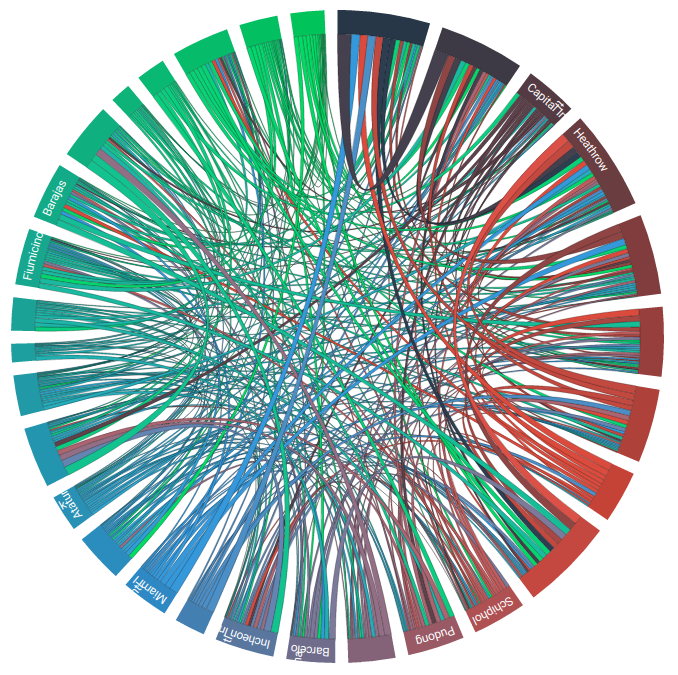
\includegraphics[width=100mm]{img/07_chord_highest_degree}
	\caption{D3.js Chord Visualizer: The air routes data set sampled with the \emph{highest degree} method. The algorithm apparently returns the 30 \emph{busiest} airports in the data set.}
    \label{fig:chord-highest-degree}
\end{figure}

\begin{figure}
	\centering
	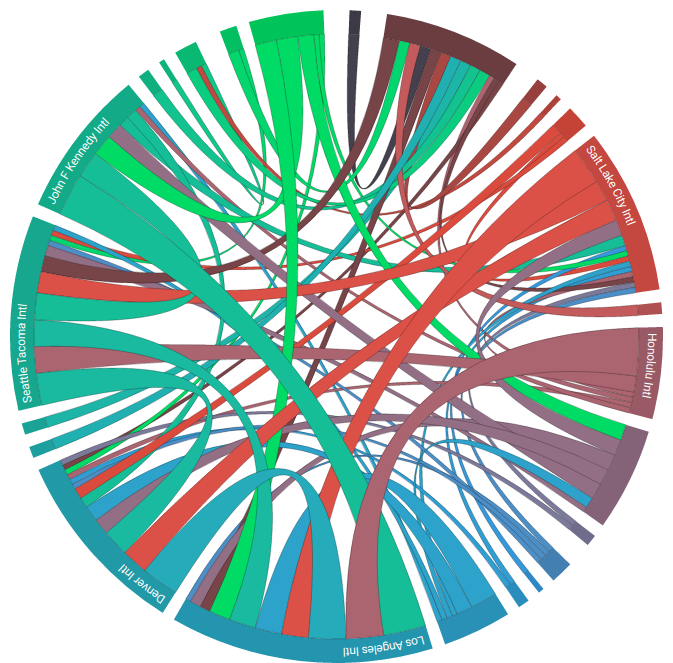
\includegraphics[width=100mm]{img/07_chord_forest_fire}
	\caption{D3.js Chord Visualizer: The air routes data set sampled with the Forest Fire method. The result is way more diverse as both small and big airports are displayed.}
    \label{fig:chord-forest-fire}
\end{figure}

We might say that whereas the \emph{highest degree} method is biased towards the most important nodes in the data set, the Forest Fire method will give the user a way more diverse result. Depending on a situation, both approaches might be useful. One of the possible improvements might be that we could let the user manually choose the sampling method as a way to explore the data set.

To sum it up, let us walk again through those three concerns we had regarding graph sampling.

\begin{itemize}
\item Compared to the \emph{highest degree} method, Forest Fire algorithm is less inclined to return independent sets which is thanks to the underlying BFS. Obviously, if most of the graph are independent nodes, then even Forest Fire algorithm could return an empty sample.
\item The complexity of Forest Fire algorithm does not depend on the graph size (except for the full graphs). That means that this algorithm will perform well even for very large graphs.
\item As of the \emph{resemblance} between the original graph and the sample, we explained that given the very small sample size, we cannot objectively measure this attribute. Nevertheless, Forest Fire algorithm does provide more diverse results.
\end{itemize}

Forest Fire algorithm clearly demonstrates its superiority and that is why we chose it as the default sampling algorithm.

There is one last remark we would like to make on this topic. The Forest Fire algorithm can be configured with the forward $p_f$ and backward $p_b$ probabilities. The forward probability is the probability of \emph{fire} \emph{spreading} over outgoing edges whereas the backward probability is the probability of \emph{fire} \emph{spreading} over incoming edges. In \cite{leskovec2006sampling} the authors try to determine the values for which they get the best results. As we already discussed, in our case it is hard to measure the resemblance between the original graph and the sample. We also mentioned that the authors of \cite{leskovec2006sampling} are a bit inconsistent in the exact algorithm description which makes it impossible to reproduce their results. Given this fact we slightly altered the algorithm: we used binomial distribution instead of geometric (as suggested in \cite{leskovec2005graphs}) because there is the nice BFS enhanced with \emph{coin flipping} analogy making the algorithm more straightforward to explain and implement. This all means that the values measured in \cite{leskovec2006sampling} are more or less irrelevant for us.

Nevertheless, this certainly does not mean that those parameters do not matter. With setting $p_f$ to $1$ (or a value close to $1$) we change the algorithm to standard BFS. So for example, if our first randomly selected node is a small American airport (from the air routes data set), the sample will contain only airports from that area. On the other hand, setting $p_f$ (and $p_b$) to $0$ turns off the search completely and we are simply selecting 30 random nodes from the data set. The sample is then completely arbitrary. We decided to leave $p_f$ to $0.2$ and $p_b$ to $0.05$ as suggested in  \cite{leskovec2006sampling}. These values produced \emph{reasonable} results and we had no reason to change them.

\todo[color=green!40]{Tady na konci jsem vynechal ten odstavec ohledně implementace (vytknul jste mi porušení SRP), asi není úplně potřeba}

\chapter{Future work}

There is lots of space for possible improvements of our \emph{application generator}. In this chapter, we will explore a couple of areas and explain what could be done better in those areas.

\section{Separating from LinkedPipies Visualization}

Our \emph{application generator} is integrated into the LinkedPipes Visualization. We justified this decision in Section \ref{sec:proposal:features} and as we suggested, this move did save us quite a lot of work. On the other hand, it led to certain schizophrenic situations. For example, whereas our \emph{application generator} contains a user layer (Subsection \ref{sec:implementation:overview:users}), LinkedPipes Visualization does not, but they do share the underlying instance of LDVM implementation. The consequence is that only an authenticated administrator is allowed to register a new \emph{visualizer} to our \emph{application generator} but literary anyone can use the LinkedPipes Visualization user interface to start uploading arbitrary LDVM components (an attacker could for example upload an extensive number of LDVM components which would slow down the \emph{discovery algorithm}, making it unusable).

Unfortunately, at this moment we cannot just turn off the LinkedPipes Visualization user interface as some of its functionality (specifically uploading new LDVM components, see Subsection \ref{sec:implementation:integrating-visualizer:ldvm}) is still required by our \emph{application generator}. Therefore, the first step would have be to implement the missing features to the \emph{application generator}, making it completely independent on LinkedPipes Visualization user interface.

Eventually, we need to come up with a strategy for separating these two tools. One way would be to make the \emph{application generator} the default user interface over the underlying LDVM implementation and definitely remove the current default one. This remains open. But as we explained in Section \ref{sec:implementation:general-architecture}, we made sure to keep the \emph{application generator} code as separated as possible which should simplify any potential future steps. 

\section{Platform features}

The \emph{platform} contains all the essential features but many of them are in a rather \emph{proof-of-concept} state.

\begin{itemize}
\item At this moment, it is only possible to choose application name and description. With some more information (rich text description, tags, theme category, screenshot) we could significantly improve the application catalog.
\item Similarly, each data source has only a name. It would be nice to be able to add some more information (such as description, category, author). In this case, this information could be automatically extracted from the data source itself (if it was available). Using this information, we could create a richer and more convenient data source browser. 
\item Another example is user authentication. At this moment, we support either Google users or local registration (which is not even verifying the e-mail provided by the user). Adding more account providers or improving the process of local registration would make sense.
\end{itemize}

In all these cases we just named, we typically needed a fast solution to prove that it works, and when we had it, we moved on to the next more pressing issue. In this matter, the platform could be improved and extended almost endlessly.

Nevertheless, there are couple of shortcomings that actually limit the way one can work with the \emph{application generator}. 

\begin{itemize}
\item At this moment, only data sources in the form of a SPARQL endpoint are accepted. It would be very helpful if the user could upload serialized RDF data directly or provide a HTTP link to such data.
\item The LDVM \emph{discovery} algorithm (Section \ref{sec:linkedpipes:ldvm-implementation}) offers to the user a list of discovered \emph{pipelines} to choose from. The problem is when there are several \emph{pipelines} ending with the same \emph{visualizer}. The user is given no leads on which he should select. Unfortunately, the only way to figure out what a \emph{pipeline} actually produces is to run it. But we could make this decision process somehow more convenient. Firstly, the \emph{pipeline} structure could be somehow visualized to the user. By examining the components in the \emph{pipeline} the user could get a better idea of what this \emph{pipeline} does. Secondly, we could somehow utilize the \emph{visualizer features}. Typically, a \emph{pipeline} ending with a \emph{visualizer} with more \emph{features} supported is a better \emph{pipeline}. Lastly, to examine the data produced by a \emph{pipeline}, the user always has to create a new application. It would be nice if the user could somehow get a preview of how a generated application from this data set would look like.
\item Currently, re-running a \emph{pipeline} is not supported, i.e., the application is always based on the data that were produced when the \emph{pipeline} was run for the first time. It would be useful to give the user the option to re-run a \emph{pipeline} or even schedule regular \emph{pipeline} executions. If the data sources were regularly updated, the application would reflect it. It would become \emph{live}.
\item There is one exception to the previous point and that is when a \emph{pipeline} contains only a \emph{visualizer} which is directly connected to the \emph{data source}. In such a case, the \emph{pipeline} does not do anything and the original \emph{data source} is considered to be the \emph{pipeline evaluation}. This makes the application \emph{live} as suggested in the previous paragraph. Unfortunately, that has disadvantages too. If the \emph{data source} gets corrupted or disappears (remember, it is a SPARQL endpoint which the user might not have under control), the application will stop working. Therefore it would be very useful, if the user could decide whether wants to be connected directly to the \emph{data source} or to make a local copy of the data.
\end{itemize}

\section{Framework}

One of the disadvantages of current solution regarding the frontend layer is that the whole user interface is bundled into a single file. There are advantages too (as explained in Section \ref{sec:implementation:frontend-architecture}), but the problem here is that the bundles are already fairly large and they will only grow in size as new \emph{visualizer} will get implemented. The Webpack bundler supports \emph{code splitting} which means that the whole bundle will be divided into smaller pieces that will be lazily fetched by the client side when required. That should decrease the loading times of the \emph{application generator}. Adding support for \emph{code splitting} might become a necessity once the bundle size gets past certain point.

We implemented two \emph{visualizers}: D3.js Chord Visualizer (Section \ref{sec:visualizers:chord}) and Google Maps Visualizer (Section \ref{sec:visualizers:google-maps}). They both provide a way to somehow \emph{reduce} the data set before visualizing. In the chord \emph{visualizer}, the user manually searches and selects graph nodes to be visualized. In the map \emph{visualizer}, it is possible to filter the data using categories. Both, the search and the filtering are tight to the individual \emph{visualizer}. But one could easily imagine that we would use filtering to select nodes for the chord visualization, and that we would use search to add points to the map visualization. Therefore it would make sense to separate the search and the filtering from the individual \emph{visualizers} and turn them into re-usable drop-in solutions that could be utilized when developing new \emph{visualizers}. One could easily imagine, that a \emph{visualizer} would support both of them and they would get automatically activated depending on the data characteristics (which could be expressed with LDVM component \emph{features}).

New \emph{visualizers} have to be implemented directly into the \emph{application generator} code base (Section \ref{sec:implementation:integrating-visualizer}). Thanks to the modern collaboration tools this does not present a real problem. The code base exists in a public Git repository and new \emph{visualizers} could get into the code base from \emph{forked} repositories \footnote{https://help.github.com/articles/fork-a-repo/} using \emph{pull requests} \footnote{https://help.github.com/articles/using-pull-requests/}. Nevertheless, our original intention was to make the individual \emph{visualizers} completely independent as separate projects. One would then \emph{install} new \emph{visualizers} to the \emph{application generator} from a public repository (we could utilize existing package repositories like Maven \footnote{http://search.maven.org/}). Unfortunately, we failed to deliver this feature due to a lack of time and there is a question whether the current architecture design would allow this kind of integration. But should this \emph{application generator} become a widely used tool, this feature would make a lot of sense.

\section{Visualizers}

Clearly, the more \emph{visualizers} our \emph{application generator} has, the more powerful it is. We implemented just two \emph{visualizers} to prove our concept but a large part of the future work should involve developing more new \emph{visualizers} (and in general more new LDVM components).

As explained in Section \ref{sec:system_proposal:integration}, all the \emph{visualizers} are very similar in their nature as they are very \emph{domain specific}. In that section, we mentioned that the original guidelines for this thesis suggest that the user should be able to combine together different views for different types of data. Such views should be possible to display in a selected predefined layout before publishing the app. We could actually implement a \emph{visualizer} that would support this kind of applications. Its LDVM \emph{descriptor} (Section \ref{sec:linkedpipes:ldvm-implementation}) would be very general, it would accept any kind of data. The actual analysis would be performed by the \emph{visualizer} itself and depending on the data, that it would find in the data set, it would offer to the user those simple widgets (or views) that the user could combine together and put them into the selected layout. Such a \emph{visualizer} would be probably very complicated and as it would be possible to leverage very little features of the \emph{application generator}, the question is whether it actually makes sense to implement it as a new \emph{visualizer}. Perhaps it should be rather a standalone application.

Nevertheless, there is an alternative approach. Both our \emph{visualizers} support embed mode. The D3.js Chord Visualizer makes even one extract step as it allows the user to publish each chord diagram separately. We could implement a \emph{meta-visualizer} that would allow the user to combine together applications generated by other real \emph{visualizers}. This \emph{meta-visualizer} would simply contain a grid of HTML \texttt{iframes} that would display the selected applications in embed mode. Clearly, the capabilities of such a \emph{meta-visualizer} would be fairly limited but one could achieve interesting results with it.

When describing the D3.js Chord Visualizer, we explained its limitation that it is not able to work with multiple graph instances within a single data source (Subsection \ref{sec:visualizers:chord:rgml}). The \emph{visualizer} simply expects all vertices and edges to belong to a single graph. To overcome this limitation, we would add support for multiple graph instances in a way that the individual instances would be detected by the \emph{visualizer} and the user could select which graph he intends to visualize. Unfortunately, the main reason behind this limitation is that because of the way the individual graph instances are represented in RDF, it is complicated to work with them (e.g. query vertices and edges belonging to a specific graph instance). Solving this problem would be the most challenging part.

We also briefly presented our simple solution for fulltext search through RDF data (Subsection \ref{sec:visualizers:chord:rgml}). The crucial disadvantage of our solution was that it was slow as each search required going through the whole data set (linear complexity). To get better performance, we would need to introduce some kind of indexing, either by relying on an external tool (as we briefly suggested in Subsection \ref{sec:visualizers:chord:rgml}) or by implementing our own. Perhaps the simplest solution would be to load the graph data into the H2 database (which is already available) and utilize its search engine. A more thorough analysis would be required.

\chapter*{Conclusion}
\addcontentsline{toc}{chapter}{Conclusion}

We implemented the proposed \emph{application generator} which enables users to generate interactive web applications from RDF data. The user starts by selecting a source of RDF data. The \emph{application generator} analyzes the data and offers a list of \emph{visualizers} that are able to visualize the data. The user selects the \emph{visualizer} he is interested in and uses it to generate a new application. The \emph{application generator} allows the user to configure the application and then publish it.

We examined several existing related tools which helped us to specify the list of features that we decided our \emph{application generator} should support. This also showed that compared to other data representation formats, Linked Data offer the biggest potential for automatic analysis and automatic application generation.

Our \emph{application generator} is integrated into LinkedPipes Visualization. It utilizes its underlying LDVM implementation for fully automated and easily extendable Linked Data analysis. We extended LinkedPipes Visualization with all the necessary functionality required by our \emph{application generator}. Specifically, we added support for two new RDF vocabularies, RGML and FRESNEL.

The biggest asset of \emph{application generator} is the \emph{configuration phase}. Each \emph{visualizer} provides a \emph{configurator} user interface unique to the type of data the \emph{visualizer} supports. The \emph{configurator} interface enables the user to configure the application before it gets published. The configuration possibilities differ depending on the \emph{visualizer}, but typically the user is allowed to filter the data and tune the level of the application interactivity for the audience. It is also possible for example to fix missing text labels for individual entities in the data set.

Our \emph{application generator} is \emph{non-developers friendly}. The whole process of generating a new application requires zero technical knowledge and anyone with the base computer skills is able to generate a new application.

Our \emph{application generator} works as a \emph{platform}. Every user has its own account which he uses to manage his published application. The \emph{application generator} contains a catalog of published applications and also a simple repository of available data source that any user can utilize to generate applications.

Our \emph{application generator} is a \emph{framework}. Firstly, the \emph{framework} defines a clear way how new \emph{visualizer} can be seamlessly integrated into the \emph{application generator} which makes it easily extendable. We explained the process of integration a new \emph{visualizer} in a step-by-step guide which is part of this thesis. Secondly, the \emph{framework} provides the developer with several read-to-use drop-in solutions for some common tasks that can significantly speed up the process of developing a new \emph{visualizer}. Those common tasks for example include saving and loading the application configuration or multiple language support.

To showcase the capabilities of the \emph{platform} and the \emph{framework}, we developed two \emph{visualizers}. The first one is D3.js Chord Visualizer which visualizes graph data represented in RDF with a chord diagram. While making this \emph{visualizer}, we implemented and analyzed algorithms for fulltext search, for calculating a graph adjacency matrix and for graph sampling, all of which over a graph represented in RDF. The second one is Google Maps visualizer which visualizes geospatial data on a map. This \emph{visualizer} already existed in LinkedPipes Visualization and we decided to re-implement it for our \emph{application generation} to show the benefits of the \emph{application generator} concept over LinkedPipes Visualization.

Clearly, our \emph{application generator} is only as powerful as its \emph{visualizers}. At the current state, there are only two very domain specific \emph{visualizers} which means that the generator will yield no results for most of the RDF data. It is important to note that unlike for example tabular data, the RDF data are very versatile in what kind of information they can carry. That makes it very hard (possibly impossible) to create an almighty universal \emph{visualizer} capable of visualizing any RDF data (unless the \emph{visualizer} is very simplistic). However, we are confident that given the way the \emph{application generator} is designed, being both a \emph{platform} and a \emph{framework}, it lays a solid ground for future potential extensions. We believe we fulfilled the goal of this thesis.



%%% Bibliography
%%% Bibliography (literature used as a source)
%%%
%%% We employ bibTeX to construct the bibliography. It processes
%%% citations in the text (e.g., the \cite{...} macro) and looks up
%%% relevant entries in the bibliography.bib file.
%%%
%%% The \bibliographystyle command selects, which style will be used
%%% for references from the text. The argument in curly brackets is
%%% the name of the corresponding style file (*.bst). Both styles
%%% mentioned in this template are included in LaTeX distributions.



\renewcommand{\bibname}{Bibliography}

%%% Generate the bibliography. Beware that if you cited no works,
%%% the empty list will be omitted completely.

\bibliography{bibliography}

%%% If case you prefer to write the bibliography manually (without bibTeX),
%%% you can use the following. Please follow the ISO 690 standard and
%%% citation conventions of your field of research.

% \begin{thebibliography}{99}
%
% \bibitem{lamport94}
%   {\sc Lamport,} Leslie.
%   \emph{\LaTeX: A Document Preparation System}.
%   2nd edition.
%   Massachusetts: Addison Wesley, 1994.
%   ISBN 0-201-52983-1.
%
% \end{thebibliography}


%%% Figures used in the thesis (consider if this is needed)
\listoffigures

%%% Tables used in the thesis (consider if this is needed)
%%% In mathematical theses, it could be better to move the list of tables to the beginning of the thesis.
\listoftables

%%% Abbreviations used in the thesis, if any, including their explanation
%%% In mathematical theses, it could be better to move the list of abbreviations to the beginning of the thesis.
\chapwithtoc{List of Abbreviations}
\begin{itemize}
\item \emph{CSV}: Comma-separated values
\item \emph{RDBMS}: Relational database management system
\item \emph{OSS}: Open-source software
\item \emph{GPS}: Global positioning system
\item \emph{YAML}: YAML Ain't Markup Language
\item \emph{DSL}: Domain-specific language
\item \emph{HTML}: HyperText Markup Language
\item \emph{CSS}: Cascading Style Sheets
\item \emph{TTL}: Terse RDF Triple Language
\item \emph{XML}: Extensible Markup Language
\item \emph{JSX}: JavaScript syntax extension
\end{itemize}

%%% Attachments to the master thesis, if any. Each attachment must be
%%% referred to at least once from the text of the thesis. Attachments
%%% are numbered.
%%%
%%% The printed version should preferably contain attachments, which can be
%%% read (additional tables and charts, supplementary text, examples of
%%% program output, etc.). The electronic version is more suited for attachments
%%% which will likely be used in an electronic form rather than read (program
%%% source code, data files, interactive charts, etc.). Electronic attachments
%%% should be uploaded to SIS and optionally also included in the thesis on a~CD/DVD.
\appendix
\chapter{Frontend development stack}
\label{att:devstack}

The following sections present a short extract from documentations of individual tools that were used for the \emph{application generator} frontend. Their purpose is not to substitute the documentation but merely to provide the reader with enough information so that he can understand our code.

\section{ES6 and Babel compiler}

The frontend is completely written using ECMAScript 2015 \cite{es6} (known as ES6) which is the 6th version of ECMAScript standard. JavaScript is an implementation of ECMAScript, available in all mainstream browsers. ES6 introduces many new language constructs which are, however, not all supported by the current JavaScript implementation. We use Babel \footnote{https://babeljs.io/} transpiler which converts our ES6 code into standard JavaScript.

We will mention some of the features that we frequently use.

\begin{verbatim}
// Arrow functions
[1, 2, 3].map(x => x * x);

// var is replaced with const (for constants) and let (for mutable variables)
const PI = 3.14;
let i = 1;
i++;

// Standard class syntax (the prototypical inheritance is still under the hood)
class Dog extends Animal {
  constructor(name) {
    super(name);
  }
}

// Enhanced Object Literals
const a = 2;
const b = 3;
const obj = { a, b };
obj.a === 2;
obj.b === 3;

// Desctructing
const obj = { a: 2, b: 3 };
const { a, b } = obj;
a === 2; // true
b === 3; // true

const arr = [1, 2, 3];
const [a, b] = obj;
a === 1; // true
b === 2; // true
\end{verbatim}

Perhaps the most important feature for us are ES6 modules. Each file is a module which \emph{imports} its dependencies and \emph{exports} values that make a public API of that module.

\begin{verbatim}
// lib/math.js

export const PI = 3.14;

export function add(a, b) {
  return a + b;
}

export const multiply = (a, b) => a * b;

export default { add, multiply, PI };
\end{verbatim}

There are several ways how a dependency can be \emph{imported}.

\begin{verbatim}
import { multiply, PI } from './lib/math'

const result = multiply(PI, 2);
\end{verbatim}

\begin{verbatim}
import * as math from './lib/math'

const result = math.add(math.PI, 2);
\end{verbatim}

\begin{verbatim}
import math from './lib/math'

const result = math.add(math.PI, 2);
\end{verbatim}

\section{npm}
npm \cite{npm} is a package manager for JavaScript. We use it to manage our JavaScript dependencies. They are all listed in the file \texttt{src/package.json}. Once installed, a package can be used with the standard \texttt{import} command.

\begin{verbatim}
import moment from 'moment'

 // prints current time and date, i.e. June 24th 2016, 8:52:00 pm
moment().format('MMMM Do YYYY, h:mm:ss a');
\end{verbatim}

Note that when importing a npm dependency, we do not use relative paths starting with a dot.

\section{React}
React \cite{react} is a JavaScript library for building user interfaces. The base building block is a React component.

\begin{verbatim}
import React from 'react'

const HelloMessage = ({ name }) => (
    <div>Hello <strong>{name}</strong></div>
  )

React.render(<HelloMessage name="Jon Snow" />, document.getElementById('container'));
\end{verbatim}


This is the simplest shortest example possible where a component works as a plain function. It takes some input data and prints user interface. The input data are in the form of \texttt{props} which are passed in the first argument (we use ES6 destructing to extract the name \texttt{prop}). The user interface is defined using a XML-like syntax called JSX. This component prints a greeting with the highlighted name. Using the last line, the component is mounted to a specific DOM node marked with an id equal to "container".

The components can be composed. 

\begin{verbatim}
const HelloMessage = ({ name }) => (
    <div>Hello <strong>{name}</strong></div>
  );
  
const MessageList = ({ names }) => (
    <ul>
      {names.map(name => 
        <li>
          <HelloMessage name={name} />
        </li>
      )}
    </ul>
  )

const names = ['Jon Snow', 'Tyrion'];
React.render(<MessageList names={names} />, document.getElementById('container'));
\end{verbatim}

This example will print a greeting for each name in the list. As you can see, we can easily combine HTML tags with our own components. The \texttt{props} are passed down to the components with the syntax that we use for specifying  standard HTML attributes.

The components can be interactive.

\begin{verbatim}
class Counter extends React.Component {
  constructor(props) {
    this.state = {
      value: props.initialValue
    }
  }
  
  increase() {
    this.setState({
      value: this.state.value + 1
    })
  }
  
  render() {
    const { value } = this.state;
    return (
      <input type="button" 
        onClick={() => this.increase()} 
        value={'Increase: ' + value} />
     );
  }
} 

React.render(<Counter initialValue={10} />, document.getElementById('container'));
\end{verbatim}

This component no longer works as a simple function as it maintains its own state. The state contains just a numeric value which is increased every time the user clicks the button. The value is displayed in the input label. Note that we cannot simply assign the new value to the \texttt{state} object, we need to use the \texttt{setState} method which is part of the React API.

In this case, the rendered UI is a function of the component \texttt{props} and the component \texttt{state}. Whereas the \texttt{props} are immutable (like function arguments), the \texttt{state} can be mutated within the component.

In React, \textbf{you do not mutate the user interface}. That means that you do not define how the user interface should transition between different states but instead, you specify how the interface should look like given the current \texttt{props} and \texttt{state}. Every time the \texttt{state} changes or new \texttt{props} are passed from the parent component, the whole UI is completely re-rendered. This significantly simplifies building interactive user interfaces. If nothing else, the number of possible component states is significantly lower than the number of possible transitions between those states.

The React API defines several life cycle methods.

\begin{verbatim}
class GreetOnMount extends React.Component {
  componentWillMount() {
   alert('This component is about to be mounted to the DOM tree!');
  }
  
  componentWillUnmount() {
   alert('This component is about to be unmounted from the DOM tree!');
  }
  
  render() {
   return <div />
  }
}
\end{verbatim}

We have used two life cycle methods, \texttt{componentWillMount} which is triggered when the component is about to appear, and \texttt{componentWillUnmount} which is triggered when the component is about to disappear from the screen. These methods are especially useful for components that fetch data from the server. The first method can be used to initiate the request and the second method to cancel the request or possibly do some cleanup.

\section{Redux}
\label{att:devstack:redux}

Using the MVC terminology, a React component would be called a \emph{controller-view}\footnote{\url{https://facebook.github.io/flux/docs/overview.html}}. It both handles the interaction with the user and the visual representation. In our code, we usually try to distinguish between controllers and views. We create either a component that is rather a controller, i.e., it handles user input but does not focus on the visuals, or a component that is rather a view, i.e., there is no business logic going on and the component focuses only on representing the data on the screen. By composing components of these two types we build the whole user interface.

The component state would correspond to the definition of the \emph{Model} layer. Nevertheless, this approach, i.e., storing everything in the state of React components, would not work for large-scale applications which would have a lot of state. The \emph{state} in this context can mean literary everything, starting all the data fetched from the server, ending with the list of open dialog windows. That is why we use Redux.

Redux \cite{redux} is, as explained by the authors, a "predictable state container for JavaScript apps"~\cite{redux} that evolved from the Flux ideas. Flux \cite{flux} is an application architecture that was designed specifically to work with React applications. Even though Redux is independent on React, they work extremely well together. 

Setting up Redux with React is a bit complicated so we skip it. It is not really necessary because it is already done for us in the fronted code base and we can immediately start using it. The more important thing is to understand how it works.

The core idea is that we move the state out of the components. Let us start with a simple example. Our \emph{state} will be just a single number. We want to be able to increment and decrement the number. For each such operation we create an \emph{action type}.

\begin{verbatim}
const INCREMENT = 'INCREMENT';
const DECREMENT = 'DECREMENT';
\end{verbatim}

It is good practice that we also define \emph{action creators}.

\begin{verbatim}
function increment() {
  return { type: INCREMENT };
}

function decrement() {
  return { type: DECREMENT };
}
\end{verbatim}

Now we define a special function called a \emph{reducer} which specifies how every \emph{action} transforms the \emph{state}.

\begin{verbatim}
function valueReducer(state = 0, action) {
  switch (action.type) {
    case INCREMENT:
      return state + 1
    case DECREMENT:
      return state - 1
    default:
      return state
  }
}
\end{verbatim}

The function takes the current \emph{state} and an \emph{action} as an argument. Depending on the \emph{action type} (and typically also \emph{action payload}), it transforms the \emph{state}. Important is that the function does not mutate the old \emph{state} but rather creates a completely new \emph{state} from the old \emph{state}. In this case the \emph{state} is just an integer which is by its nature immutable. If the \emph{state} was more complex, typically an object, we would need to make sure to create a new object  every time it changes.

From a \emph{reducer} we create a \emph{store} which represents a running instance of Redux. It holds the current \emph{state} and provides a \emph{dispatch} function that we use to apply the \emph{actions} on the \emph{state}. Note in the following code snippet, that invoking \texttt{increment()} does not increase the value. It simply returns an \emph{action} object which is then \emph{dispatched} and processed by the \emph{reducer}.

\begin{verbatim}
dispatch(increment());
dispatch(decrement());
\end{verbatim}

Now let us see how we bind this to a React component.

\begin{verbatim}
import React from 'react'
import { connect } from 'react-redux'

const Counter = ({ dispatch, value }) => (
  <div>
    {value}
    <input type="button" onClick={() => dispatch(increase())} label="Increase" />
    <input type="button" onClick={() => dispatch(decrease())} label="Decrease" />
  </div>
);

const mapStateToProps = state => ({
  value: state
});

export default connect(mapStateToProps)(Counter);
\end{verbatim}

This way we \emph{connected} the component to the \emph{store}. The \emph{dispatch} function is automatically injected to the component as a \emph{prop} which means that we can start \emph{dispatching} actions to modify the \emph{state}. The \emph{state} (in our case just a single integer) is also injected to the component through the \emph{props} but we have to specifically define how that should happen using the \texttt{mapStateToProps} function.

The process makes up a circle. The user clicks the button in the component and an \emph{action} is \emph{dispatched} to the \emph{reducer}. The \emph{reducer} updates the \emph{state} and the \emph{store} notifies the component of a change. The component re-renders with the updated value. As the \emph{state} can be changed only using \emph{actions}, the system behavior is predictable and very explicit. Redux offers a development mode in which it is very easy to monitor the \emph{actions} flowing through the system and how they change the \emph{state} (Figure \ref{fig:graph-visualizer}).

The \emph{reducers} can be composed and combined. Let us now add another reducer that will simply count the number of clicks.

\begin{verbatim}
function clickCountReducer(state = 0, action) {
  switch (action.type) {
    case INCREMENT:
    case DECREMENT:
      return state + 1
    default:
      return state
  }
}
\end{verbatim}

Now we combine the reducers together.

\begin{verbatim}
import { combineReducers } from 'redux'

const rootReducer = combineReducers({
  value: valueReducer,
  clickCount: clickCountReducer
});
\end{verbatim}

This creates a new \emph{reducer} that combines the other two \emph{reducers} together in a way that it maintains two values in an object where each value is updated by the corresponding \emph{reducer}. Whenever an \emph{action} is \emph{dispatched}, the root \emph{reducer} passes the \emph{action} to both child \emph{reducers}.

Suddenly, our \emph{state} is more complicated because it is an object with two values. We have to update the \texttt{mapStateToProps} function accordingly.

\begin{verbatim}
const Counter = ({ dispatch, value, clickCount }) => (
  // ...
);

const mapStateToProps = state => state;
\end{verbatim}

In this case, we could actually significantly simplify the function as the \emph{state} structure directly corresponds to the \emph{props} that we want to inject.

In a similar manner we could start adding more and more \emph{reducers} to fit the needs of the application (and the \emph{state} hierarchy would grow correspondingly). Our \emph{application generator} has only one single vast and deep \emph{state} that holds all the information. If we apply the React component hierarchy on this \emph{state} hierarchy (updated by the \emph{reducer} hierarchy), we get the user interface that is currently on the screen.  We can say that what you can see on the screen is a \emph{function} of the \emph{state}.

% TODO: show action creators using promises and thunks

\section{Reselect}

We use the \texttt{mapStateToProps} function to extract the values from the \emph{state} required by a component. That worked really well for our simple examples but  it would not scale with the increasing size and depth of the \emph{state} object.

The \emph{state} can be viewed as a database. It is a huge blob of data that any part of the application can access. It defines a clear API for making updates and the updates are always performed in transactions (that stems from the single-threaded nature of JavaScript but what also matters is that when an \emph{action} is \emph{dispatched}, it has to update all \emph{reducers} first before another \emph{action} can be \emph{dispatched}). What we miss is an API for selecting data from the database, i.e., the \emph{state}. We use Reselect \cite{reselect} for that.

We will re-use the last iteration of our example with the \texttt{valueReducer} and \texttt{clickCountReducer}.

\begin{verbatim}
import {  createStructuredSelector } from 'reselect'

// ... the component

const valueSelector = state => state.value;
const clickCountSelector = state => clickCount;

const selector = createStructuredSelector({
  value: valueSelector,
  clickCount: clickCountSelector
});

export default connect(selector)(Counter);
\end{verbatim}

A Reselect \emph{selector} is like a named database query. It extracts a specific piece of data from the \emph{state}. We defined two base \emph{selectors} that access directly the state and we combined them together. Our final \emph{selector} becomes the \texttt{mapStateToProps} function. What is important is that once a \emph{selector} is created, we do not have to care about how it is implemented. For us, it is just a query that returns the data we need. That separates us from the raw \emph{state} structure. Just like we have a \emph{reducer} hierarchy and a \emph{component} hierarchy, we can add a \emph{selector} hierarchy covering the whole \emph{state}.

Let us say that \texttt{state.auth.user.id} contains the ID of the currently authenticated user. We want to inject that ID into a component. This is the simple \texttt{mapStateToProps} approach:

\begin{verbatim}
const mapStateToProps = state => ({
  userId: state.auth.user.id
});
\end{verbatim}

With a smart \emph{selector} hierarchy, we could do this.

\begin{verbatim}
import { createSelector } from 'reselect'
import { userSelector } from './selectors'

const selector = createSelector(
  [userSelector],
  user => ({ userId: user.id }));
\end{verbatim}

Whereas in the first example, we actually have to know the complete \emph{state} hierarchy to extract this piece of information (and that can very often change due to refactoring), in the second example we are completely separated from the \emph{state} hierarchy and we just need to know the schema of the user object that the \texttt{userSelector} returns.

The selectors can do some extra calculations. Using a simple math formula we calculate the number of increment clicks. Clearly, we could maintain this information in another \emph{reducer} but as we can derive this information from information that is already in the state, it would be duplication.

\begin{verbatim}
const incrementCountSelector = createSelector(
  [valueSelector, clickCountSelector],
  (value, clickCount) => (clickCount + value) / 2);
\end{verbatim}

The \emph{selectors} can be arbitrarily combined.

\begin{verbatim}
const decrementCountSelector = createSelector(
  [clickCountSelector, incrementCountSelector],
  (clickCount, incrementCount) => clickCount - incrementCount);
\end{verbatim}

Every time the \emph{state} is updated, the \emph{selectors} are recalculated and consequently the \emph{components} are re-rendered. The \emph{selectors} are actually slightly smarter than that. The \emph{selector} output is automatically cached and if its input does not change, the cached value is returned instead. Therefore the \emph{selectors} can be used even for heavy computations.

\section{React-router}

As one would expect, our \emph{application generator} will consist of many different screens with different functionality. We need a mechanism for transitioning between those screens. Although many approaches are viable, we prefer the one with classic URLs, i.e., every different screen has its own URL. It has clear benefits as the user navigates through the interface as if it was a standard web page (e.g. even with the back button support).

Our \emph{application generator} is a SPA which means that each URL will contain the part corresponding to the actual physical address of the SPA (the entry URL) and the part maintained only by the frontend JavaScript application.

\begin{verbatim}
Sample URL: 
http://localhost:9000/appgen/dashboard/discoveries

SPA entry URL: 
http://localhost:9000/appgen/

Virtual URL part maintained by the SPA: 
dashboard/discoveries
\end{verbatim}

JavaScript API in modern web browsers allows us to change the URL without actually reloading the page.

We use React-router \cite{react-router} as a routing library for React. To show you how it works, we borrow an example from their documentation\footnote{\url{https://github.com/reactjs/react-router\#whats-it-look-like}}.

\begin{verbatim}
import React from 'react'
import { Route, IndexRoute } from 'react-router'

const App = ({ children }) => (
    <div>
      <h1>Welcome to our app</h1>
      {children}
    </div>
  );

const About = () => <h2>About</h2>

const Users = ({ children }) => (
    <div>
      <h2>Users</h2>
      {children}
    </div>
  );

const User = ({ params: { userId }}) => <div>User: <strong>{userId}</div>

const NoMatch = () => <h2>Not found</h2>

const routes = (
    <Route path="/" component={App}>
      <Route path="about" component={About}/>
      <Route path="users" component={Users}>
        <Route path=":userId" component={User}/>
      </Route>
      <Route path="*" component={NoMatch}/>
    </Route>
  );
\end{verbatim}

The React-router uses JSX for routes definition which makes it very declarative. For each route, we define a React component that is activated when the URL matches this particular route. The URL segment that has to be matched is defined by the \texttt{path} attribute, the component by the \texttt{component} attribute. The routes definition is hierarchical specifying the complete URL schema.

When a URL is matched, all components along the path of matching routes through the routes definition are activated. For example, for the URL \texttt{/users/15} the components \texttt{App}, \texttt{Users} and \texttt{User} are activated. The child component is always passed to the parent component through the \texttt{children prop}. 

As you might have noticed, all the tools in our stack introduce some kind of explicit composability. That is very useful because it will make all parts of our  \emph{application generator} easily extendable and re-usable.

\section{Immutable.js}

Immutable.js \cite{immutable} is a library containing  standard data structures that we may know for example from Java (e.g. \texttt{List}, \texttt{Map} or \texttt{Stack}). The core feature is that all the data structures are \emph{immutable} which means that they cannot be changed. If we change an instance of a \texttt{List} (e.g. by adding an element) we create a completely new instance and the old one remains unchanged. Consider the following example.

\begin{verbatim}
import { List } from 'immutable'

const list = new List();
const listUpdated = list.push(5);

list.size === 0;
listUpdated.size === 1;
\end{verbatim}

This library has many advantages. Firstly, it provides an extremely strong and well documented API which goes beyond the capabilities of standard JavaScript collections (\texttt{object} or \texttt{array}). The API fits better into the functional nature of our code. Secondly, it works really well with \emph{reducers}. As explained, a \emph{reducer} has to always return a new state which is sometimes a bit complicated using the standard JavaScript API. In the following example, we need to create a new copy of an object containing users identified by their IDs.

\begin{verbatim}
function usersReducer(state = {}, action) {
  switch (action.type) {
    case ADD_USER: 
      return Object.assign({}, state, {
        action.payload.id: action.payload.id
      })
    default:
      return state;
  }
}
\end{verbatim}

Now consider the version with Immutable.js.

\begin{verbatim}
import { Map } from 'immutable'

function usersReducer(state = new Map(), action) {
  switch (action.type) {
    case ADD_USER: 
      return state.set(action.payload.id, action.payload.id);
    default:
      return state;
  }
}
\end{verbatim}

Thirdly, there are some speed benefits as this is what makes the Reselect caching actually possible. A \emph{selector} recalculates only when the input arguments change. If an input argument was a standard mutable object, it would be very complicated (and expensive) to determine whether it changed. We would be keeping a reference to that object and have no idea whether the object was changed in the mean time. On the other hand, if we keep a reference to an immutable structure and the reference does not change, then we can be sure that the content of the referenced structure also did not change and we can re-use the cached value. Similar mechanism is used also for React components, i.e., it is possible to avoid unnecessary re-renders.

Lastly, Immutable.js library offers the \texttt{Record} data structure which is essentially a \texttt{Map} (i.e., a \emph{key-value} storage, just like a standard JavaScript \texttt{object}) but with an enforced schema.

\begin{verbatim}
const User = Record({
  id: 0,
  name: 'Anonymous user'
});

const user = new User({ id: 5, gender: 'male' });

user.id === 5;
user.name === 'Anonymous user';
user.gender === null;
\end{verbatim}

Any values that are missing during the instantiation are replaced with the default values and any values that are not part of the schema are removed. Unlike the standard immutable \texttt{Map}, a \texttt{Record} properties can be accessed using the standard dot notation (it even supports destructing). It is also very useful when we are defining the \texttt{propTypes} of a React component.

\begin{verbatim}
class UserView extends React.Component {
  static propTypes = {
    user: React.PropTypes.instanceOf(User).isRequired
  }
}
\end{verbatim}

If this component does not receive a \texttt{User} instance through the \texttt{props}, a warning is thrown.

\openright
\end{document}
